\documentclass[tocnosub,noragright,centerchapter,12pt,fullpage]{uiucecethesis09}


% Use draftthesis for notes and date markings on every page.  Useful when you
%   have multiple copies floating around.
% Use offcenter for the extra .5 inch on the left side. Needed with fullpage and fancy.
% Use mixcasechap for compatibility with hyperref package, which does NOT like all caps default
% Use edeposit for the adviser/committee on the title page.
% Use tocnosub to suppress subsection and lower entries in the TOC.
% PhD candidates use "proquest" for the proquest abstract.

\makeatletter

\usepackage{setspace}
%\usepackage{epsfig}  % for figures
\usepackage{graphicx}  % another package that works for figures
\usepackage{multirow}
\usepackage{placeins}
\usepackage{caption}  % allows center figures caption
\usepackage{booktabs} % nice rules (thick lines) for tables
\usepackage{array}
\usepackage{tabularx}
\newcolumntype{b}{>{\hsize=1.0\hsize}X}
\newcolumntype{s}{>{\hsize=.5\hsize}X}
\newcolumntype{m}{>{\hsize=.75\hsize}X}
\newcolumntype{x}{>{\hsize=.25\hsize}X}
\graphicspath{{figures/}}
%\usepackage{subfigure}  % for subfigures
\usepackage{amsmath}  % for math spacing
%\usepackage{amssymb}  % for math spacing
%\usepackage{url}  % Hyphenation of URLs.
\usepackage{lscape}  % Useful for wide tables or figures.
\usepackage[justification=raggedright]{caption}	% makes captions ragged right - thanks to Bryce Lobdell
\usepackage[acronym,toc]{glossaries}  % acronyms inclusion
\usepackage{color,soul}
\makeglossary

% Uncomment the appropriate one of the following four lines:
%\msthesis
%\phdthesis
%\otherdoctorate[abbrev]{Title of Degree}
%\othermasters[abbrev]{Title of Degree}

\title{Simulation tool for molten salt reactor neutronics and fuel cycle modeling with Serpent}
\author{Andrei Rykhlevskii}
\department{Nuclear, Plasma, and Radiological Engineering}
\degreeyear{2019}

% Advisor name is required for
% - doctoral students for the ProQuest abstract
% - master's students who do not have a master's committee
%\advisor{Professor Kathryn D. Huff}

% Uncomment the \committee command for
% - all doctoral students
% - master's students who have a master's committee
\committee{Kathryn Huff, Advisor\\
           Tomasz Kozlowski     \\
           James Stubbins    \\
           Luke Olson}   

\begin{document}
%\newacronym{<++>}{<++>}{<++>}
\newacronym[longplural={metric tons of heavy metal}]{MTHM}{MTHM}{metric ton of heavy metal}
\newacronym{ABM}{ABM}{agent-based modeling}
\newacronym{ACDIS}{ACDIS}{Program in Arms Control \& Domestic and International Security}
\newacronym{AHTR}{AHTR}{Advanced High Temperature Reactor}
\newacronym{ANDRA}{ANDRA}{Agence Nationale pour la gestion des D\'echets RAdioactifs, the French National Agency for Radioactive Waste Management}
\newacronym{ANL}{ANL}{Argonne National Laboratory}
\newacronym{ANS}{ANS}{American Nuclear Society}
\newacronym{AOA}{AOA}{Axial Offset Anomaly}
\newacronym{API}{API}{application programming interface}
\newacronym{ARE}{ARE}{Aircraft Reactor Experiment}
\newacronym{ARFC}{ARFC}{Advanced Reactors and Fuel Cycles}
\newacronym{ASME}{ASME}{American Society of Mechanical Engineers}
\newacronym{ATWS}{ATWS}{Anticipated Transient Without Scram}
\newacronym{BOL}{BOL}{Beginning of Life}
\newacronym{BDBE}{BDBE}{Beyond Design Basis Event}
\newacronym{BIDS}{BIDS}{Berkeley Institute for Data Science}
\newacronym{BWR}{BWR}{Boiling Water Reactor}
\newacronym{CAFCA}{CAFCA}{ Code for Advanced Fuel Cycles Assessment }
\newacronym{CDTN}{CDTN}{Centro de Desenvolvimento da Tecnologia Nuclear}
\newacronym{CFD}{CFD}{Computational Fluid Dynamics}
\newacronym{CEA}{CEA}{Commissariat \`a l'\'Energie Atomique et aux \'Energies Alternatives}
\newacronym{CI}{CI}{continuous integration}
\newacronym{CNEN}{CNEN}{Comiss\~{a}o Nacional de Energia Nuclear}
\newacronym{CNERG}{CNERG}{Computational Nuclear Engineering Research Group}
\newacronym{COSI}{COSI}{Commelini-Sicard}
\newacronym{COTS}{COTS}{commercial, off-the-shelf}
\newacronym{CSNF}{CSNF}{commercial spent nuclear fuel}
\newacronym{CTAH}{CTAHs}{Coiled Tube Air Heaters}
\newacronym{CUBIT}{CUBIT}{CUBIT Geometry and Mesh Generation Toolkit}
\newacronym{CURIE}{CURIE}{Centralized Used Fuel Resource for Information Exchange}
\newacronym{CR}{CR}{conversion ratio}
\newacronym{DAG}{DAG}{directed acyclic graph}
\newacronym{DANESS}{DANESS}{Dynamic Analysis of Nuclear Energy System Strategies}
\newacronym{DBE}{DBE}{Design Basis Event}
\newacronym{DESAE}{DESAE}{Dynamic Analysis of Nuclear Energy Systems Strategies}
\newacronym{DHS}{DHS}{Department of Homeland Security}
\newacronym{DOE}{DOE}{Department of Energy}
\newacronym{DRACS}{DRACS}{Direct Reactor Auxiliary Cooling System}
\newacronym{DRE}{DRE}{dynamic resource exchange}
\newacronym{DSNF}{DSNF}{DOE spent nuclear fuel}
\newacronym{DYMOND}{DYMOND}{Dynamic Model of Nuclear Development }
\newacronym{EBS}{EBS}{Engineered Barrier System}
\newacronym{EDF}{EDF}{Électricité de France}
\newacronym{EDZ}{EDZ}{Excavation Disturbed Zone}
\newacronym{EOL}{EOL}{End of Life}
\newacronym{EIA}{EIA}{U.S. Energy Information Administration}
\newacronym{EPA}{EPA}{Environmental Protection Agency}
\newacronym{EPR}{EPR}{European Pressurized Reactors}
\newacronym{EP}{EP}{Engineering Physics}
\newacronym{EU}{EU}{European Union}
\newacronym{FCO}{FCO}{Fuel Cycle Options}
\newacronym{FCT}{FCT}{Fuel Cycle Technology}
\newacronym{FEHM}{FEHM}{Finite Element Heat and Mass Transfer}
\newacronym{FEPs}{FEPs}{Features, Events, and Processes}
\newacronym{FHR}{FHR}{Fluoride-Salt-Cooled High-Temperature Reactor}
\newacronym{FLiBe}{FLiBe}{Fluoride-Lithium-Beryllium}
\newacronym{FP}{FP}{Fission Product}
\newacronym{GDSE}{GDSE}{Generic Disposal System Environment}
\newacronym{GDSM}{GDSM}{Generic Disposal System Model}
\newacronym{GENIUSv1}{GENIUSv1}{Global Evaluation of Nuclear Infrastructure Utilization Scenarios, Version 1}
\newacronym{GENIUSv2}{GENIUSv2}{Global Evaluation of Nuclear Infrastructure Utilization Scenarios, Version 2}
\newacronym{GENIUS}{GENIUS}{Global Evaluation of Nuclear Infrastructure Utilization Scenarios}
\newacronym{GPAM}{GPAM}{Generic Performance Assessment Model}
\newacronym{GRSAC}{GRSAC}{Graphite Reactor Severe Accident Code}
\newacronym{GUI}{GUI}{graphical user interface}
\newacronym{HFP}{HFP}{hot full power}
\newacronym{HLW}{HLW}{high level waste}
\newacronym{HPC}{HPC}{high-performance computing}
\newacronym{HTC}{HTC}{high-throughput computing}
\newacronym{HTGR}{HTGR}{High Temperature Gas-Cooled Reactor}
\newacronym{HZP}{HZP}{hot zero power}
\newacronym{IAEA}{IAEA}{International Atomic Energy Agency}
\newacronym{IEMA}{IEMA}{Illinois Emergency Mangament Agency}
\newacronym{IHLRWM}{IHLRWM}{International High Level Radioactive Waste Management}
\newacronym{INL}{INL}{Idaho National Laboratory}
\newacronym{IPRR1}{IRP-R1}{Instituto de Pesquisas Radioativas Reator 1}
\newacronym{IRP}{IRP}{Integrated Research Project}
\newacronym{ISFSI}{ISFSI}{Independent Spent Fuel Storage Installation}
\newacronym{ISRG}{ISRG}{Independent Student Research Group}
\newacronym{JFNK}{JFNK}{Jacobian-Free Newton Krylov}
\newacronym{LANL}{LANL}{Los Alamos National Laboratory}
\newacronym{LBNL}{LBNL}{Lawrence Berkeley National Laboratory}
\newacronym{LCOE}{LCOE}{levelized cost of electricity}
\newacronym{LEU}{LEU}{low-enriched uranium}
\newacronym{LDRD}{LDRD}{laboratory directed research and development}
\newacronym{LFR}{LFR}{Lead-Cooled Fast Reactor}
\newacronym{LLNL}{LLNL}{Lawrence Livermore National Laboratory}
\newacronym{LMFBR}{LMFBR}{Liquid Metal Fast Breeder Reactor}
\newacronym{LOFC}{LOFC}{Loss of Forced Cooling}
\newacronym{LOHS}{LOHS}{Loss of Heat Sink}
\newacronym{LOLA}{LOLA}{Loss of Large Area}
\newacronym{LP}{LP}{linear program}
\newacronym{LWR}{LWR}{Light Water Reactor}
\newacronym{MAGNOX}{MAGNOX}{Magnesium Alloy Graphie Moderated Gas Cooled Uranium Oxide Reactor}
\newacronym{MA}{MA}{minor actinide}
\newacronym{MCNP}{MCNP}{Monte Carlo N-Particle code}
\newacronym{MILP}{MILP}{mixed-integer linear program}
\newacronym{MIT}{MIT}{the Massachusetts Institute of Technology}
\newacronym{MOAB}{MOAB}{Mesh-Oriented datABase}
\newacronym{MOOSE}{MOOSE}{Multiphysics Object-Oriented Simulation Environment}
\newacronym{MOSART}{MOSART}{Molten Salt Actinide Recycler and Transmuter}
\newacronym{MOX}{MOX}{mixed oxide}
\newacronym{MPI}{MPI}{Message Passing Interface}
\newacronym{MSBR}{MSBR}{Molten Salt Breeder Reactor}
\newacronym{MSFR}{MSFR}{Molten Salt Fast Reactor}
\newacronym{MSRE}{MSRE}{Molten Salt Reactor Experiment}
\newacronym{MSR}{MSR}{Molten Salt Reactor}
\newacronym{NAGRA}{NAGRA}{National Cooperative for the Disposal of Radioactive Waste}
\newacronym{NEAMS}{NEAMS}{Nuclear Engineering Advanced Modeling and Simulation}
\newacronym{NEUP}{NEUP}{Nuclear Energy University Programs}
\newacronym{NFCSim}{NFCSim}{Nuclear Fuel Cycle Simulator}
\newacronym{NGNP}{NGNP}{Next Generation Nuclear Plant}
\newacronym{NMWPC}{NMWPC}{Nuclear MW Per Capita}
\newacronym{NNSA}{NNSA}{National Nuclear Security Administration}
\newacronym{NPP}{NPP}{Nuclear Power Plant}
\newacronym{NPRE}{NPRE}{Department of Nuclear, Plasma, and Radiological Engineering}
\newacronym{NQA1}{NQA-1}{Nuclear Quality Assurance - 1}
\newacronym{NRC}{NRC}{Nuclear Regulatory Commission}
\newacronym{NSF}{NSF}{National Science Foundation}
\newacronym{NSSC}{NSSC}{Nuclear Science and Security Consortium}
\newacronym{NUWASTE}{NUWASTE}{Nuclear Waste Assessment System for Technical Evaluation}
\newacronym{NWF}{NWF}{Nuclear Waste Fund}
\newacronym{NWTRB}{NWTRB}{Nuclear Waste Technical Review Board}
\newacronym{OCRWM}{OCRWM}{Office of Civilian Radioactive Waste Management}
\newacronym{OOP}{OOP}{Object-Orienting Programming}
\newacronym{ORION}{ORION}{ORION}
\newacronym{ORNL}{ORNL}{Oak Ridge National Laboratory}
\newacronym{PARCS}{PARCS}{Purdue Advanced Reactor Core Simulator}
\newacronym{PBAHTR}{PB-AHTR}{Pebble Bed Advanced High Temperature Reactor}
\newacronym{PBFHR}{PB-FHR}{Pebble-Bed Fluoride-Salt-Cooled High-Temperature Reactor}
\newacronym{PEI}{PEI}{Peak Environmental Impact}
\newacronym{PH}{PRONGHORN}{PRONGHORN}
\newacronym{PRIS}{PRIS}{Power Reactor Information System}
\newacronym{PRKE}{PRKE}{Point Reactor Kinetics Equations}
\newacronym{PSPG}{PSPG}{Pressure-Stabilizing/Petrov-Galerkin}
\newacronym{PWAR}{PWAR}{Pratt and Whitney Aircraft Reactor}
\newacronym{PWR}{PWR}{Pressurized Water Reactor}
\newacronym{PyNE}{PyNE}{Python toolkit for Nuclear Engineering}
\newacronym{PyRK}{PyRK}{Python for Reactor Kinetics}
\newacronym{QA}{QA}{quality assurance}
\newacronym{RDD}{RD\&D}{Research Development and Demonstration}
\newacronym{RD}{R\&D}{Research and Development}
\newacronym{REE}{REE}{rare earth element}
\newacronym{RELAP}{RELAP}{Reactor Excursion and Leak Analysis Program}
\newacronym{RIA}{RIA}{Reactivity Insertion Accident}
\newacronym{RIF}{RIF}{Region-Institution-Facility}
\newacronym{SFR}{SFR}{Sodium-Cooled Fast Reactor}
\newacronym{SINDAG}{SINDA{\textbackslash}G}{Systems Improved Numerical Differencing Analyzer $\backslash$ Gaski}
\newacronym{SKB}{SKB}{Svensk K\"{a}rnbr\"{a}nslehantering AB}
\newacronym{SNF}{SNF}{spent nuclear fuel}
\newacronym{SNL}{SNL}{Sandia National Laboratory}
\newacronym{STC}{STC}{specific temperature change}
\newacronym{SUPG}{SUPG}{Streamline-Upwind/Petrov-Galerkin}
\newacronym{SVF}{SVF}{salt volume fraction}
\newacronym{SWF}{SWF}{Separations and Waste Forms}
\newacronym{SWU}{SWU}{Separative Work Unit}
\newacronym{TAP}{TAP}{Transatomic Power}
\newacronym{TRIGA}{TRIGA}{Training Research Isotope General Atomic}
\newacronym{TRISO}{TRISO}{Tristructural Isotropic}
\newacronym{TSM}{TSM}{Total System Model}
\newacronym{TSPA}{TSPA}{Total System Performance Assessment for the Yucca Mountain License Application}
\newacronym{ThOX}{ThOX}{thorium oxide}
\newacronym{UFD}{UFD}{Used Fuel Disposition}
\newacronym{UML}{UML}{Unified Modeling Language}
\newacronym{UOX}{UOX}{uranium oxide}
\newacronym{UQ}{UQ}{uncertainty quantification}
\newacronym{US}{US}{United States}
\newacronym{UW}{UW}{University of Wisconsin}
\newacronym{VISION}{VISION}{the Verifiable Fuel Cycle Simulation Model}
\newacronym{VVER}{VVER}{Voda-Vodyanoi Energetichesky Reaktor (Russian Pressurized Water Reactor)}
\newacronym{VV}{V\&V}{verification and validation}
\newacronym{WIPP}{WIPP}{Waste Isolation Pilot Plant}
\newacronym{YMR}{YMR}{Yucca Mountain Repository Site}

%%%%%%%%%%%%%%%%%%%%%%%%%%%%%%%%%%%%%%%%%%%%%%%%%%%%%%%%%%%%%%%%%%%%%%%%%%%%%%%
% TITLE
%
\maketitle

%\raggedright
\parindent 1em%

\frontmatter

%%%%%%%%%%%%%%%%%%%%%%%%%%%%%%%%%%%%%%%%%%%%%%%%%%%%%%%%%%%%%%%%%%%%%%%%%%%%%%%
% ABSTRACT
%
%\begin{abstract}
% Put the abstract in a file called "abs.tex" and it'll be inputted here.
%In the search for new ways to generate carbon-free, reliable 
base-load power, interest in advanced nuclear energy technologies, 
particularly \glspl{MSR}, has resurged with multiple new companies 
pursuing \gls{MSR} commercialization. To further develop these \gls{MSR} 
concepts, researchers need simulation tools for analyzing liquid-fueled 
\gls{MSR} depletion and fuel processing. However, current nuclear reactor 
physics software is unable to perform a depletion calculations for a 
reactor systems with online separations and feeds. This work proposes to 
develop a Python package, SaltProc, which couples 
with the Monte Carlo code, SERPENT2 to realistically simulate a generic 
\gls{MSR} online reprocessing system by modeling the changing isotopic 
composition of \gls{MSR} fuel salt. The SaltProc package will enable 
the simulation of neutron poisons extraction based on physics- and 
chemistry-driven correlations rather than assuming ideal 
removal efficiency. A few perspective liquid-fueled 
\gls{MSR} concepts among various fuel cycles, number of salts
(single- and two-fluid), neutron spectra and reprocessing schemes 
will be investigated to demonstrate and validate proposed simulation 
package.
%\end{abstract}

%%%%%%%%%%%%%%%%%%%%%%%%%%%%%%%%%%%%%%%%%%%%%%%%%%%%%%%%%%%%%%%%%%%%%%%%%%%%%%%
% DEDICATION
%
%\begin{dedication}
%Dedicated to the memory of my father, Igor Rykhlevskii, who always believed in my ability to %succeed in the academic arena.
%\end{dedication}

%%%%%%%%%%%%%%%%%%%%%%%%%%%%%%%%%%%%%%%%%%%%%%%%%%%%%%%%%%%%%%%%%%%%%%%%%%%%%%%
% ACKNOWLEDGMENTS
%
% Put acknowledgments in a file called "ack.tex" and it'll be inputted here.
%\begin{acknowledgments}
%\input{ack}
%\end{acknowledgments}																																				
%%%%%%%%%%%%%%%%%%%%%%%%%%%%%%%%%%%%%%%%%%%%%%%%%%%%%%%%%%%%%%%%%%%%%%%%%%%%%%%
% TABLE OF CONTENTS
%
\tableofcontents

%%%%%%%%%%%%%%%%%%%%%%%%%%%%%%%%%%%%%%%%%%%%%%%%%%%%%%%%%%%%%%%%%%%%%%%%%%%%%%%
% LIST OF TABLES
%
% The List of Tables is not strictly necessary. Omitting the List of Tables will
% simplify the thesis check and reduce the number of corrections.
%\listoftables

%%%%%%%%%%%%%%%%%%%%%%%%%%%%%%%%%%%%%%%%%%%%%%%%%%%%%%%%%%%%%%%%%%%%%%%%%%%%%%%
% LIST OF FIGURES
%
% The List of Figures is not strictly necessary. Omitting the List of Figures will
% simplify the thesis check and reduce the number of corrections.
%\listoffigures

%%%%%%%%%%%%%%%%%%%%%%%%%%%%%%%%%%%%%%%%%%%%%%%%%%%%%%%%%%%%%%%%%%%%%%%%%%%%%%%
% LIST OF ABBREVIATIONS
%
% The List of Abbreviations is not strictly necessary.
%\chapter{LIST OF ABBREVIATIONS}

%\printacronyms
%\begin{symbollist*}
%\item[MSBR] Molten Salt Breeder Reactor
%\item[MSR] Molten Salt Reactor
%\item[ORNL] Oak Ridge National Laboratory
%\end{symbollist*}


%%%%%%%%%%%%%%%%%%%%%%%%%%%%%%%%%%%%%%%%%%%%%%%%%%%%%%%%%%%%%%%%%%%%%%%%%%%%%%%
% LIST OF SYMBOLS
%
%\begin{symbollist}[0.7in]
%\item[$\tau$] Time taken to drink one cup of coffee.
%\end{symbollist}

\mainmatter

%%%%%%%%%%%%%%%%%%%%%%%%%%%%%%%%%%%%%%%%%%%%%%%%%%%%%%%%%%%%%%%%%%%%%%%%%%%%%%%
% INSERT REAL CONTENT HERE
%
\chapter[Introduction]{Introduction}
\section{Motivation}
Humankind has only a few ways to generate reliable, nonintermittent baseload 
power: fossil fuels, hydro-power, geothermal power, and nuclear energy. 
Because of increasing global climate change concerns, sources with negligible 
CO$_2$ footprints are crucial measures for global temperature control. Thus, 
from an environmental viewpoint, hydro and nuclear power are preferable ways 
to generate reliable power. Nevertheless, the potential for a hydro-power is 
strictly limited by local geographical conditions; hence, the only option left 
is nuclear power. Nuclear power plants provided 10\% of global electricity 
supply in 2018 \cite{iea_nuclear_2019}. Moreover, nuclear share in energy 
generation is projected to stay constant through 2040, while electricity 
demand will increase by 30\% \cite{noauthor_world_2017}. 

The Generation IV International Forum (GIF) chose \glspl{MSR} among the six 
advanced reactor concepts for further research and development. \glspl{MSR} 
offer significant improvements ``in the four broad areas of sustainability, 
economics, safety and reliability, and proliferation resistance and physical 
protection" \cite{doe_technology_2002}. To achieve the goals formulated by the 
GIF, \glspl{MSR} simplify the reactor core and improve inherent safety by 
using liquid coolant which is also a fuel\footnote{Herein \glspl{MSR} are 
assumed to be reactors with liquid fuel which simultaneously serves 
as coolant.}. In a thermal spectrum \gls{MSR}, liquid fuel consists 
of carrier salt (i.e. LiF, LiF-BeF$_2$ or LiF-NaF-KF) and fluorides of fissile 
and/or fertile materials (i.e. UF$_4$, PuF$_3$ and/or ThF$_4$). This fuel  
circulates in a loop-type primary circuit \cite{haubenreich_experience_1970}. 
This innovation leads to immediate advantages over traditional, 
solid-fueled, reactors. These include near-atmospheric pressure 
in the primary loop, relatively high coolant temperature, outstanding 
neutron economy, a high level of inherent safety, reduced fuel 
preprocessing, the ability to continuously remove fission products 
and add fissile and/or fertile elements without shutdown 
\cite{leblanc_molten_2010}. The possibility of continuously removing 
neutron poisons increases the potential fuel burnup and thus 
improves the resource utilization of \glspl{MSR}. Finally, the \gls{MSR} 
also could be employed for transmutation of 
spent fuel from current \glspl{LWR} \cite{fratoni_design_2004}.

Recently, interest in \glspl{MSR} has resurged, with multiple new companies 
pursuing commercialization of \gls{MSR} designs\footnote{Examples 
include liquid-fueled \gls{MSR} designs from Terrapower, Terrestrial, 
ThorCon, Flibe, Copenhagen Atomics, Elysium, etc.}. China's \gls{MSR} program 
was initiated in 2011 and promises to startup a 2MW$_{th}$ 
liquid-fueled test \gls{MSR} in 2020, a 10MW$_{th}$ 
demonstration reactor in 2025, and a gigawatt-level 
commercial reactor in 2050 \cite{zhang_review_2018}. The European 
Union funds the Safety Assessment of the Molten Salt Fast Reactor 
(SAMOFAR) project, in which several European research institutes and 
universities are developing various molten salt reactor prototypes 
such as the \gls{MSFR} \cite{fiorina_molten_2013} and the \gls{MOSART} 
\cite{ignatiev_molten_2014}. To advance these \gls{MSR} concepts, particularly 
concerning their strategies for online reprocessing and refueling, 
we need computational analysis methods capturing their unique reactor physics, 
fuel reprocessing mechanics, and chemistry. 

The main objective of the proposed work is to develop the online 
reprocessing simulation package, SaltProc, which couples with the 
continuous-energy Monte Carlo depletion calculation code, Serpent 2 
\cite{leppanen_serpent_2014}, for liquid-fueled \gls{MSR} depletion 
simulations. Most of existing \gls{MSR} depletion simulators usually assume 100\% 
efficiency of the neutron poison removal process (see Chapter 1). The ultimate 
objective of this effort is to develop a generic open-source tool capable of 
simulating a wide range of liquid-fueled systems --- including two-fluid and
multi-region designs --- and to validate it against existing modeling efforts. 
Moreover, SaltProc enables poison extraction simulation based on a 
realistic physics-based fuel processing model.

This document outlines the motivation, preliminary work, and future work 
proposed towards developing a simulation tool for analyzing fuel depletion in 
a liquid-fueled \glspl{MSR}. Chapter 1 serves as a literature review, 
providing background on fuel burnup, online fuel reprocessing approaches, 
safety parameter evolution during reactor operation, and how these 
concepts have been applied to a wide range of \glspl{MSR} in the literature. 
Chapter 2 covers modeling online reprocessing details and proposed computation 
tool architecture. Chapter 3 explains the \gls{VV} method, demonstration 
cases, and safety parameter evolution. Specifically, these demonstration and 
verification efforts will focus on the \gls{TAP} \gls{MSR} because it is well 
analyzed in the literature. Chapter 4 gives the safety parameter overview and 
outlines the plan for analyzing these parameters' evolution during \gls{TAP} 
reactor lifetime. Finally, remaining future work and expected contributions to 
the nuclear community are summarized in Chapter 5.

\section{Fuel burnup and online reprocessing}
All liquid-fueled \gls{MSR} designs involve varying levels of online fuel 
processing. Minimally, volatile gaseous fission products (e.g., Kr, Xe) 
escape from the fuel salt during routine reactor operation and must be 
captured. Additional systems might be used to enhance the removal of those 
elements. Most designs also call for the removal of rare earth metals from 
the core since these metals act as neutron poisons. Some designs suggest a 
more elaborate list of elements to process (figure~\ref{fig:periodic_tab}), 
including the temporary removal of protactinium from the salt or other 
regulation of the actinide inventory in the fuel salt 
\cite{ahmad_neutronics_2015}. Fresh fuel salt with dissolved fissile and/or 
fertile material (e.g., $^{233}$U, $^{232}$Th, \gls{LEU}, a transuranic 
vector from \gls{LWR} \gls{SNF}) make up the salt mass loss caused by poison 
removal and conserves the total mass in the primary loop.
\begin{figure}[htp!] % replace 't' with 'b' to 
  \centering
  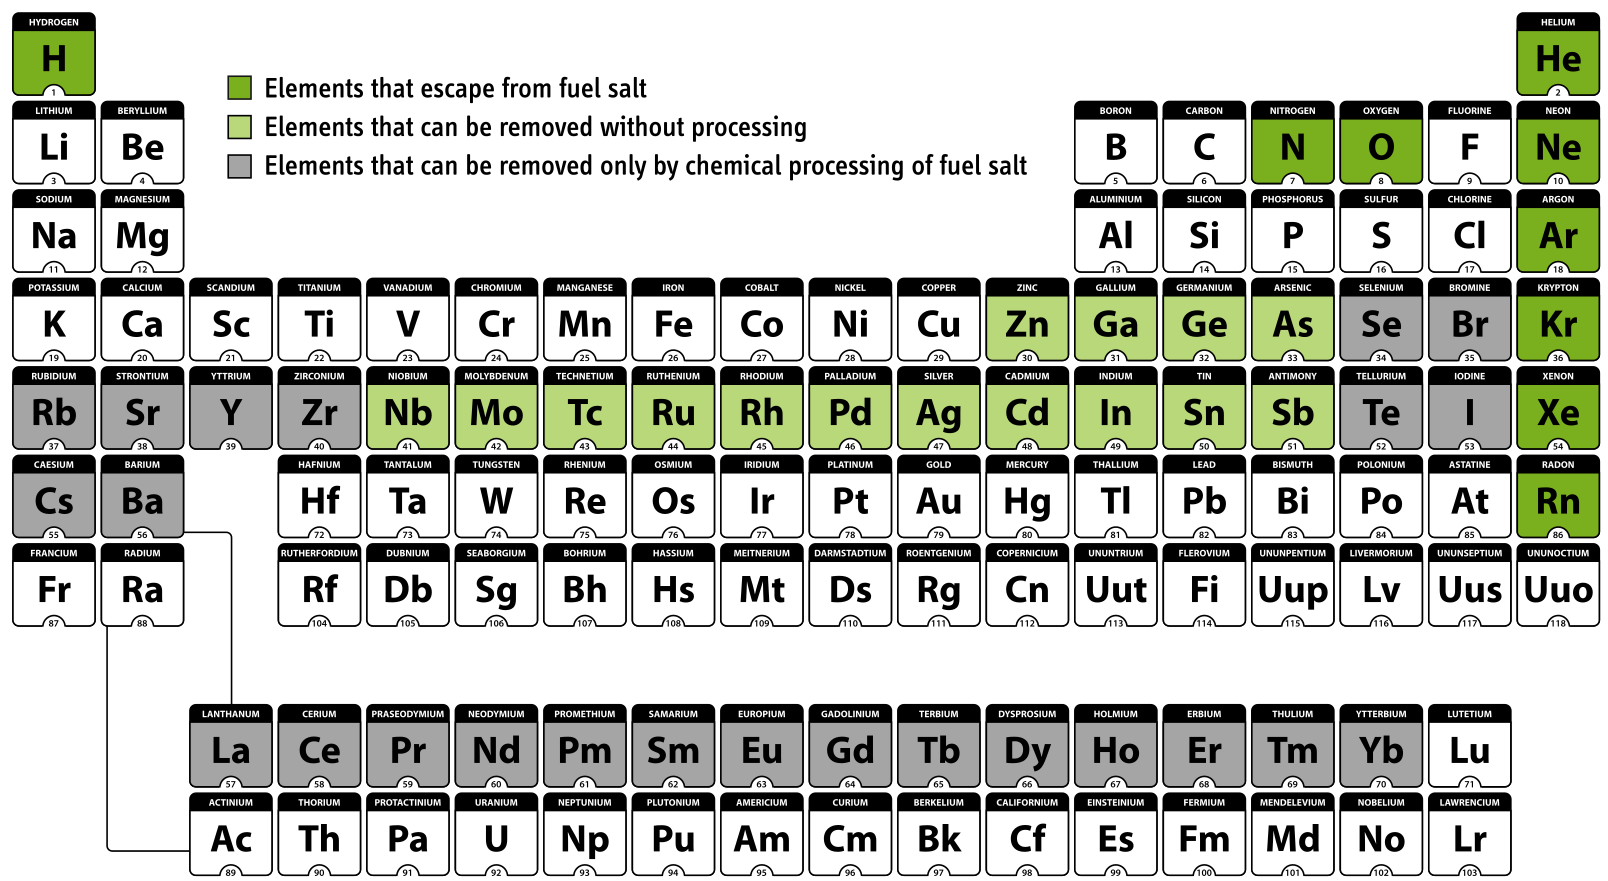
\includegraphics[width=0.9\textwidth]{periodic_map.png}
  \caption{Processing options for \gls{MSR} fuels (figure reproduced from 
  Ahmed \emph{et al.} \cite{ahmad_neutronics_2015}).}
  \label{fig:periodic_tab}
\end{figure}

Most liquid-fueled nuclear reactor concepts adopt nonintermittent separations 
and feeds: the core material is circulated to or from the core at all times 
(continuously) or specific intervals (batch-wise). In contrast, in a 
solid-fueled reactor, fission products and actinides remain within the initial 
fuel material during and after the operation until reprocessing. The ability 
to perform online fuel salt reprocessing improves the potential neutronics 
performance of liquid-fueled reactors. First, liquid-fueled reactors can 
operate with a relatively small excess reactivity because fissile material is 
continuously being added to the core. Second, continuously 
removing fission products, including strong absorbers (poisons) should 
significantly improve fuel utilization and decrease parasitic neutron 
absorption. Finally, for a breeder\footnote{\gls{CR} 
$\equiv$ fissile generated/fissile consumed: if CR $<$ 1, the reactor is a 
``converter''; CR $\equiv$ 1, an ``isobreeder''; CR $>$ 1, a 
``breeder.''} excess of fissile material might be continuously extracted  
from the core and used to start up new reactors. Nevertheless, the removal of 
each element from the liquid fuel salt presents a unique challenge in terms of 
chemical separation, storage, and disposal of the separated materials.

Continuous fuel salt reprocessing prevents the usage of most contemporary 
nuclear reactor fuel burnup software. To handle the material flows and 
potential online removal and feed of liquid-fueled systems, early \gls{MSR} 
simulation methods at \gls{ORNL}, which integrated neutronic and fuel cycle 
codes (i.e., Reactor Optimum Design (ROD) \cite{bauman_rod_1971}) into 
operational plant tools (i.e., Multiregion Processing Plant (MRPP) 
\cite{kee_mrpp_1976}) for \gls{MSR} fuel reprocessing system design. A summary 
of recent efforts is listed in table~\ref{tab:msr_codes}.
\begin{table}[t]
\fontsize{9}{11}\selectfont
\caption{Tools and methods for liquid-fueled \glspl{MSR} fuel salt depletion 
analysis.}
\begin{tabularx}{\textwidth}{X X X X X} 
\hline 
&Nuttin \emph{et al.}, 2005 \cite{nuttin_potential_2005}& Aufiero \emph{et al.}, 
2013 \cite{aufiero_extended_2013} & Betzler \emph{et al.}, 2018 
\cite{betzler_fuel_2018}&Proposed work \\ [12pt]
\hline
Neutron transport software & \gls{MCNP} & Serpent 2 & SCALE6.2 & Serpent 2 \\ 
[12pt]
Neutron transport method & \multicolumn{2}{c}{Monte Carlo continuous energy} & 
Deterministic discrete ordinates & Monte Carlo continuous energy \\ [12pt]
Burnup software & REM & Serpent 2 & ORIGEN-S & Serpent 2 \\ 
[12pt]
Geometry model & unit cell & full-core 3D & unit cell & full-core 3D\\ [12pt]
\gls{FP} removal/feed  & continuous &continuous & batch-wise & batch-wise\\ 
[12pt]
Separation efficiency &\multicolumn{3}{c}{fixed, must be defined by user 
before simulation} & variable of many parameters \\ [12pt]
Fuel reprocessing plant & \multicolumn{3}{c}{single component, ``black'' box 
model} & realistic multi-component model \\ [12pt]
Reactivity control & \multicolumn{2}{c}{continuous adjustment of fissile 
material injection} & batch injection of fissile material & periodical 
adjustment of geometry and fissile material injection\\
\hline
\end{tabularx}
  \label{tab:msr_codes}
\end{table}

Two main online reprocessing simulation approaches are commonly used in the 
literature: continuous and batch-wise. In the batch-wise approach, the burnup 
simulation stops at a given time and restarts with a new liquid fuel 
composition (after removal of discarded materials and addition of 
fissile/fertile materials). 

Accounting for continuous removal or addition of material presents a greater 
challenge since it requires adding a term to the Bateman equations. In 
SCALE/TRITON, ORIGEN \cite{gauld_isotopic_2011} solves a set of the Bateman 
equations using one-group averaged fluxes and cross sections obtained from a 
transport calculation. The Bateman equations describe the rate of change of 
each isotope, $i$, due to neutron induced reactions and decay processes
\cite{tsoulfanidis_nuclear_2013}:
\begin{align} \label{eq:bateman}
\frac{dN_i}{dt} &= \sum_{m=1}^{M}l_{im}\lambda_mN_m + 
\phi\sum_{m=1}^{M}f_{im}\sigma_mN_m - (\lambda_i + \phi\sigma_i + r_i - 
f_i)N_i + F_i\Big|{i\in [1,M]}\\
& \qquad\qquad (1) \qquad\qquad\qquad (2) \qquad\qquad(3) \quad (4)  \quad 
(5) \quad (6)
\nonumber
\intertext{where}
N_i &= \mbox{atom density of nuclide i} \nonumber \\
M &= \mbox{number of nuclides} \nonumber \\
l_{im} &= \mbox{fraction of decays of nuclide m that result in formation of 
nuclide i}\nonumber \\
\lambda_i &= \mbox{radioactive decay constant of nuclide i} \nonumber \\
\phi &= \mbox{neutron flux, averaged over position and energy} \nonumber \\
f_{im} &= \mbox{fraction of neutron absorption by nuclide m leading to the 
formation of nuclide i} \nonumber \\
\sigma_m &= \mbox{average neutron absorption cross section of nuclide m} 
\nonumber \\
r_i &= \mbox{continuous removal rate of nuclide i from the system} \nonumber \\
f_i &= \mbox{continuous feed rate of nuclide i} \nonumber \\
F_i &= \mbox{production rate of nuclide i directly from fission}\nonumber
\end{align}
The four terms on the right-hand side of the equation represent:
\begin{enumerate}[label=(\arabic*)]
	\item production of species $i$ as a result of the decay of all the 
	nuclides present;
	\item production of species $i$ as a result of neutron capture by all 
	nuclides present;
	\item loss of nuclide $i$ through its own decay;
	\item loss of nuclide $i$ as a result of neutron capture;
	\item loss of nuclide $i$ through continuous removal from the system;
	\item gain of nuclide $i$ as a result of continuous feed to the 
	system.
\end{enumerate} 

Recently, Nuttin \emph{et al.} developed in-house depletion code REM which 
directly couples with \gls{MCNP} \cite{noauthor_mcnp_2004} to simulate fuel 
salt material evolution in a simplified \gls{MSBR}-like reactor. That work 
directly integrated the Bateman differential equations using neutron flux from 
the \gls{MCNP}, tracking all the isotopes available in the data library, and 
control reactivity to maintain reactor critical \cite{nuttin_potential_2005}.

In a similar vein, Aufiero \emph{et al.} extended Serpent 2 for continuous 
reprocessing simulations by explicitly introducing ``reprocessing'' time 
constants into the system of Bateman equations and adding effective decay and 
transmutation terms for each nuclide \cite{aufiero_extended_2013}. The 
developed extension directly accounts for the effects of online fuel 
reprocessing on depletion calculations and features a reactivity control 
algorithm. The extended version of Serpent 2 was assessed against a dedicated 
version of the deterministic ERANOS-based EQL3D procedure in 
\cite{fiorina_investigation_2013} and applied to analyze the \gls{MSFR} fuel 
salt isotopic evolution.

\gls{ORNL} researchers have developed ChemTriton, a Python script for
SCALE/TRITON which uses the batch-wise approach to simulate a continuous 
reprocessing and refill for either single or multiple fluid designs. 
ChemTriton models salt treatment, separations, discharge, and refill using a 
unit-cell MSR SCALE/TRITON depletion simulation over small time steps to 
simulate continuous reprocessing and deplete the fuel salt 
\cite{powers_new_2013, betzler_fuel_2018}.

Most of the existing tools represented fuel salt reprocessing plant as an 
invariable ``black box'' model which removes target elements all at once with 
a fixed efficiency, determined by the user before starting the depletion 
simulation. Typically, such a ``black box'' model is characterized by vector of  
removing elements and their extraction efficiencies:
\begin{equation}
\begin{bmatrix}
N^{in}_{0} \\ \vdots \\ N^{in}_{e} \\ \vdots \\ N^{in}_{E} \\
\end{bmatrix} 
\times
\begin{bmatrix}
\epsilon_{0} \\ \vdots \\ \epsilon_{e} \\ \vdots \\ \epsilon_{E} \\
\end{bmatrix} =
\begin{bmatrix}
N^{out}_{0}\\ \vdots \\ N^{out}_{e} \\ \vdots \\N^{out}_{E}  \\
\end{bmatrix}
\end{equation}
where $N^{in/out}$ is the number density of atoms and $\epsilon$ is the 
extraction efficiency for all elements $e$ in $(0, E)$. The main issues 
related with static ``black box'' model assumptions in the literature include: 
\paragraph{Time-independent separation efficiency vector.} Realistically, 
	long-term reactor operation will require a time-dependent extraction 
	efficiency vector.
\paragraph{The separation efficiency is independent of the reactor operational 
	parameters.} In reality the extraction efficiency depends on temperature, 
	power level, current fuel salt isotopic composition, and material mass 
	flow rate.
\paragraph{All reprocessing plant components are treated as a single ``black 
box'' component.} However, the fuel salt in a reprocessing plant undergoes 
many separate components (e.g., helium bubbling, nickel mesh filter, etc.) 
which target specific elements. Some of these components can be connected in 
series, parallel, or series-parallel. The ``black box'' model (only single 
process) requires massive pre-simulation analytic work from the user to 
calculate lumped separation efficiency vector before a simulation is run and 
cannot be adjusted during the simulation. Additionally, treating the 
processing system as a single ``black box'' may lose dynamics. Finally, the 
waste stream from each component cannot be tracked separately, which is 
necessary for fuel reprocessing system optimization.

Some of the tools listed in table~\ref{tab:msr_codes} used major 
approximations that may lead to inaccurate fuel evolution predictions, and 
others are not available for external users. This work proposes an open-source 
simulation package, SaltProc, which expands the capability of the 
continuous-energy Monte Carlo Burnup calculation code, Serpent 2, for 
simulation liquid-fueled \gls{MSR} operation.

\subsection{Operational and safety parameters evolution} 
\label{sec:saf-par-literature}
In contrast with conventional solid-fueled reactors in which in-core fuel 
residence time is 4-5 years\footnote{For the most common 
18-month cycle, during refueling personnel removing 1/3 of the fuel 
assemblies, re-arranging other assemblies, and loading fresh fuel into the 
core. Thus, each fuel assembly is kept in the core at most $3\times 18=54$ 
months.}, the initial fuel salt batch stays in the \gls{MSR} reactor primary 
loop during the whole lifetime. Therefore, the fuel salt accumulates 
\glspl{FP} not captured by fuel reprocessing system as well as transuranic 
elements\footnote{The chemical elements with atomic numbers greater than 
uranium (92).}. Continuous fuel salt composition evolution has a 
significant influence on the neutron energy spectrum and, consequently, 
affects the reactor behavior, necessitating additional safety analysis.

Nuttin \emph{et al.} studied evolution of a key safety parameter, the 
temperature 
reactivity feedback coefficient, estimating it for the \gls{MSBR} at start-up 
and at equilibrium. The temperature coefficient of reactivity quantifies 
reactivity changes due to temperature increase in the core and was calculated 
in that 
work as:
\begin{align}\label{eq:feedback}
& \qquad\qquad\qquad \alpha = \frac{k_{1200} - k_{900}}{\delta T} 
\intertext{where}
k_{900}, k_{1200}  &= \mbox{the multiplication coefficients at 900K and 
1200K, respectively} 
\nonumber \\
\delta T &= 1200K-900K.\nonumber
\end{align}
That work showed that the \gls{FTC} at start-up and at equilibrium is $-1.5$ 
and $-1.0pcm/K$, respectively. Percent mille ($pcm$) is the unit of reactivity 
equal to $10^{-5}$ of $k_{eff}$.
Nuttin \emph{et al.} also reported a positive and time-invariant 
total temperature coefficient ($+0.8pcm/K$) \cite{nuttin_potential_2005}. 
Recently, Park and colleagues expanded that approach to a full-core 
high-fidelity \gls{MSBR} model and estimated safety parameters evolution over 
20 years of operation \cite{park_whole_2015}. These calculations showed 
relatively large negative total temperature coefficient during 20 years of the 
reactor operation; the coefficient magnitude weakens from $-3.21$ to 
$-1.41pcm/K$ at start-up and at equilibrium composition, respectively. 
Additionally, that work reported control rod worth deterioration from 
$2099pcm$ to $1970pcm$ due to neutron spectrum hardening during reactor 
operation. 

More recently, Betzler \emph{et al.} \cite{betzler_assessment_2017} reported 
key safety parameters evolution for the \gls{TAP} \gls{MSR}: the fuel 
reactivity coefficient at \gls{BOL} and 15 years from \gls{BOL} is negative 
and decreasing slowly over the reactor lifetime; the moderator reactivity 
coefficient is small and positive at \gls{BOL} and became negative after 15 
years of operation. Overall, thermal feedback seems to be stronger in the 
\gls{TAP} reactor and deteriorates insignificantly during the reactor 
operation. Notably, the authors ignored material density change with 
temperature to simplify temperature coefficients calculation; thus, only  
Doppler broadening was taken into account. Finally, the researchers reported 
the total worth of all control rods in the \gls{TAP} core at start-up only. 

The evolution of control rod worth in the \gls{TAP} has not been reported in 
the literature before. The proposed work will illuminate the evolution of majo 
safety parameters (fuel, moderator and total temperature coefficient, void 
reactivity coefficient, control rod worth) for the \gls{TAP} \gls{MSR} at 
various moments during the reactor operation. Additionally, the impact of 
neutron poison accumulation (e.g., $^{135}$Xe) in the fuel salt during 
short-term transients (i.e., load following) on safety characteristics will be 
investigated.

\section{Background Summary}
State-of-the-Art software packages for depletion analysis and evolution of 
safety parameters in liquid-fueled \gls{MSR} are reviewed in this Chapter. 
Based on this summary, I have identified a few possible directions for 
the improvement of \gls{MSR} tools:
\paragraph{Reproducibility/Availability.}
Serpent is the only contemporary nuclear 
contemporary nuclear 
reactor physics software which can perform depletion calculations with taking 
into account online fuel salt reprocessing regime. However, this built-in 
online reprocessing routine is undocumented  and the discussion forum for 
Serpent users is the only useful source of information at the moment. 
Other mentioned tools are under the closed-source license or available for 
internal users only. These issues can be a barrier to reuse of research 
software and to reproduce scientific results. Thus, a new, open-source, 
reproducible tool for fuel processing simulation would assist in the 
production of reproducible research in the area of liquid-fueled reactor 
modeling.
\paragraph{Realistic fuel reprocessing system model.} 
Major approximations in fuel reprocessing parameters deteriorate fuel salt 
composition predictions since the evolution of safety parameter accuracy is 
strongly dependent on fuel salt composition. A realistic fuel reprocessing 
system model will allow reprocessing component parameter optimization,  
increase fidelity of fuel and waste stream composition calculations, and 
advance reprocessing system design.
\paragraph{Variable extraction efficiency.} Most of the research efforts in 
the literature assumed ideal 100\% extraction efficiency of all removed 
elements, which stayed 
constant during the whole reactor lifetime. But realistically the efficiency 
is time-dependent and changes with respect to operational parameters: 
temperature, power level, salt composition, etc. Thus, the ability to set up 
dynamic separation efficiency must be added in \gls{MSR} simulation tools to 
advance depletion calculations.
\paragraph{Reactivity control.} Reconfigurable moderator configuration in the 
\gls{TAP} core presents a challenge because of the core geometry changes with 
respect to time. The reactivity control module which adjusts the core geometry 
to maintain criticality would be a great capability for simulating a new, more 
advanced \gls{MSR} concepts and short-term transients.
\paragraph{Safety characteristics evolution during reactor operation.} The 
\gls{MSR} fuel salt  accumulates \gls{FP} and transuranic elements which 
significantly shift neutron energy spectrum. Neutron energy hardening might 
worsen the core safety during operation. The impact of the fuel salt evolution 
on the \gls{MSR} safety parameters must be carefully investigated and reported.

The proposed work will hopefully overcome these issues and demonstrate the 
tool capabilities for promising \gls{TAP} \gls{MSR} concept.
	% for INTRODUCTION in "intro.tex"
\chapter[Molten Salt Reactors]{Molten Salt Reactors}

\section{History}
\gls{MSR} development started in the late 1940s as part of the United States' program to design a nuclear powered airplane \cite{bettis_aircraft_1957}. Particularly, liquid fuel appeared to offer a number of advantages, so experiments to demonstrate the feasibility of molten salt fuels were begun in 1947. ``At the enthusiastic urging of Bettis and on the recommendation of W.R. Grimes, R.C. Briant adopted molten fluoride salts in 1950 as the main line effort of the \glsfirst{ORNL}'s Aircraft Nuclear Propulsion program." The fluorides appeared exceptionally suitable because they have high solubility for uranium, are among the most stable of chemical compounds, have low vapor pressure even at temperature more than 1300$^{\circ}$C, have fairly good hydraulic and thermal properties, do not react furiously with air or water, are not damaged by high neutron fluxes, and are inert to some common structural materials \cite{rosenthal_molten-salt_1970}.

A small test reactor, the \gls{ARE}, was built at Oak Ridge site to probe the use of molten fluoride fuels for aircraft propulsion reactors and to study the nuclear stability of the circulating fuel system. The fuel salt for the \gls{ARE} was a mixture of NaF, ZrF$_4$, and UF$_4$. BeO served as moderator, and all the piping was a nickel-chromium alloy, Inconel. The experiment was successful: in 1954 the \gls{ARE} was operated for 9 days at steady-state outlet temperatures up to 860$^{\circ}$C and at powers up to 2.5 MW$_{(th)}$. No mechanical or chemical problems were observed, and the reactor was found to be stable and self-regulating \cite{bettis_aircraft_1957}.

The great potential of \glspl{MSR} for civilian power application was recognized from the beginning of Aircraft Nuclear Propulsion program, and in 1956 H.G. MacPherson founded a group to study the technical characteristics, nuclear performance, and economics of molten salt converting and breeding reactors. After few years of research with number of concepts, MacPherson and his colleagues concluded that graphite-moderated thermal reactors operating on a thorium fuel cycle would be the most economic choice for applying molten salt systems to energy production \cite{rosenthal_molten-salt_1970}. Breeding $^{233}$U from $^{232}$Th was found to give better performance in a thermal energy spectrum than breeding $^{239}$Pu from $^{238}$U. Homogeneous reactor designs that have an entire core consisting of liquid salt were rejected because moderation by the salt was limited compared to moderation by graphite. Furthermore, intermediate spectrum reactors did not appear to have high enough breeding ratios to compensate for their higher fuel inventory \cite{rosenthal_molten-salt_1970}. Studies of fast spectrum molten salt reactors have shown that good breeding ratios could be obtained, but extremely high power densities would be required to avoid excessive fissile inventories \cite{kasten_mosel_1964}. Acceptable  power densities appeared challenging to achieve without using novel and untested heat transfer technologies \cite{rosenthal_molten-salt_1970}.

Two types of graphite-moderated reactors were selected by MacPherson's group for further research: single-fluid reactors in which thorium and uranium are dissolved in the same carrier salt, and a two-fluid design in which a fertile salt (contains only $^{232}$Th) is separated from the fissile salt (contains $^{233}$U and/or $^{239}$Pu). The two-fluid reactor could operate as a breeder but construction materials for flows separation would significantly deteriorate neutron economy and, consequently, breeding efficiency. The single-fluid design is much simplier, easier to build, and offers lower power costs. The chemical reprocessing method, namely the fluoride volatility process \cite{cathers_uranium_1957}, which separates uranium from fluoride salts, had been already demonstrated during \gls{ARE} for recovering uranium from \gls{ARE} fuel salt and might be used for partial reprocessing of salts from another type of reactor.

The U.S. Atomic Energy Commission Task Force considered results of the \gls{ORNL} research and made a comparative evaluation of liquid-fueled reactors early in 1959. One conclusion of the Task Force was that the even non-breeding \gls{MSR} designs, had ``the highest probability of achieving technical feasibility" \cite{noauthor_report_1959}.

In the 1960s, more complete conceptual \gls{MSR} designs were developed. \gls{ORNL} concluded that both single-fluid and two-fluid concepts would lead to reactors with low power generation cost, and that moving to the breeder either directly or using the converter would create reactors with high fuel utilization \cite{rosenthal_molten-salt_1970}. Because many of the features of commercial power reactors would differ from those for the \gls{ARE}, and the \gls{ARE} had been operated only a short period of time, new reactor experiment with molten salt was necessary to investigate some of the technology for civilian power reactors.

The development of the \gls{MSRE} started in 1960. Creators selected a single-fluid design because it is similar to a converter, but the fuel salt did not contain thorium, and, consequently, was similar to the fissile salt composition for a two-fluid breeder. The \gls{MSRE} fuel salt is a mixture of uranium, $^7$Li, beryllium, and zirconium fluorides. Bare graphite served as the moderator because the salt cannot penetrate into its pores if the pore sizes are small. Specially developed in the aircraft program, a nickel-based alloy INOR-8 for use with molten fluorides (also called Hastelloy-N) was employed as a main constuction material for piping and system components. The maximum reactor power was approximately 8MW$_{th}$, and the heat was dissipated to the atmosphere \cite{haubenreich_experience_1970}.

Construction of the \gls{MSRE} began in 1962, and the reactor first became critical in 1965. Figure~\ref{fig:msre} shows assembly of its graphite reactor core. Continuous operation at full power began in December 1966. Successful completion of a six-month test campaign in March of 1968 closed the first phase of operation. The molten fluoride fuel salt was used in the reactor core for many months at temperatures $\geq$649$^{\circ}$C without corrosive attack on the metal and graphite parts of the system \cite{rosenthal_molten-salt_1970}. All reactor equipment worked reliably, radioactive liquids and gases were retained safely. Xenon was removed continuously from the salt. Radioactive equipment was repaired or replaced in acceptable time without overexposing maintenance personnel.

The second stage of the \gls{MSRE} started in August 1968 when a small chemical processing facility connected to the reactor was used to remove the original uranium from the fuel salt using fluorine gas. $^{233}$U fuel was added to the same carrier salt, and on October 2 the \gls{MSRE} began operation using $^{233}$U. Six days later the power 100 kW was achieved by Glenn T. Seaborg, Chairman of the U.S. Atomic Energy Commission, bringing to power the first reactor in the world to operate using $^{233}$U \cite{haubenreich_experience_1970}.

\begin{figure}[htp!] % replace 't' with 'b' to 
  \centering
  \vspace{-0.3em}
  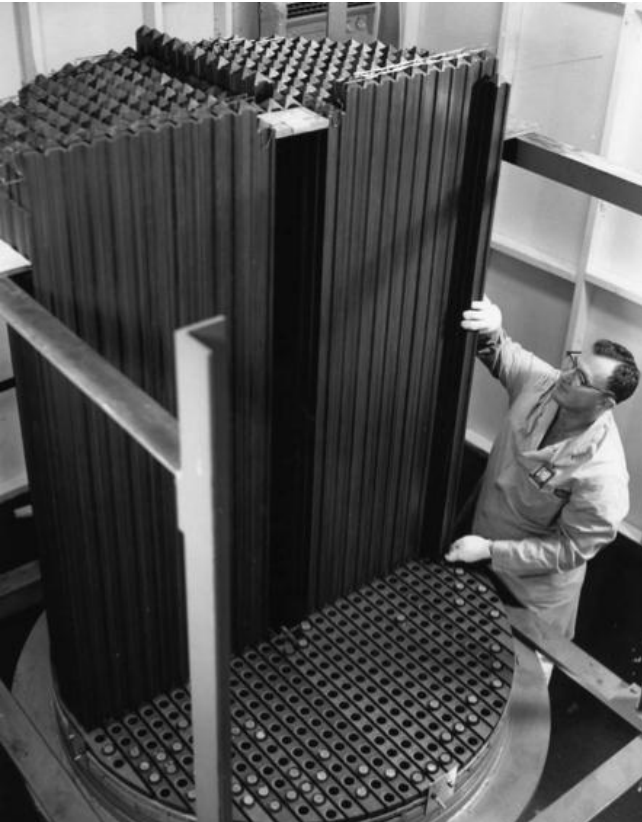
\includegraphics[width=0.75\textwidth]{msre_view.png}
  \caption{The \gls{MSRE} core, shown while being assembled, contained 1.95 m$^3$ of reactor graphite. The 1,140 fuel channels contain about 0.57m$^3$ of fuel salt.}
  \vspace{-0.6em}
  \label{fig:msre}
\end{figure}
\FloatBarrier

Once \gls{MSRE} began operating, most research and development work on \glspl{MSR} was in support of the \gls{MSRE}. Therefore, molten fluoride salt chemistry continued developing during this period. Vacuum distillation at high temperatures (1000$^{\circ}$C) successfully separated lithium fluoride and beryllium fluoride from rare earths \cite{kelly_removal_1965}. This method provided an inexpensive, on-site way for recovering valuable rare materials, and following this, the efforts for future reactors changed focus to a two-fluid breeder. In this reactor, the fuel salt should be fluorinated to recover the uranium and distilled to separate carrier salt from fission products. The blanket salt must be processed by fluorination alone because few fission happens in the blanket, consequently, fission products do not accumulating there \cite{rosenthal_molten-salt_1970}. Graphite tubes in the core prevented the fissile and fertile streams from mixing.

Two-fluid system analyses have shown that the breeding ratio could be in the range of 1.07 to 1.08, which with low fissile inventory would lead to relatively good fuel utilization. Consequently, the development effort for future molten salt reactors by \gls{ORNL} was aimed mainly at the features of two-fluid breeders \cite{briggs_summary_1967}. The main drawback of those reactors was identified as short graphite pipes lifetime due to neutron flux damage. Figure~\ref{fig:two_fluid} demostrates design of two-fluid \gls{MSBR} single cell.

Later, in 1967, new experimental information obtained from \gls{MSRE} and an advance in core design shifted the \gls{ORNL} molten salt program R\&D focus from the two-fluid to a single-fluid breeder. Part of the information influencing this change concerned the behavior of graphite at higher radiation exposures than had been achieved previously. To use reactor graphite type which was tested during \gls{MSRE} in \gls{MSBR}, lower core power densities enabled acceptable graphite lifetime but, even still, these components required frequent replacement. Furthermore, due to core assembly complexity, the entire core and reactor vessel required replacement when any graphite element reached its irradiation limit or developed a leak \cite{rosenthal_molten-salt_1970}.

To achieve an acceptable breeding ratio in single-fluid reactor, $^{233}$Pa ($\tau_{1/2}$= 27.4d) must be separated from the fuel salt and held outside the core until it decays to $^{233}$U. Laboratory experiments demonstrated a liquid-liquid extraction process for removing protactinium and uranium from molten fluoride salts. The method is to exchange thorium and lithium dissolved in molten bismuth for the components to be removed from the salt. Additional data have confirmed that the uranium can be selectively separated from the salt, the protactinium can be trapped in the salt in a decay tank, and the uranium can be returned back to the fuel salt by electrolysis for subsequent transfer to the core. Analysis indicated that the extraction and electrolysis could be carried out rapidly and continuously.

The fertile ``blanket'' in the single-fluid breeder is obtained by increasing the volume fraction of fuel salt and reducing the volume fraction of graphite in the outer part of the reactor. This advanced core design makes the outer region undermoderated and increases neutron capture there by the $^{232}$Th. Moreover, most neutrons are born in the inner region, at some distance from the reactor boundary, and captures in the outer region reduce the neutron leakage. Further studies indicated that fuel utilization in single-fluid, two-region \gls{MSR} can be as good as in two-fluid prototype, and even with the limitation on graphite lifetime, the economics might be better \cite{rosenthal_molten-salt_1970}. Thus, in 1968 \gls{ORNL} the \gls{MSR} Program was oriented toward the development of single-fluid breeder reactor.

Despite the success of \gls{ARE} and \gls{MSRE}, the \gls{MSR} program closed down in the early 1970s in favor of the liquid metal fast-breeder reactor (LMFBR) \cite{macpherson_molten_1985}, after which molten salt reactor research stagnated in the United States. As of 2018, the \gls{ARE} and \gls{MSRE} remain the only \glspl{MSR} ever operated in the world.

Recently, interest in \glspl{MSR} has returned, with multiple new companies pursuing commercialization of \gls{MSR} designs (e.g. liquid-fueled molten salt designs from Transatomic \cite{transatomic_power_corporation_technical_2016}, Terrapower, Terrestrial \cite{leblanc_18_2017}, and Thorcon \cite{jorgensen_19_2017}). China initiated a thorium molten salt reactor research project, and demonstrations of the liquid fuel version (TMSR-LF) are targeted for 2024 \cite{dai_17_2017}. European Union funds the Safety Assessment of the Molten Salt Fast Reactor (SAMOFAR) project, in which several European research institutes and universities are developing various molten salt reactor prototypes such as the \gls{MSFR} \cite{fiorina_molten_2013}, the \gls{MOSART} \cite{ignatiev_molten_2014}.
To further develop of these \gls{MSR} concepts, particularly with respect to their strategies for online reprocessing and refueling, computational analysis methods capturing their unique reactor physics and process chemistry are needed.

\begin{figure}[htp!] % replace 't' with 'b' to 
  \centering
  \vspace{-0.3em}
  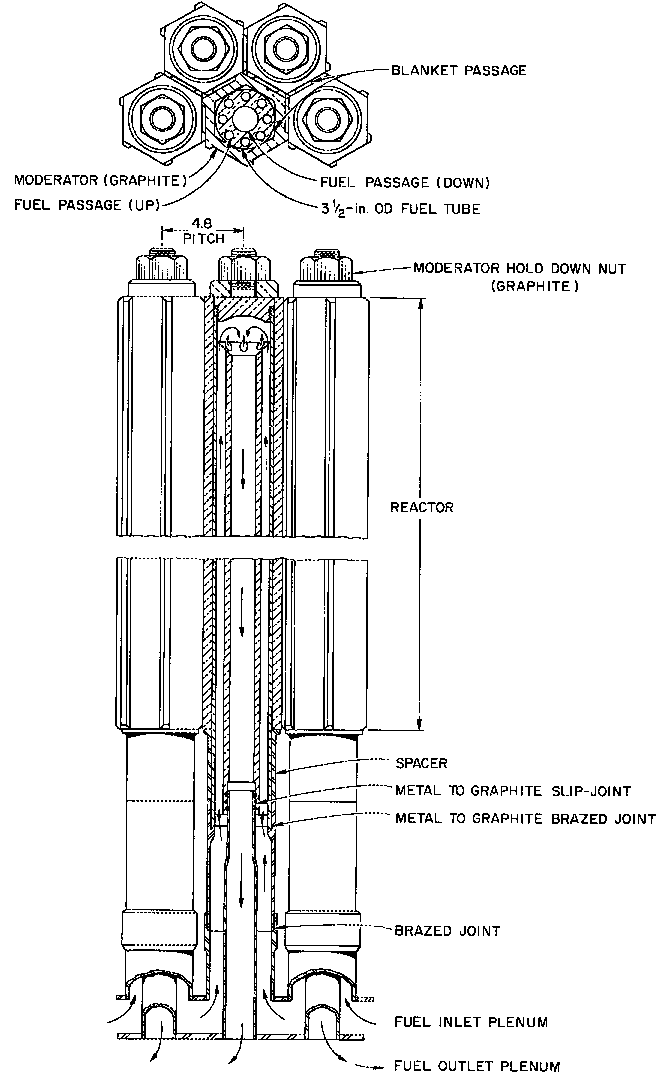
\includegraphics[width=0.85\textwidth]{two_fluid.png}
  \caption{A single graphite ``fuel cell" for a two-fluid molten-salt breeder reactor. Fuel salt flowed upward from the entrance plenum through eight channels at 45-degree angles to one another, then downward through the central channel to the exit plenum \cite{briggs_molten-salt_1966}.}
  \vspace{-0.6em}
  \label{fig:two_fluid}
\end{figure}
\FloatBarrier

\section{Thorium fuel cycle overview}
In the early days of nuclear energy industry, in the United States as a follow-up of the Manhattan Project (1945-1960), leading U.S. national laboratories studied thorium as a possible substitute for uranium and the possibilty of using $^{233}$U in a nuclear weapon. In the Atoms for Peace Program, with its great variety of developments (1955-1975), thorium appeared to be an interesting resource for supplementing limited uranium availability in the context of a fast-growing nuclear industry because thorium is  at least 4-5 times more abundant than uranium in Earth`s crust and preparation of thorium fuel does not require difficult and expensive enrichment processes. The International Fuel Cycle Evaluation Conference (INFCE) of 1978 predicted thorium would someday rival uranium in importance. It stated that in case of the optimistic nuclear energy development scenario, thorium would be called upon massively in the future. These predictions were too optimistic. However, in the long term, the use of thorium along with uranium could improve the potential of nuclear energy \cite{lung_perspectives_1998}.

During this pioneering period, thorium fuel cycle research and development for prototype demonstration reactors began, first in the United States under cooperation between the United States Atomic Energy Commission (USAEC) and U.S. industry, then in Europe. About 1500 kg of $^{233}$U have been bred in the United States from 900 metric tons of thorium. Many reactor prototypes as well as thorium extraction plants were built and operated in many countries. The U.S. and France have milled about 2000 metric tons of thorium, part of which is still available \cite{lung_perspectives_1998}. However, for most countries uranium is abundant and research in thorium fuel cycles diminished from late 1970s to 2000s. A notable exception was India's three-stage nuclear power program \cite{natarajan_fast_2007}. In the twenty-first century, thorium's potential for improving waste characteristics is generating renewed interest in the thorium fuel cycle \cite{bagla_thorium_2015}.

Natural thorium is almost exclusively composed of $^{232}$Th. Figure~\ref{fig:th_cycle} shows the breeding schemes for Uranium-Plutonium and Thorium-Uranium fuel cycles. In the Uranium-Plutonium cycle, production of fissile material ($^{239}$Pu) in a fast-spectrum reactor occurs by neutron irradiation of fertile material ($^{238}$U), while in the thorium fuel cycle $^{232}$Th absorbs a neutron in either a fast or thermal reactor. Next, the $^{233}$Th emits an electron and an anti-neutrino by $\beta^-$ decay to become $^{233}$Pa. The protactinium then emits another electron and anti-neutrino by a second $\beta^-$ decay to become $^{233}$U, which in turn is used as fuel. In most \gls{MSR} designs, the $^{233}$Pa is extracted and protected from neutrons (to prevent the core's poisoning via the $^{233}$Pa transmutation into $^{234}$Pa and then to $^{234}$U), until it has decayed to $^{233}$U. Figure~\ref{fig:th_cycle} demonstrates transmutations in the thorium and U-Pu fuel cycles. This is done in order to improve the breeding ratio which is low compared to fast reactors. 

\begin{figure}[t] % replace 't' with 'b' to 
  \centering
  \vspace{-0.3em}
  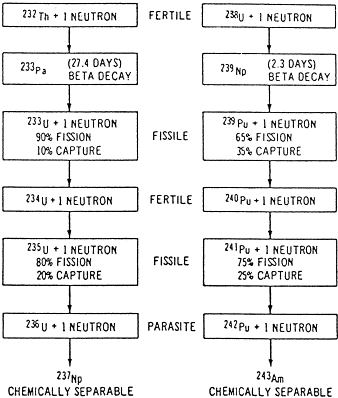
\includegraphics[width=0.70\textwidth]{th_u_cycle.png}
  \caption{Isotopic build-up in $^{232}$Th and $^{238}$U breeding systems \cite{eschbach_possible_1966}.}
  \vspace{-1.1em}
  \label{fig:th_cycle}
\end{figure}
\FloatBarrier

Although the thermal neutron fission cross section ($\sigma_f$) of the resulting $^{233}$U is comparable to $^{235}$U and $^{239}$Pu, it has a much lower capture cross section ($\sigma_c$) than other two fissile isotopes, providing fewer non-fissile neutron absorptions and improving neutron economy. Figure~\ref{fig:n_yeild} shows thermal utilization factor ($\eta$) which in $^{233}$U is greater than other two over a wide range of energies, including the thermal spectrum. Consequently, thorium fuels can be the basis for a thermal breeder reactor \cite{iaea_thorium_2005}, while a breeding reactor in the U-Pu cycle requires a fast neutron spectrum, because, in the thermal spectrum, one neutron absorbed by $^{239}$Pu in average produces less than two neutrons.

Another advantage of the thorium fuel cycle is inherent proliferation resistance due to contamination of fissile $^{233}$U with $^{232}$U. $^{232}$U cannot be chemically separated from $^{233}$U and  emits high-energy gamma radiation. These high-energy $\gamma$-rays are a radiological hazard, thus, remote handling is necessary for separated uranium and such materials could be passively detected.

\begin{figure}[htbp!] % replace 't' with 'b' to 
  \centering
  \vspace{-0.3em}
  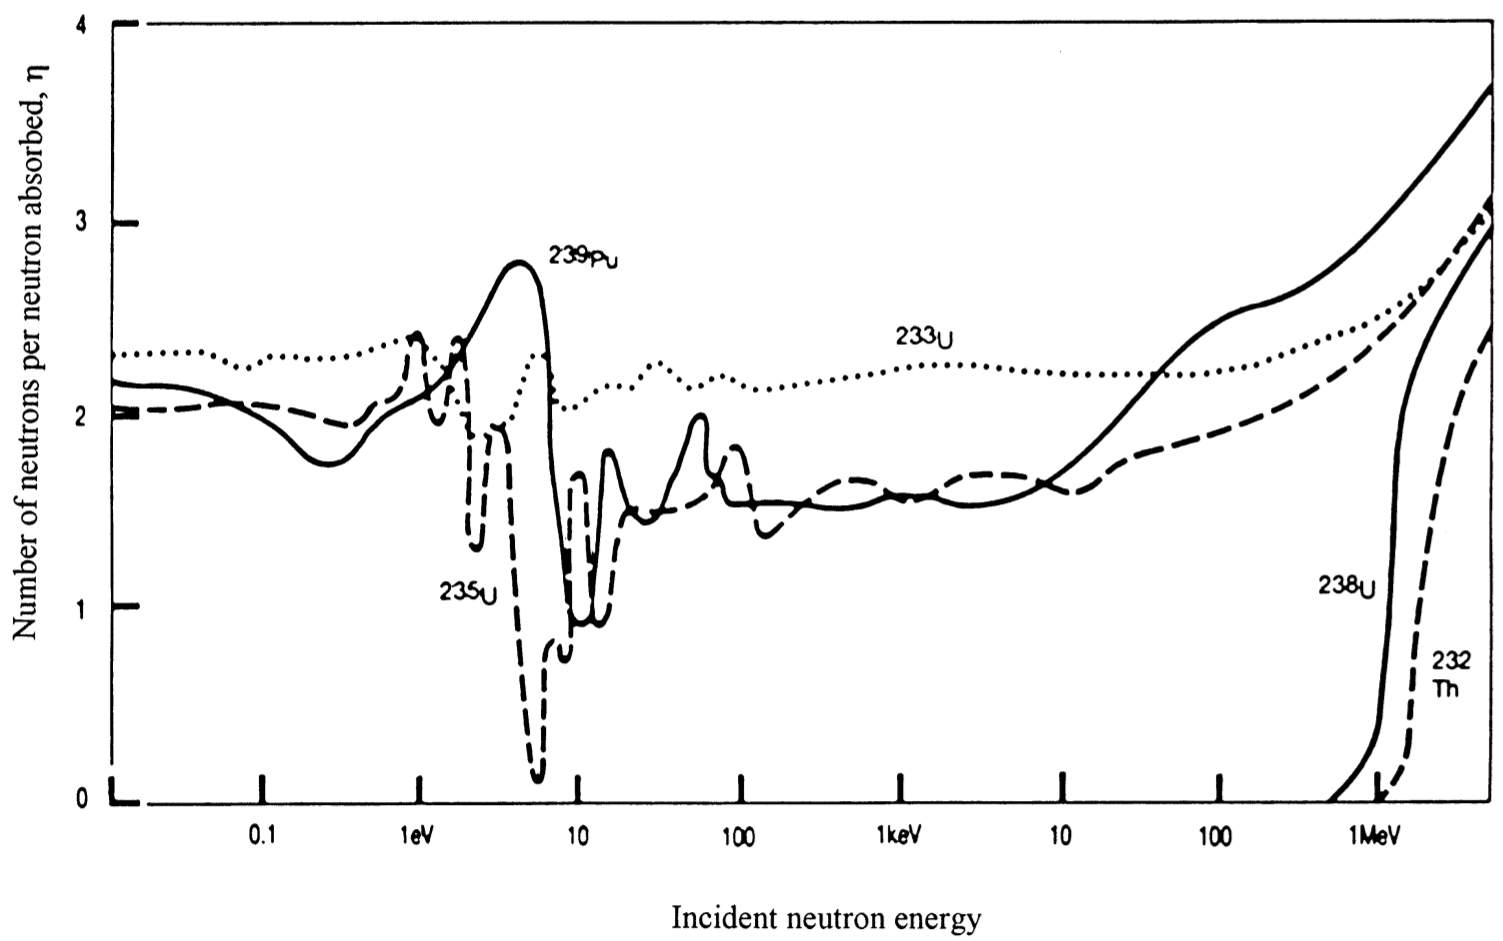
\includegraphics[width=\textwidth]{neutron_yeild.png}
  \caption{Neutron yield per neutron absorbed \cite{anon_plutonium_1989}.}
  \vspace{-1.1em}
  \label{fig:n_yeild}
\end{figure}
\FloatBarrier

Moreover, from the respective positions of uranium and thorium in the periodic table, the long-lived minor actinides resulting from fission are in much lower quantity in the thorium cycle, especially compared with the uranium-plutonium cycle. Because of this, thorium is a potentially attractive alternative to uranium in \gls{MOX} fuels to minimize the generation of long-lived transuranic elements and maximize the destruction of plutonium.

For the many reasons explained above, the thorium fuel cycle has so far not been able to compete on par with uranium, which currently dominates nuclear energy. The time has come to have another hard look at what was perhaps too quickly set aside forty years ago and restart with new advanced computational methods. 

\section{Literature review}
Most contemporary nuclear reactor physics software is unable to perform depletion calculations in an online reprocessing regime. Furthermore, no established tool for liquid-fueled \gls{MSR} neutronics and fuel cycle evaluation exist, though internally developed tools from universities and research institutions can approximate online refueling \cite{serp_molten_2014}. The foundation for these tools was based on early \gls{MSR} simulation methods at \gls{ORNL}, which integrated neutronic and fuel cycle codes (i.e., ROD \cite{bauman_rod:_1971}) into operational plant tools (i.e., MRPP \cite{kee_mrpp:_1976}) for \gls{MSR} and reprocessing system design. More recent research efforts in Europe and Asia mainly focus on fast spectrum reactor fuel cycle analysis and couple external tools to neutron transport and depletion codes take into account continuous feeds and removals in \glspl{MSR}. Four of these efforts are listed in table~\ref{tab:fs_codes}.

\begin{table}[h!]
\centering
\caption{Tools and methods for fast spectrum system fuel cycle analysis.}
  \vspace{-0.8em}
\begin{tabular}{ |m{0.01\textwidth}|m{0.2\textwidth}|m{0.15\textwidth}|m{0.33\textwidth}|m{0.13\textwidth}|} 
\hline
\# & Neutronic code  & Depletion code    & \qquad Authors & Spectrum   \\[3pt]
\hline
1 & \gls{MCNP} \cite{noauthor_mcnp_2004}      & REM \cite{heuer_simulation_2010}  & Doligez \emph{et al.}, 2014; Heuer \emph{et al.}, 2014  \cite{doligez_coupled_2014,heuer_towards_2014}    & fast \\[5pt]
\hline
2 & ERANOS \cite{ruggieri_eranos_2006}      & ERANOS     & Fiorina \emph{et al.}, 2013 \cite{fiorina_investigation_2013}            & fast \\[5pt]
\hline
3 & KENO-IV \cite{goluoglu_monte_2011}     & ORIGEN \cite{gauld_isotopic_2011}     & Sheu \emph{et al.}, 2013 \cite{sheu_depletion_2013} & fast \\[5pt]
\hline
4 & SERPENT 2 \cite{leppanen_serpent_2015}   & SERPENT 2  & Aufiero \emph{et al.}, 2013 \cite{aufiero_extended_2013} & fast \\[5pt]
\hline
5 & MCODE \cite{xu_mcode_2008}      & ORIGEN2 \cite{croff_users_1980}      & Ahmad \emph{et al.}, 2015 \cite{ahmad_neutronics_2015}   & thermal  \\[5pt]
\hline
6 & \gls{MCNP}6     & CINDER90 \cite{goorley_mcnp6_2013}     & Park \emph{et al.}, 2015; Jeong \emph{et al.}, 2016 \cite{park_whole_2015, jeong_equilibrium_2016}& thermal\\[5pt]
\hline
7 & SCALE \cite{bowman_scale_2011}      & SCALE/ ChemTriton \cite{powers_new_2013}    & Powers \emph{et al.}, 2014; Betzler \emph{et al.}, 2017 \cite{powers_new_2013,powers_inventory_2014,betzler_molten_2017}& thermal\\[5pt]
\hline
8 & SERPENT 2      & SERPENT 2     & Rykhlevskii \emph{et al.}, 2017 \cite{rykhlevskii_online_2017} & thermal\\[5pt]
\hline
9 & \gls{MCNP}      & REM  & Nuttin \emph{et al.} \cite{nuttin_potential_2005}&thermal  \\[5pt]
\hline
\end{tabular}
  \vspace{-1.1em}
  \label{tab:fs_codes}
\end{table}

Most of these methods are also applicable to thermal spectrum reactors. Additional tools developed specifically for thermal \gls{MSR} applications are also listed in table~\ref{tab:fs_codes}.

Methods (1, 3, 4) provide some form of reactivity control, and methods (1, 4, 5, 6, 8, 9) use a set of all nuclides in depletion calculations. 

Liquid-fueled \gls{MSR} designs have online separations and/or feeds, where material is moved to or from the core at all times (continuous) or at specific time steps (batch). To account for batch discharge, a depletion tool must remove some or all material at specified intervals. This requires the burn-up simulation to stop at a given time and restart with a new liquid fuel composition (after removal of discarded materials and addition of fissile/fertile materials). Accounting for a continuous removal or addition is more difficult because it requires adding a term to the Bateman equations. In SCALE \cite{bowman_scale_2011}, ORIGEN \cite{gauld_isotopic_2011} solves a set of Bateman equations using spectrum-averaged fluxes and cross sections generated from a deterministic transport calculation. Methods (1, 4, 8) model true continuous feeds and removals, while other methods employ a batch-wise approach. \gls{ORNL} researchers have developed ChemTriton, a Python-based script for SCALE/TRITON which uses a semi-continuous batch process to simulate a continuous reprocessing. This tool models salt treatment, separations, discharge, and refill using a unit-cell \gls{MSR} SCALE/TRITON model over small time steps to simulate continuous reprocessing and deplete the fuel salt \cite{powers_new_2013}.

Thorium-fueled \gls{MSBR}-like reactors similar to the one in this thesis are described in (6, 7, 8, 9). Nevertheless, most of these efforts considered only simplified unit-cell geometry because depletion computations for a many-year fuel cycle are computationally expesive even for simple models. 

Nuttin \emph{et al.} broke up reactor core geometry into tree \gls{MCNP} cells: one for salt channels, one for two salt plena above and below the core and the last cell for the annulus, consequently, two-region reactor core was approximated by one region with averaged fuel/moderator ratio \cite{nuttin_potential_2005}.  A similar approach was used by Powers \emph{et al.}, Betzler \emph{et al.}, and Jeong \emph{et al.} \cite{powers_new_2013,powers_inventory_2014,betzler_modeling_2016, betzler_molten_2017, jeong_development_2014, jeong_equilibrium_2016} and clearly misrepresent the two-region breeder reactor concept. The unit-cell or one-region models may produce reliable results for homogeneous reactor cores (i.e. \gls{MSFR}, \gls{MOSART}) or for one-region single-fluid reactor designs (i.e. \gls{MSRE}). A two-region \gls{MSBR} must be simulated using a whole-core model to represent different neutron transport in the inner and outer regions of the core, because most fissions happens in the inner region while breeding occurs in the outer zone.  

Aufiero \emph{et al.} extended the Monte Carlo burnup code SERPENT 2 and employed it to study the material isotopic evolution of the \gls{MSFR}. The developed extension directly takes into account the effects of online fuel reprocessing on depletion calculations and features a reactivity control algorithm. The extended version of SERPENT 2 was assessed against a dedicated version of the deterministic ERANOS-based EQL3D procedure \cite{ruggieri_eranos_2006} and adopted to analyze the \gls{MSFR} fuel salt isotopic evolution. We employed this extended SERPENT 2 for a simplified unit-cell geometry of thermal spectrum thorium-fueled \gls{MSBR} and obtained results which contradict existing \gls{MSBR} depletion simulations \cite{jeong_equilibrium_2016}.

Chapter 3 and 4 of the current study are similar to the works described in (6, 7, 9), but the focus of this work is on developing new external open-source tool for online reprocessing simulation: SaltProc. The tool works with the SERPENT 2 Monte Carlo software, and has a reactivity control module which allows reactivity adjustment by changing feed material flow to avoid control rod movement. Moreover, this work extends recent research efforts by simulating online reprocessing with a high-fidelity, full-core 3-D model without any approximations in the core geometry.

Another challenge presented by liquid-fueled systems is the fuel material movement. Fuel flow is important because of delayed neutron emission. In a reactor with solid fuel, the delayed neutron precursor fission products remain very close to the location where fission happened, emitting delayed neutrons at that location. Delayed neutrons have softer energy spectrum than prompt neutrons and their effective delayed neutron fraction $\beta_{eff}$ enables reactor control on human time scales \cite{betzler_molten_2017}. This quantity has significant impact on reactor safety because delayed neutron production occurs on a relatively long time frame and enables control of the reactor. In case of liquid-fuled reactors the precursors drifting, consequently, the fission and delayed neutron emission locations are different. The reactor design determines the effect of the precursor drift on the core physics. The flow parameters (e.g., flow rate, pipe diameter, primary loop length) affect the effective delayed neutron fraction $\beta_{eff}$. Hence, to take into account tightly coupled \gls{MSR} neutronics, thermal-hydraulics, and precursor drift, a multi-physics code is required.

There are number of multi-physics tools which successfully describe steady-state and transient behavior of various \gls{MSR} concepts. Krepel \emph{et al.} extended the \gls{LWR} diffusion code DYN3D to consider drift of delayed neutron precursors alongside the reactor temperature profile, re-introducing the extended code as DYN3D-MSR \cite{krepel_dyn3d-msr_2007}. That work compared DYN3D-MSR against experimental \gls{MSRE} data to simulate local fuel channel blockage accidents as well as local temperature perturbations.

Similarly, Kophazi \emph{et al.} used iterative coupling between the three-dimen\-sional and the one-dimensional heat conduction model DALTON neutronic and neutronic model to analyze normal \gls{MSRE} operation as well as channel-blocking-incident transients \cite{kophazi_development_2009}. The Kophazi model added entrance effects of heat transfer coefficients as well as thermal coupling between fuel channels through moderator heat conduction. Later, Cammi \emph{et al.} performed a 2D-axisymmetric single-channel analysis of the \gls{MSBR} using the commercial finite element package COMSOL Multiphysics \cite{cammi_multi-physics_2011}. That work directly solved the fuel salt velocity field, and used heterogeneous group constants in fuel and moderator regions.  

More recently, Aufiero \emph{et al.} \cite{aufiero_development_2014} approached transient simulations in the \gls{MSFR} with the finite volume OpenFOAM multiphysics toolkit \cite{weller_tensorial_1998}.  This approach benefits from pre-implemented turbulence models available in the OpenFOAM library and captures the full-core three-dimensional geometry of the reactor primary circuit.  OpenFOAM \gls{CFD} has additionally been shown by Laureau \emph{et al.} \cite{laureau_transient_2017} to couple well with Transient Fission Matrix neutronics within the \gls{MSFR} \cite{laureau_transient_2015}.

Concurrently, Lindsay \emph{et al.} have introduced Moltres, a physics application for multiphysics modeling of liquid-fueled \glspl{MSR} \cite{lindsay_introduction_2018}. It couples equations for neutron diffusion, thermal-hydraulics, and delayed neutron precursor transport. Moltres solves arbitrary-group neutron diffusion, temperature, and precursor governing equations in one to three dimensions, and can be deployed on an arbitrary number of processing units. 2D-axisymmetric many-channel anlysis of the \gls{MSRE} in Moltres was successfully compared against experimental \gls{MSRE} data in steady-state mode.

In general, these research efforts use initial fuel salt composition, thus, considering the reactor core at the moment of startup. Nevertheless, fuel salt composition evolves significantly during fuel materials irradiation which leads to changes in the reactor neutronics. Chapter 5 of the present thesis introduces the equilibrium fuel salt composition and compare major reactor physics characteristics for both initial and equilibrium state. This results are necessarily for multi-physics analysis of accident transient scenarios for \gls{MSBR} using Moltres code for both fresh and irradiated fuel salt.


%\chapter[Steady-state full-core MSBR benchmark]{Steady-state full-core MSBR benchmark}

\section{SERPENT 2 code overview}
SERPENT is a continuous-energy Monte Carlo neutronics software capable of solving the neutron transport problem by tracking individual neutrons within the problem geometry and using stochastic method to determine chain of events for each neutron \cite{leppanen_serpent_2015}. SERPENT has been under active development at the VTT Technical Research Centre of Finland since 2004, where it was initially conceived as a tool to simplify group constant generation in a high-fidelity Monte Carlo environment. SERPENT is now widely used transport code  with a growing user base. Now SERPENT used by more than 500 registered individuals in 155 organizations located in 37 countries around the world. The burnup calculation capability in SERPENT is based on built-in calculation routines, without using any external solvers. A restart feature allows performing fuel shuffling or applying any modifications in the input by dividing the calculation into several parts, which is crucial for online reprocessing simulations.

The latest version, SERPENT 2, supports advanced geometries and has advanced burnup capabilities, including online refueling capabilities which are necessary for neutronic computations of pebble-bed reactors and liquid-fueled \glspl{MSR} \cite{aufiero_extended_2013}. Unfortunately, built-in online refueling features are still under active development and unavailable to ordinary users. Furthermore, recently multi-physics simulations using SERPENT 2 were demonstrated, i.e. coupled calculations with thermal-hydraulics, \gls{CFD} and fuel performance codes \cite{leppanen_numerical_2015}. Two-way coupling to thermal-hydraulics, \gls{CFD}, and fuel performance codes operates on two levels: internal coupling to built-in solvers for fuel behavior and thermal-hydraulics, and external coupling via a universal multi-physics interface. 

SERPENT 2 can be effectively run in parallel on computer clusters and multi-core workstations. Parallelization is handled by thread-based OpenMP, which has the advantage that all processsors use shared memory space. Calculations can be divided into several nodes by distributed-memory \gls{MPI} parallelization. SERPENT 2  is an improvement upon SERPENT 1, and contains a complete redesign of memory management using hybrid OpenMP \cite{dagum_openmp:_1998} + \gls{MPI} parallelization.  This hybrid parallelization is important in depletion calculations using computer clusters with multiple nodes, and allows to achieve significant speed-up in depletion calculations on computer clusters with more than 4'000 cores \cite{leppanen_serpent_2015-1}. 

All calculations presented in this thesis were performed using SERPENT 2 version 2.1.30 on Blue Waters’ XE6 nodes. For cross section generation, JEFF-3.1.2 nuclear data library was employed \cite{oecd/nea_data_bank_jeff-3.1.2_2014}. 

\section{Molten Salt Breeder Reactor description}
Figure~\ref{fig:ref_sect_msbr} shows the \gls{MSBR} vessel which has a diameter of 680 cm and a height of 610 cm. It contains a molten fluoride fuel-salt mixture that generates heat in the active core region and transports that heat to the primary heat exchanger by way of the primary salt pump. In the active core region, the salt flows through channels in moderating and reflecting graphite blocks. Salt at about 565$^{\circ}$C enters the central manifold at the bottom via four 40.64-cm-diameter nozzles and flows upward through channels in the lower plenum graphite. The fuel salt exits at the top at about 704$^{\circ}$C through four equally spaced nozzles which connect to the salt-suction pipes leading to primary circulation pumps. The fuel salt drain lines connect to the bottom of the reactor vessel inlet manifold.

Since reactor graphite experiences significant dimensional changes due to neutron irradiation, the reactor core was designed for periodic replacement. The reference \gls{MSBR} design has an average core power density of approximately 6.666 W/g. Based on the irradiation experimental data from \gls{MSRE}, core graphite lifetime density is about 4 years and reflector graphite lifetime is 30 years \cite{robertson_conceptual_1971}.

\begin{figure}[htp!] % replace 't' with 'b' to 
  \centering
  \vspace{-0.3em}
  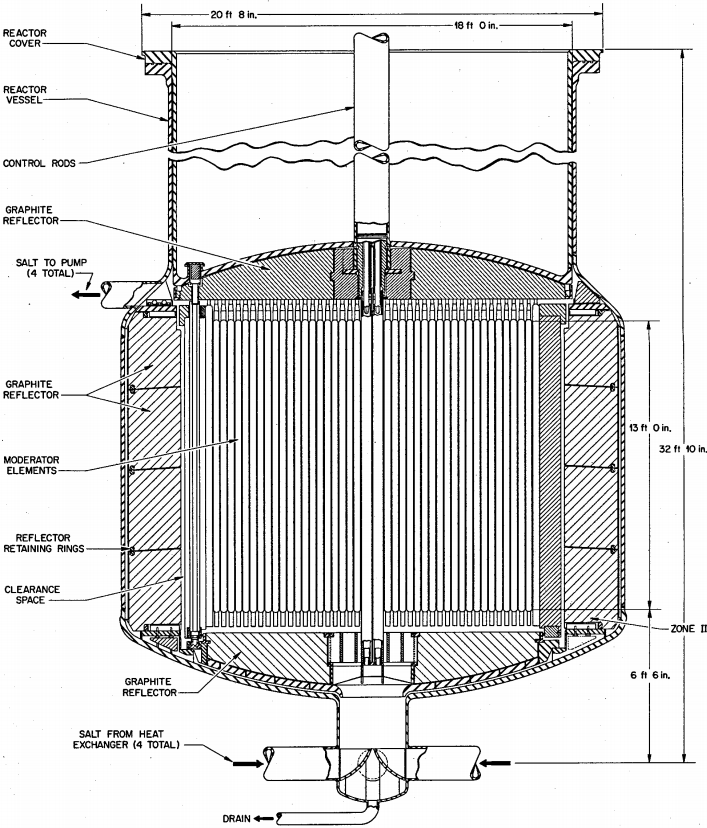
\includegraphics[width=\textwidth]{elev_view_vessel.png}
  \caption{Sectional elevation of \gls{MSBR} vessel \cite{robertson_conceptual_1971}.}
  \vspace{-0.6em}
  \label{fig:ref_sect_msbr}
\end{figure}

Moreover, it was decided to remove and install the core graphite as an assembly rather than by individual blocks, because it is relatively easier for maintenance personnel and has lower probability of radioactive elements escape due to used blocks damage during removal. In addition, handling the core as an assembly also allows the replacement core to be carefully preassembled and tested under factory conditions.

Figure~\ref{fig:ref_sect_msbr} and \ref{fig:ref_plan_msbr} demonstrate the configuration of the \gls{MSBR} vessel, core configuration, ``fission" (zone I) and ``breeding" (zone II) regions inside the vessel. The core has two radial zones bounded by a solid cylindrical graphite reflector and the vessel wall. The central zone, zone I, in which 13\% of the volume is fuel salt and 87\% graphite. Zone I composed of 1,320 graphite cells, 2 graphite control rods, and 2 safety\footnote{These rods needed for emergency shutdown only.} rods. The under-moderated zone, zone II, with 37\% fuel salt, and radial reflector, surrounds the zone I core region and serves to diminish neutron leakage. Zones I and II are surrounded radially and axially by fuel salt. This space for fuel is necessary for injection and flow of molten salt.

\begin{figure}[hbp!] % replace 't' with 'b' to 
  \centering
  \vspace{-0.3em}
  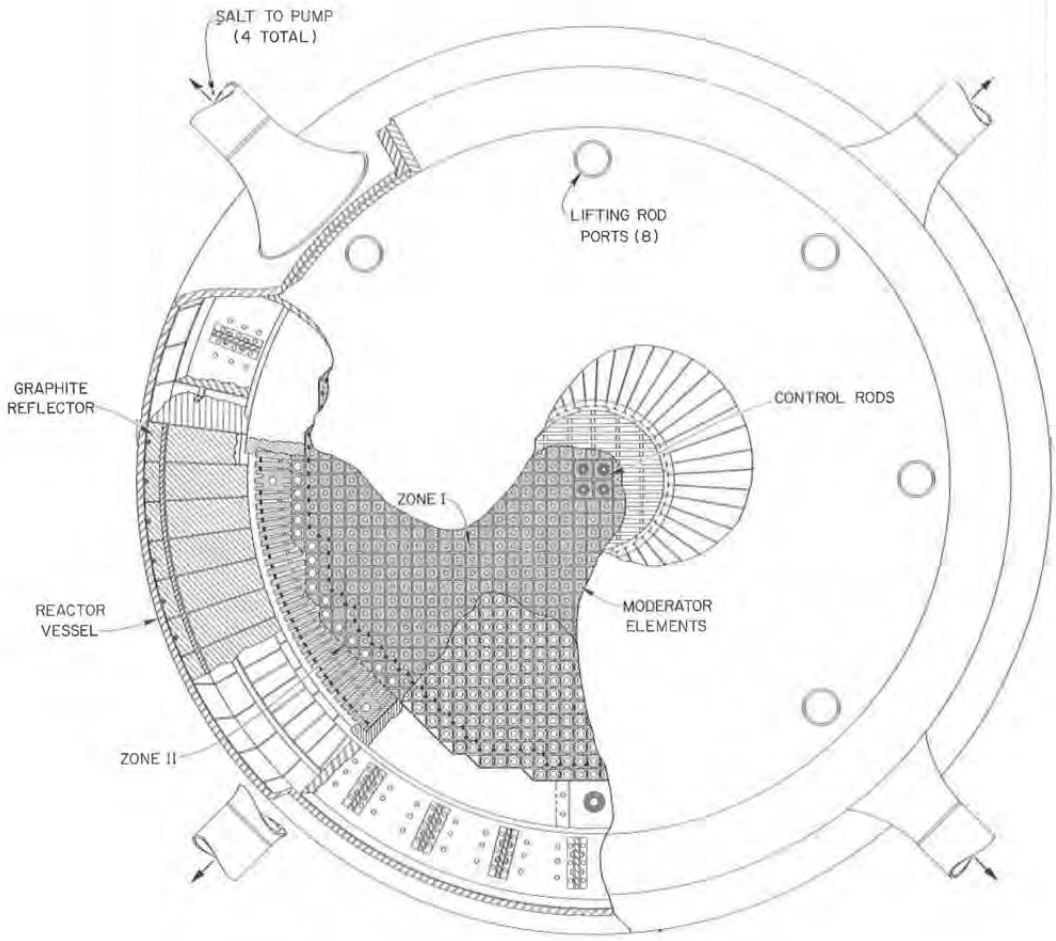
\includegraphics[width=\textwidth]{plan_view_vessel.png}
  \caption{Plan view of \gls{MSBR} vessel \cite{robertson_conceptual_1971}.}
  \vspace{-0.6em}
  \label{fig:ref_plan_msbr}
\end{figure}
\FloatBarrier

There are eight symmetric graphite slabs with a width of 15.24 cm in zone II, one of which is illustrated in Fig.~\ref{fig:detail_plan_view}. The holes in the centers are for the core lifting rods used during the core replacement operations. These holes also allow a portion of the fuel salt to flow to the top of the vessel for cooling the top head and axial reflector. Fig.~\ref{fig:detail_plan_view} also demonstrates the 5.08-cm-wide annular space between the removable core graphite in zone II-B and the permanently mounted reflector graphite. This annulus constists entirely of fuel salt, provides space for moving the core assembly, helps compensate the elliptical dimensions of the reactor vessel, and serves to reduce the damaging flux at the surface of the graphite reflector blocks.

\begin{figure}[hbp!] % replace 't' with 'b' to 
  \centering
  \vspace{-0.3em}
  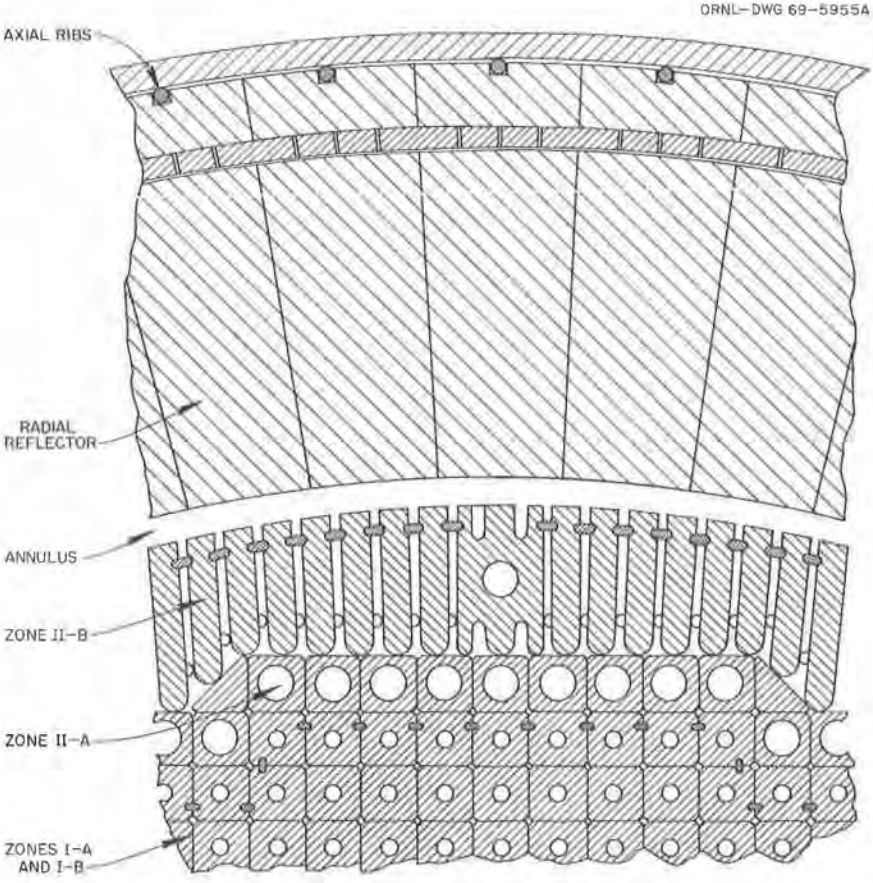
\includegraphics[width=\textwidth]{reflector_elements_ref.png}
  \caption{Detailed plan view of graphite reflector and moderator elements \cite{robertson_conceptual_1971}.}
  \vspace{-0.6em}
  \label{fig:detail_plan_view}
\end{figure}
\FloatBarrier

\subsection{Core zone I}
The central region of the core, called zone I, is made up of graphite elements, each $10.16$cm$\times$10.16cm$\times$396.24cm. In zone I, 13\% of the volume is fuel salt and 87\% is graphite. Zone I is composed of 1,320 graphite cells and 4 channels for control rods: two for graphite rods which both regulate and shim during normal operation, and two for backup safety rods consisting of boron carbide clad to assure sufficient negative reactivity for emergency situations.

These graphite elements have a mostly rectangular shape with lengthwise ridges at each corner that leave space for salt flow elements. Various element sizes reduce the peak damage flux and power density in the center of the core to prevent local graphite damage. Zone I is well-moderated to achieve the desired fission power density. Figure~\ref{fig:I_element_ref} demonstrates the elevation and sectional views of graphite elements of zone I \cite{robertson_conceptual_1971} and their SERPENT model \cite{rykhlevskii_full-core_2017}.

\subsection{Core zone II}
Zone II which is undermoderated, surrounds zone I. Combined with the bounding radial reflector, zone II serves to diminish neutron leakage. This zone is formed of two kinds of elements: large-diameter fuel channels (zone II-A) and radial graphite slats (zone II-B). 

Zone II has 37\% fuel salt by volume and each element has a fuel channel diameter of 6.604cm. The graphite elements for zone II-A are prismatic and have elliptical-shaped dowels running axially between the prisms and needed to isolate the fuel salt flow in zone I from that in zone II. Fig.~\ref{fig:II_element_ref} shows shape and dimensions of these graphite elements and their SERPENT model. Zone II-B elements are rectangular slats spaced far enough apart to provide the 0.37 fuel salt volume fraction. The reactor zone II-B graphite 5.08cm-thick slats vary in the radial dimension (average width is 26.67cm) as shown in figure~\ref{fig:detail_plan_view}. Zone II serves as a blanket to achieve the best performance: a high breeding ratio and a low fissile inventory. The neutron energy spectrum in zone II is made harder to enhance the rate of thorium resonance capture relative to the fission rate, thus limiting the neutron flux in the outer core zone and reducing the neutron leakage \cite{robertson_conceptual_1971}. 

\begin{figure}[hbp!] % replace 't' with 'b' to 
  \centering
  \vspace{-0.3em}
  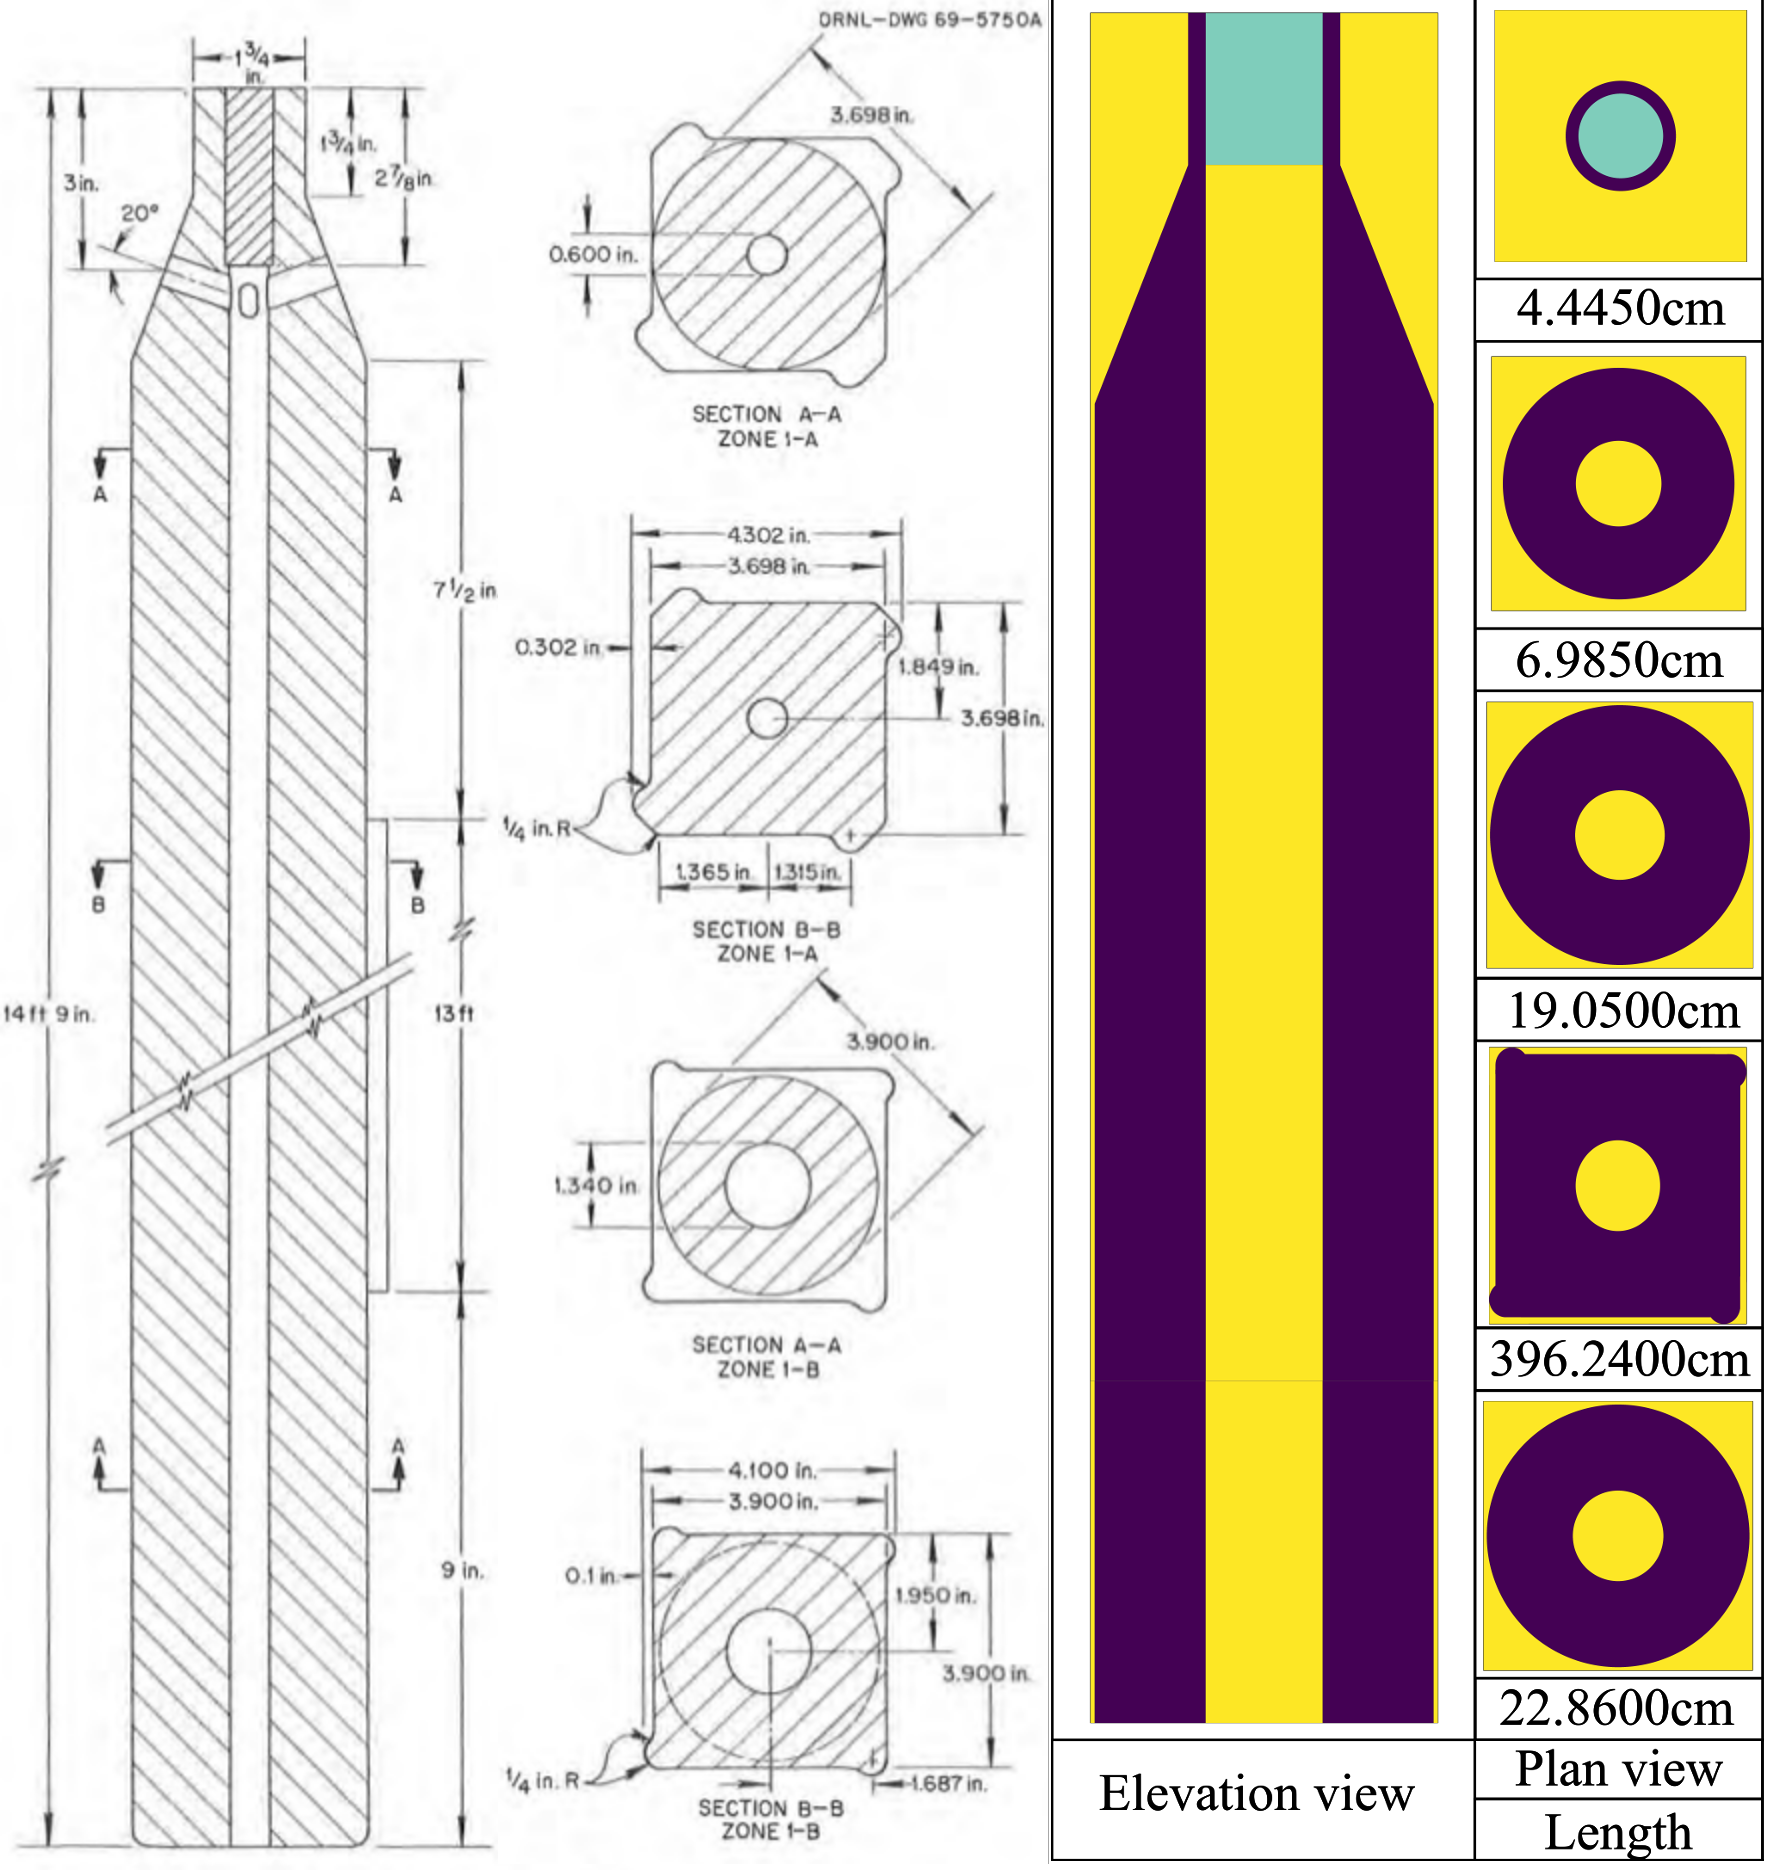
\includegraphics[width=\textwidth]{zone_I_element_ref.png}
  \caption{Graphite moderator elements for zone I \cite{robertson_conceptual_1971,rykhlevskii_full-core_2017}.}
  \vspace{-0.6em}
  \label{fig:I_element_ref}
\end{figure}
\FloatBarrier

\begin{figure}[hbp!] % replace 't' with 'b' to 
  \centering
  \vspace{-0.3em}
  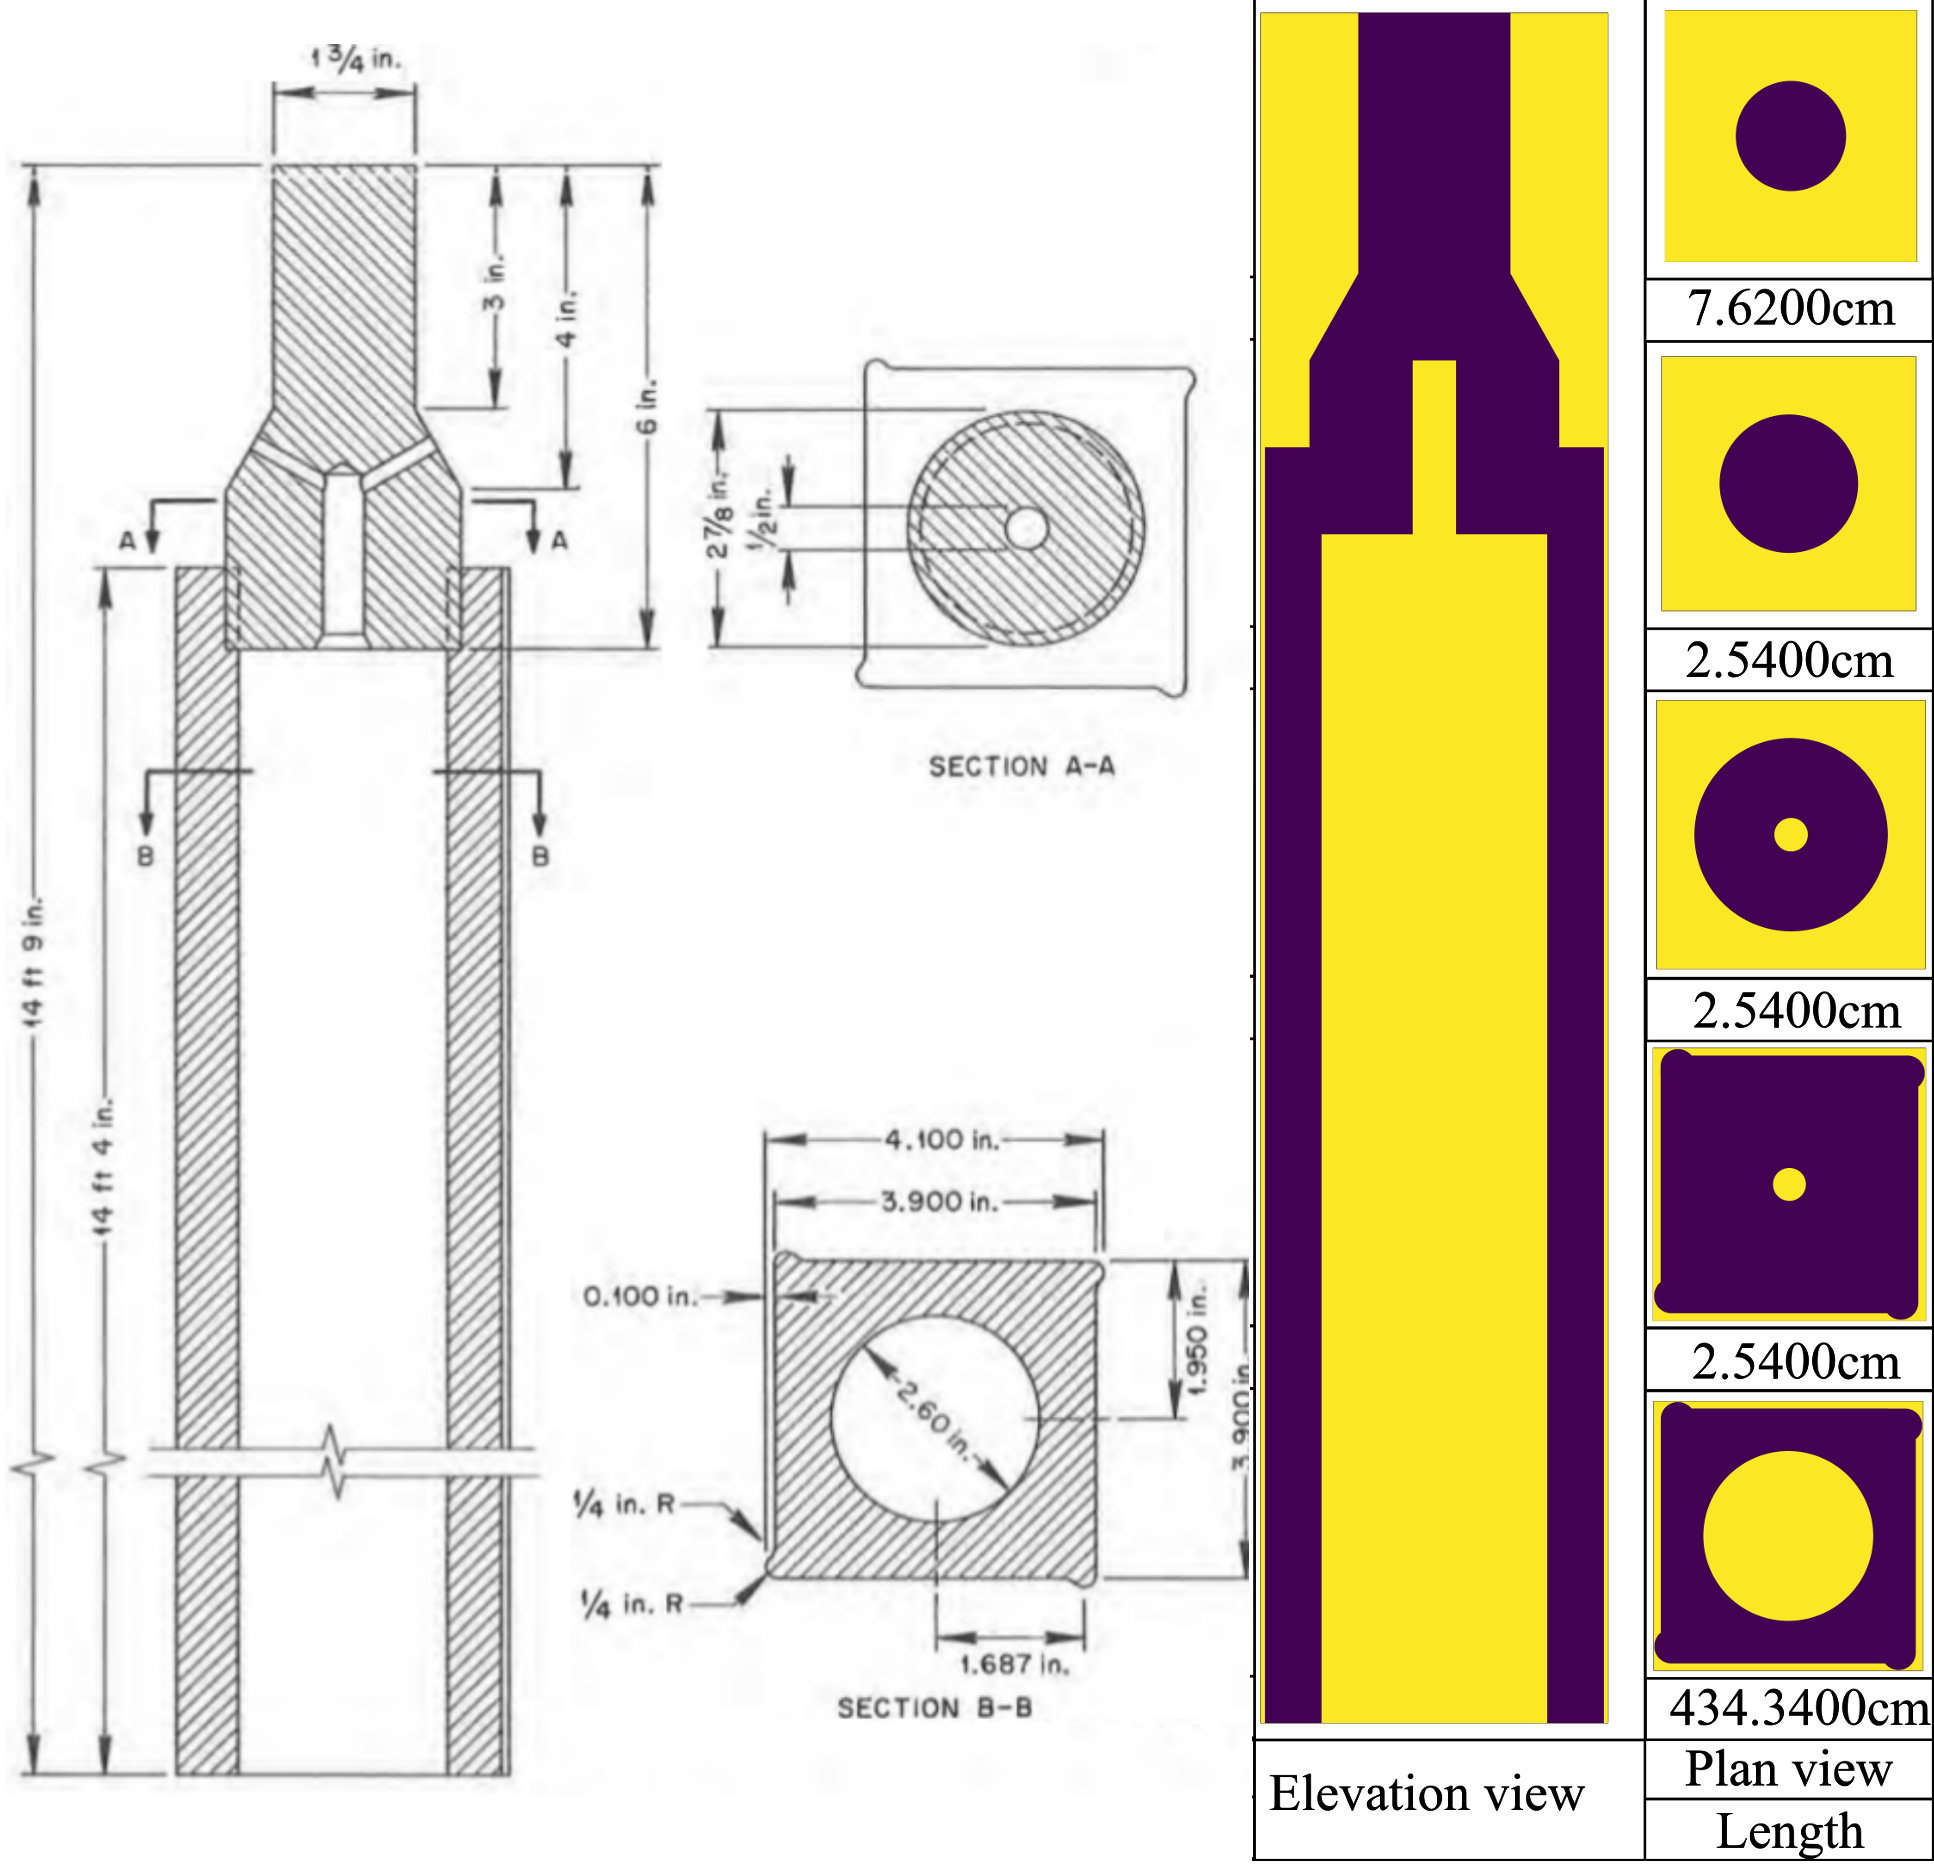
\includegraphics[width=\textwidth]{zone_II_element_ref.png}
  \caption{Graphite moderator elements for zone II-A \cite{robertson_conceptual_1971,rykhlevskii_full-core_2017}.}
  \vspace{-0.6em}
  \label{fig:II_element_ref}
\end{figure}
\FloatBarrier

\section{Existing full-core MSBR models}
There are few recent studies presenting full-core \gls{MSBR} models for neutronics analysis. Park \emph{et al.} developed an MCNP6 model for burnup computations and safety parameter analysis \cite{park_whole_2015}. This model has significant geometry simplifications in zone II-B graphite elements, and entirely neglects lengthwise ridges at each cell corner. Figure~\ref{fig:park} shows the simplifications in the model geometry.  More recently, Skirpan \emph{et al.} built a model of the core using Shift \cite{pandya_implementation_2016} to compare the fidelity of one-cell, two-cell and full-core models of the \gls{MSBR} \cite{skirpan_fuel_2017}. In this model, complex cell geometry in zone I and zone II-A were approximated to slightly rotated square cylinders (figure~\ref{fig:skirpan_cell}). Moreover, as can be seen from figure~\ref{fig:skirpan_plan}, zone II-B was described by Skirpan \cite{skirpan_fuel_2017} using horizontal, vertical and 45$^\circ$-degree graphite elements. These approximations distort neutron flux and reacton rates in that region, and, consequently, may misrepresent breeding parameters of the reactor.

Therefore, full-core Monte Carlo model with sufficient fidelity is necessary for online reprocessing and refueling simulation. Moreover, a high-fidelity model is essential for problem-oriented homogenized nuclear data (multi-group cross sections and diffusion constants) generation for deterministic reactor codes, and for coupled simulations.

\begin{figure}[hbp!] % replace 't' with 'b' to 
  \centering
  \vspace{-0.3em}
  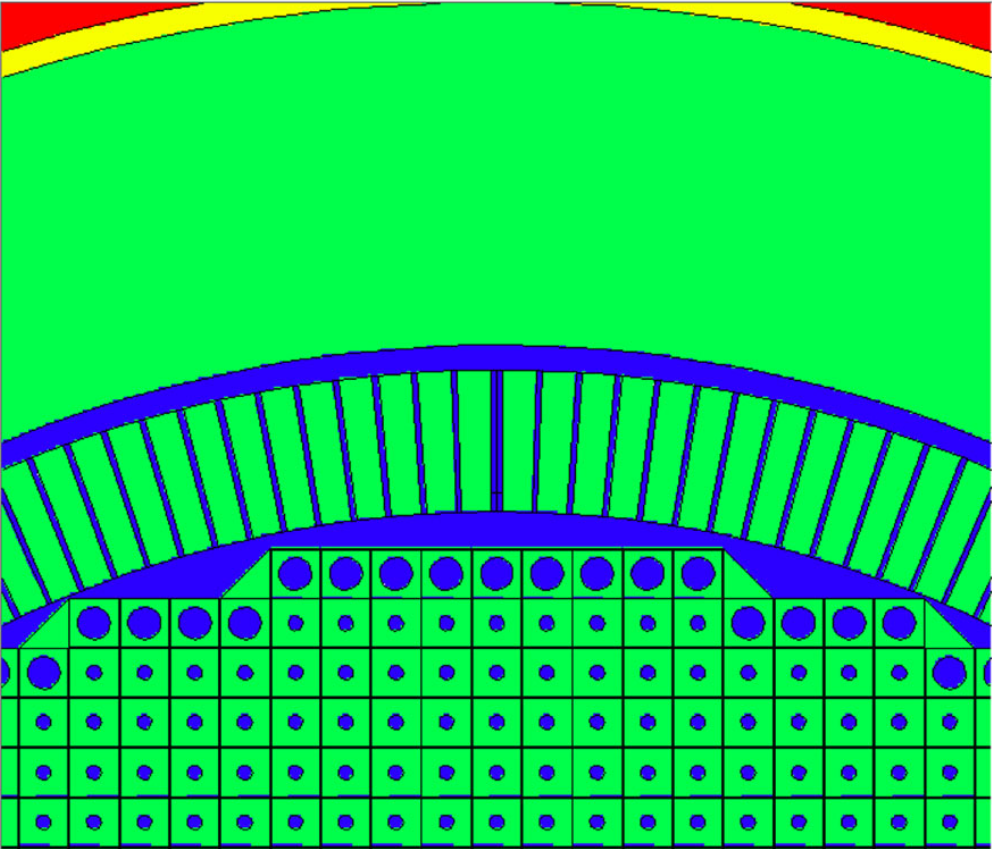
\includegraphics[width=\textwidth]{park_detailed_view.png}
  \caption{Graphite moderator elements  for zone II and reflector from Park \gls{MSBR} model (MCNP6) \cite{park_whole_2015}.}
  \vspace{-0.6em}
  \label{fig:park}
\end{figure}
\FloatBarrier

\begin{figure}[htp!] % replace 't' with 'b' to 
  \centering
  \vspace{-0.3em}
  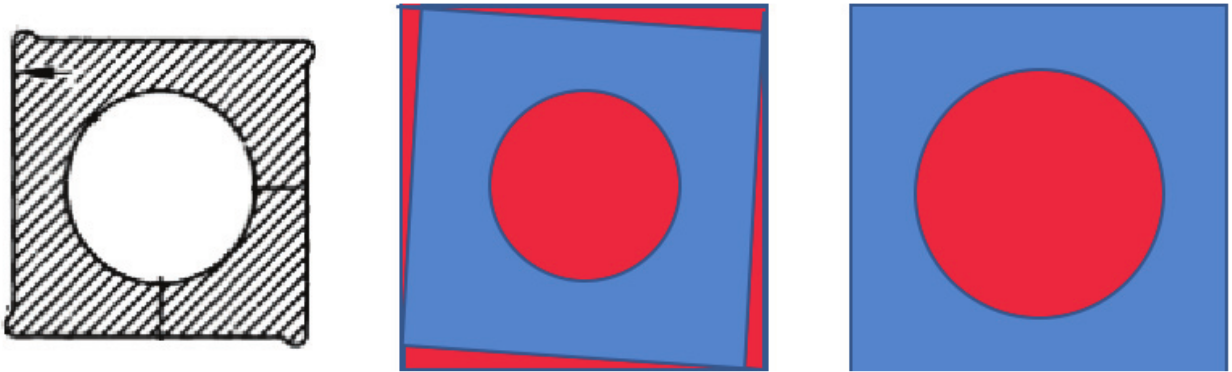
\includegraphics[width=0.95\textwidth]{skirpan_cell.png}
  \caption{Geometry of an MSBR fuel channel (left) approximated with a simple geometric model (center) to calculate appropriate volumes to reduce to a two-region model (right) from Skirpan model (Shift). Red is fuel salt, blue is graphite \cite{skirpan_fuel_2017}.}
  \vspace{-0.6em}
  \label{fig:skirpan_cell}
\end{figure}

\begin{figure}[hbp!] % replace 't' with 'b' to 
  \centering
  \vspace{-0.3em}
  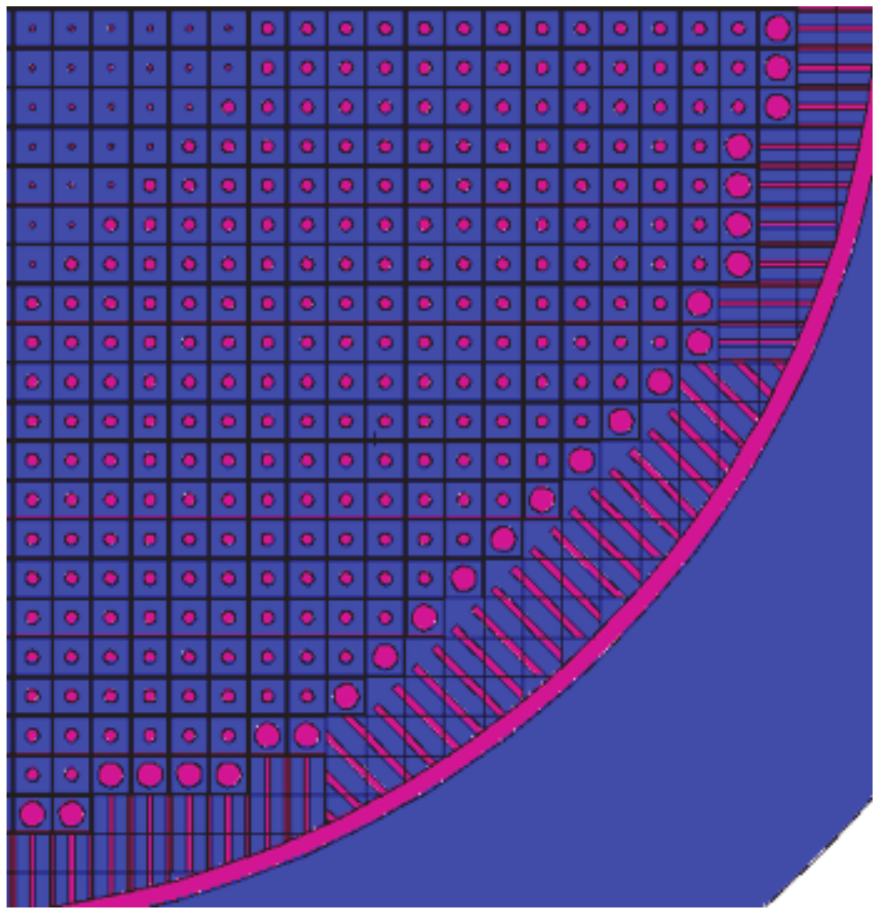
\includegraphics[width=0.7\textwidth]{skirpan_plan_view.png}
  \caption{Plan view of the \gls{MSBR} full-core transport model at core horizontal midplane from Skirpan model (Shift). Pink is fuel salt, blue is graphite \cite{skirpan_fuel_2017}.}
  \vspace{-0.6em}
  \label{fig:skirpan_plan}
\end{figure}
\FloatBarrier

\section{SERPENT 2 model}

Advanced geometry surfaces in SERPENT are employed to represent complex irregular \gls{MSBR} core. Fig.~\ref{fig:serpent_plan_view} shows the plan view of the whole-core configuration at the expected reactor operational level when both graphite control rods are fully inserted, and the safety rods are fully withdrawn. The safety rods only get inserted during an accident and were not inserted in this model. Another feature of the \gls{MSBR}, delayed neutron precursor drift corresponding to its circulating liquid fuel, is not treated here. 

Fig.~\ref{fig:serpent_sectional_view} shows the longitudinal section of the reactor. The violet color represents graphite, and the yellow represents fuel salt. The blue color shows Hastelloy-N, a material used for the plenum and vessel wall, and the white color is a void space. The model contains over 2000 geometric surfaces and 2066 calculation zones. In this thesis, all figures of the core were generated using the built-in SERPENT plotter.

\begin{figure}[hbp!] % replace 't' with 'b' to 
  \centering
  \vspace{-0.3em}
  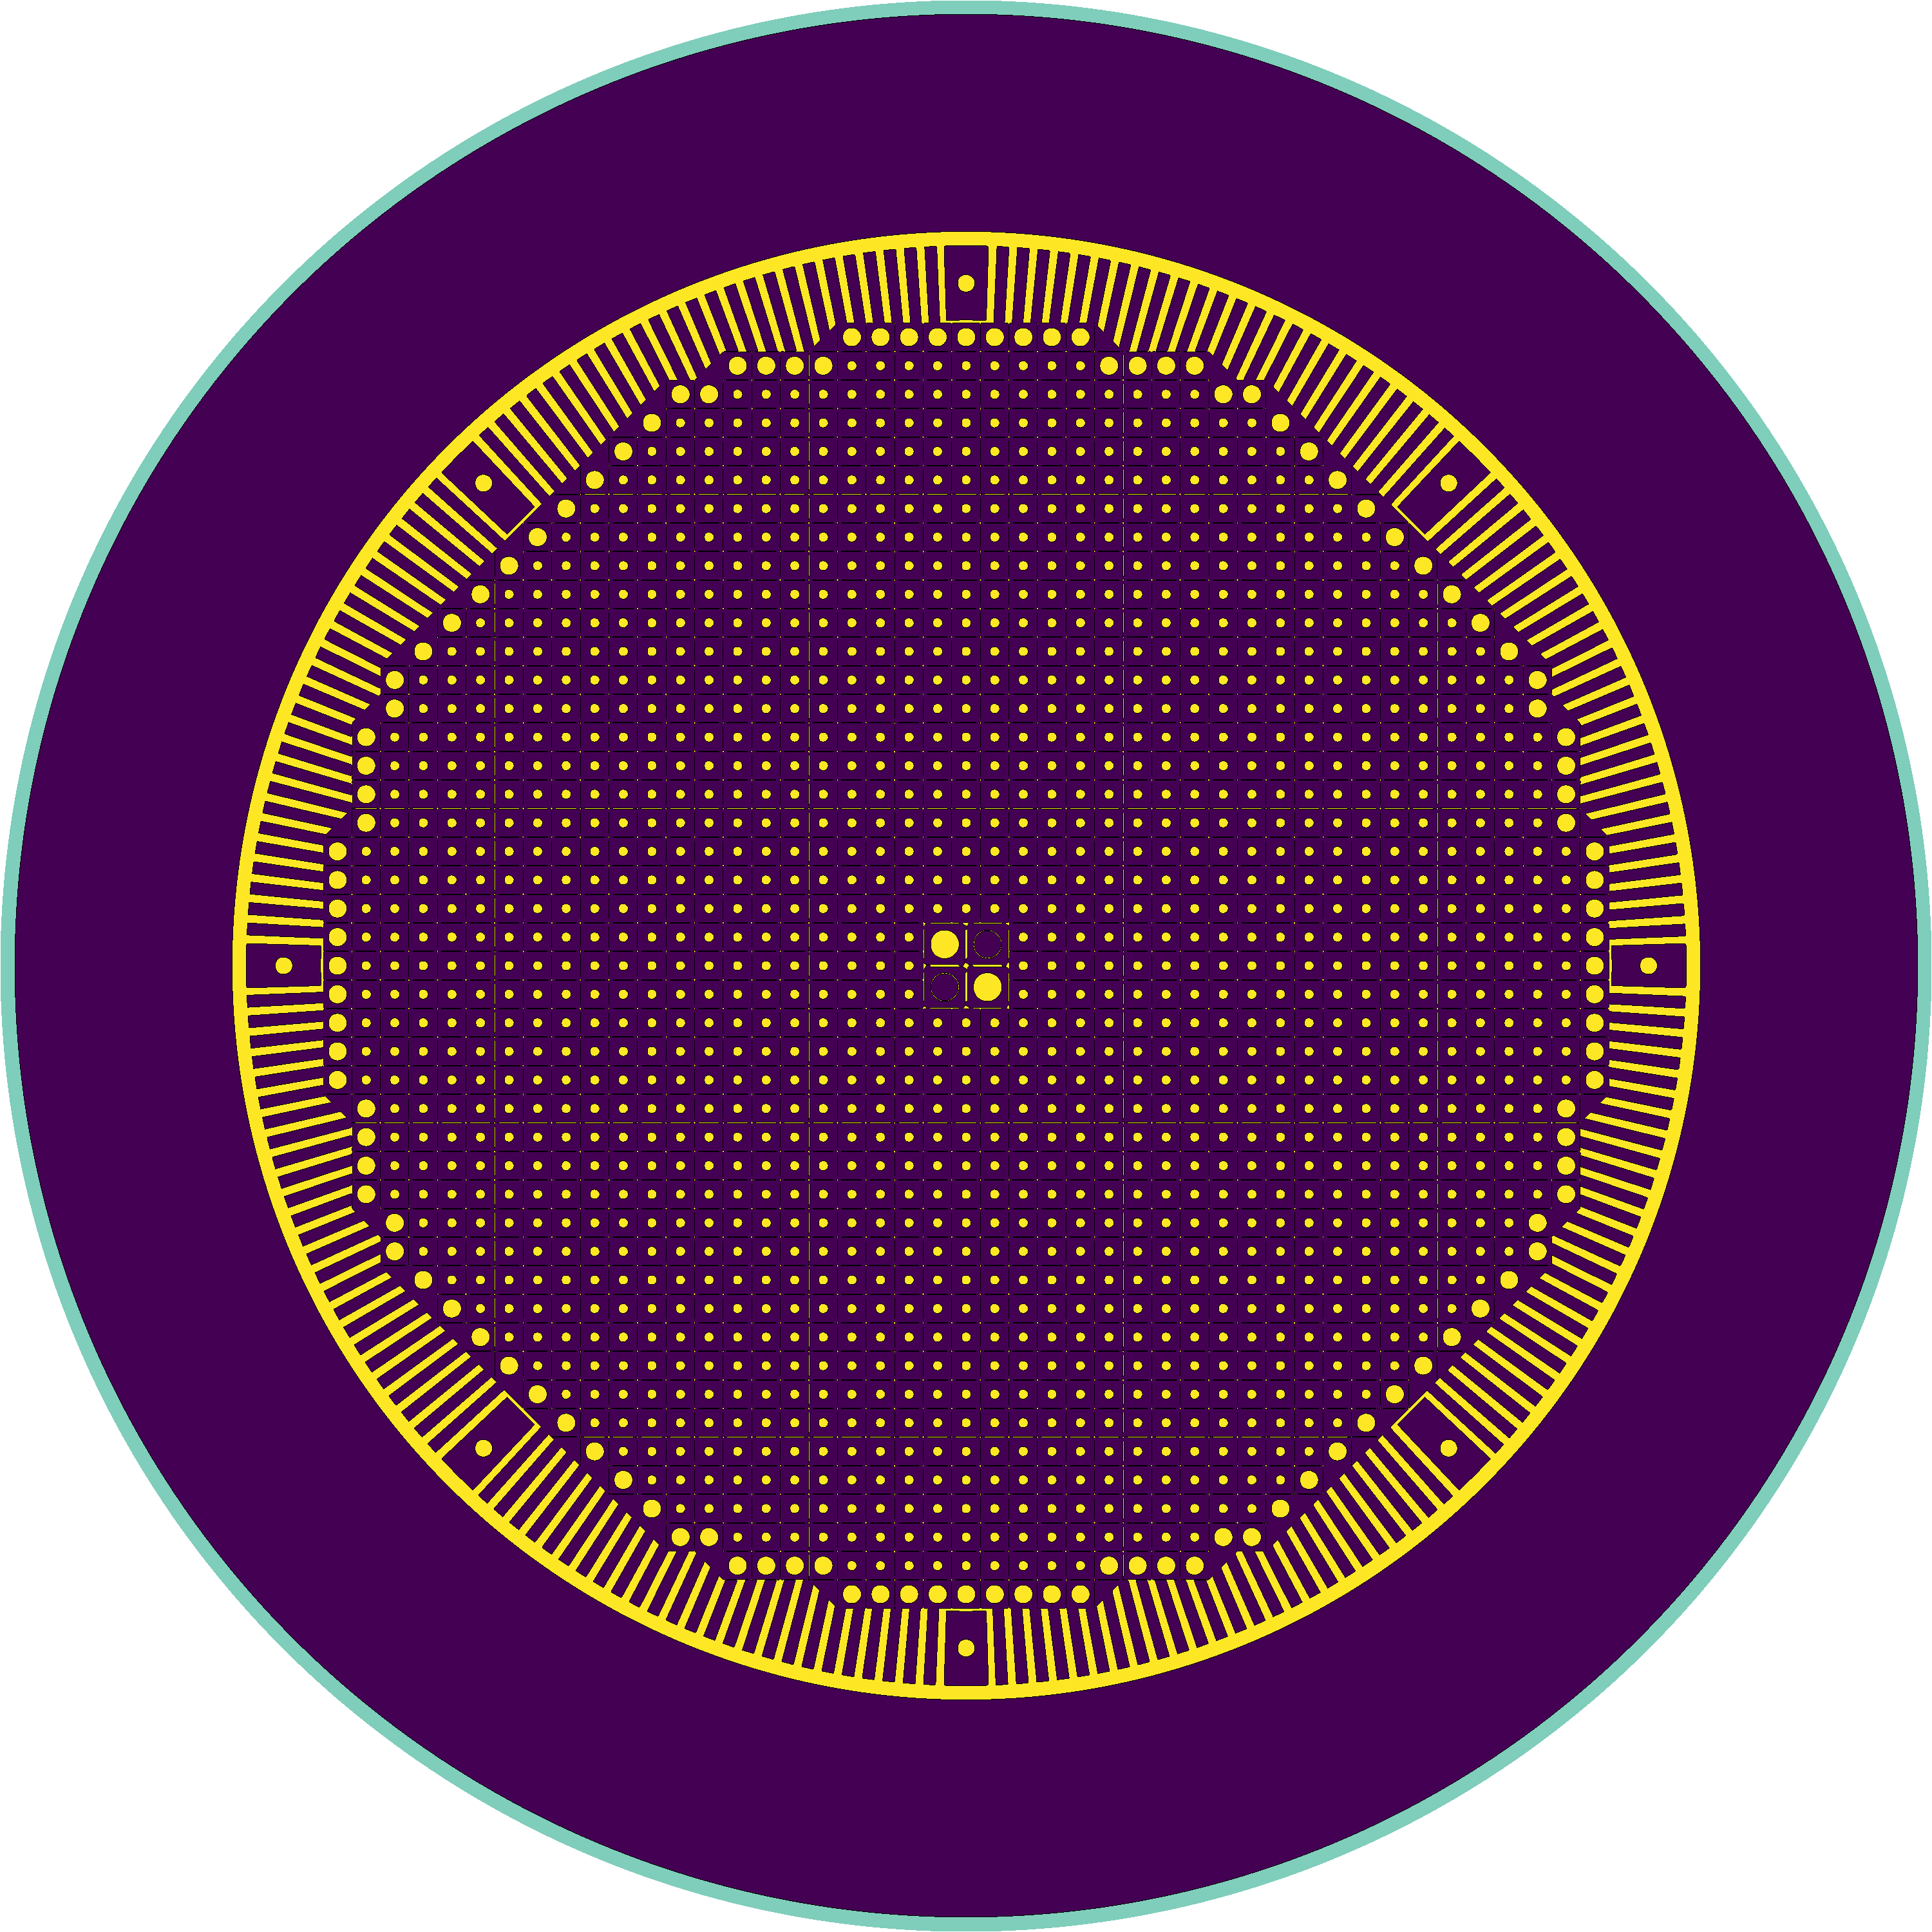
\includegraphics[width=\textwidth]{plan_view_ser.png}
  \caption{Plan view of SERPENT 2 \gls{MSBR} model developed in this work.}
  \vspace{-0.6em}
  \label{fig:serpent_plan_view}
\end{figure}
\FloatBarrier

\begin{figure}[hbp!] % replace 't' with 'b' to 
  \centering
  \vspace{-0.3em}
  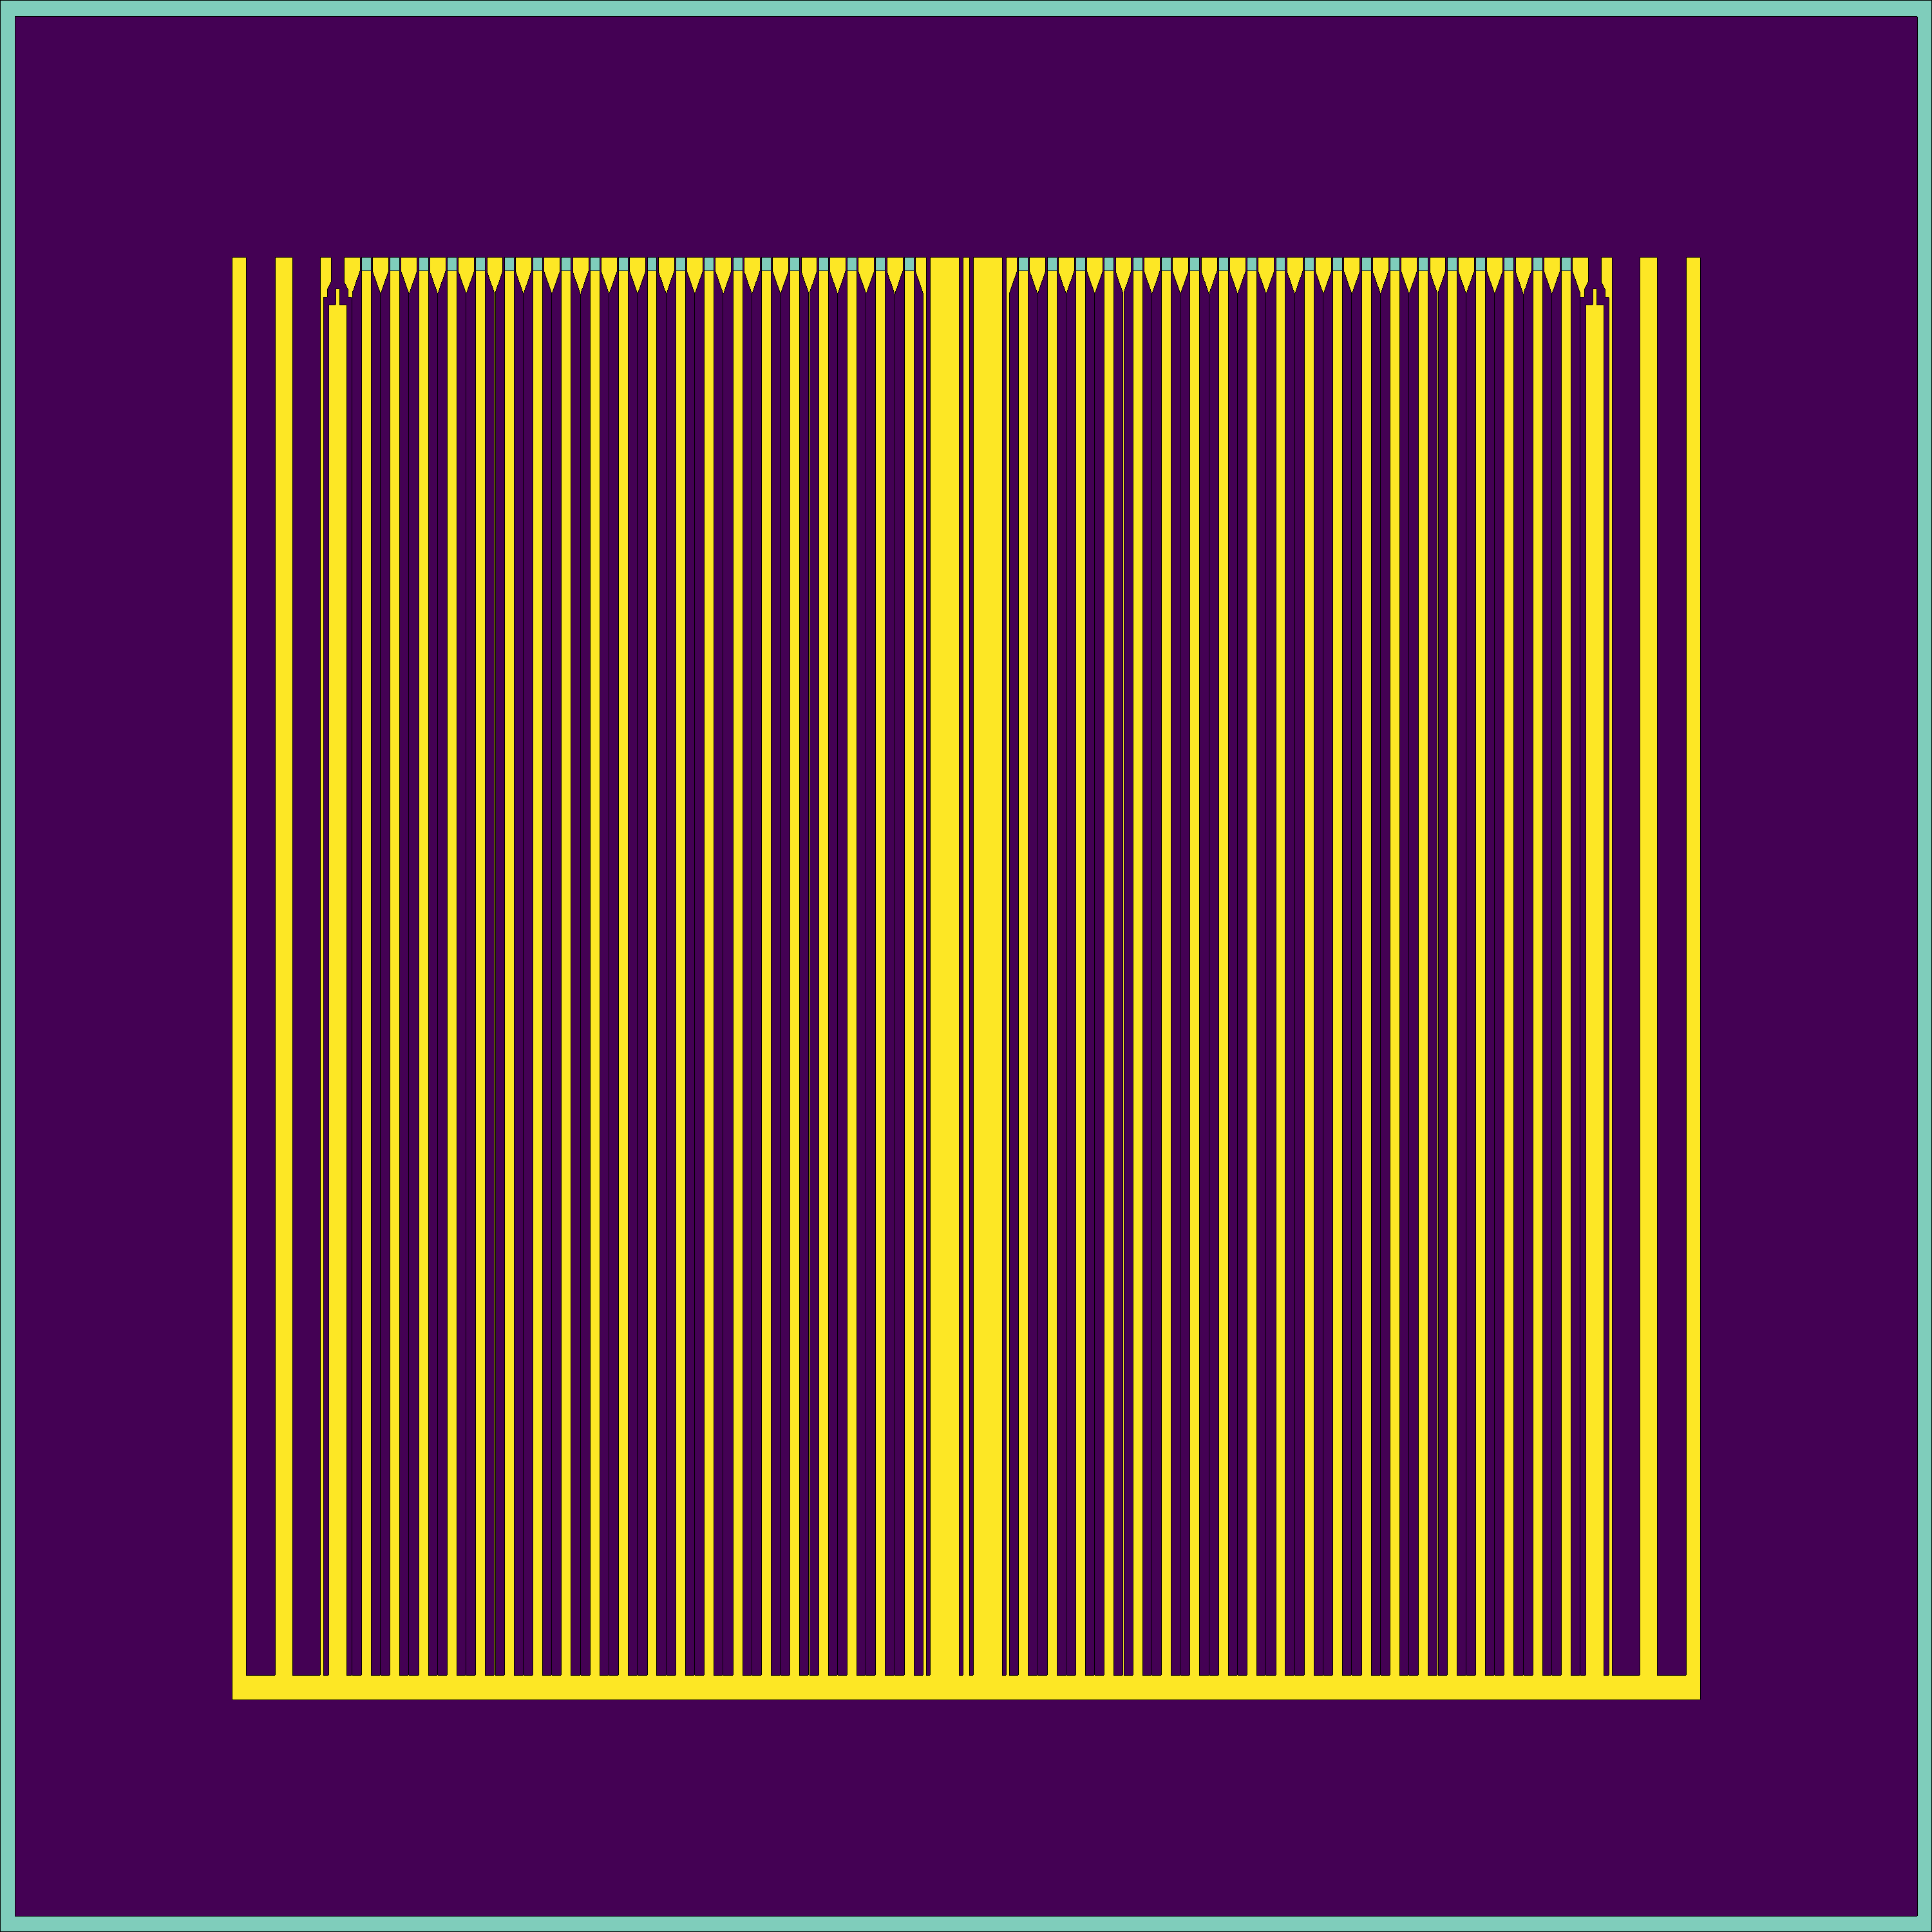
\includegraphics[width=\textwidth]{sect_view_ser.png}
  \caption{Elevation view of SERPENT 2 \gls{MSBR} model developed in this work.}
  \vspace{-0.6em}
  \label{fig:serpent_sectional_view}
\end{figure}
\FloatBarrier

In the model, zone I, zone II-A graphite blocks were described using circular cylinder and square cylinder surface types. The lengthwise ridges at each corner mentioned earlier were specified using dodecagonal cylindrical surfaces and general planes (figure~\ref{fig:I_element_ref}, \ref{fig:II_element_ref}). Zone I of the core was described using square lattices inscribed in the octagonal cylindrical surfaces to accurately represent geometry of that region.

The main challenge was to accurately represent zone II-B because it has irregular elements with sophisticated shapes. From the \gls{ORNL} report \cite{robertson_conceptual_1971}, the suggested design of zone II-B has 8 irregularly-shaped graphite elements every 45$^\circ$ as well as salt channels (figure~\ref{fig:detail_plan_view}). These graphite elements were simplified into right-circular cylindrical shapes  with central channels. Fig.~\ref{fig:serpent_zoneII} illustrates this core region in the SERPENT model. The volume of fuel salt in zone II was kept exactly 37\%, so that this simplification did not considerably change the core neutronics. This is the only simplification made to the \gls{MSBR} geometry in this work. 

\begin{figure}[hbp!] % replace 't' with 'b' to 
  \centering
  \vspace{-0.3em}
  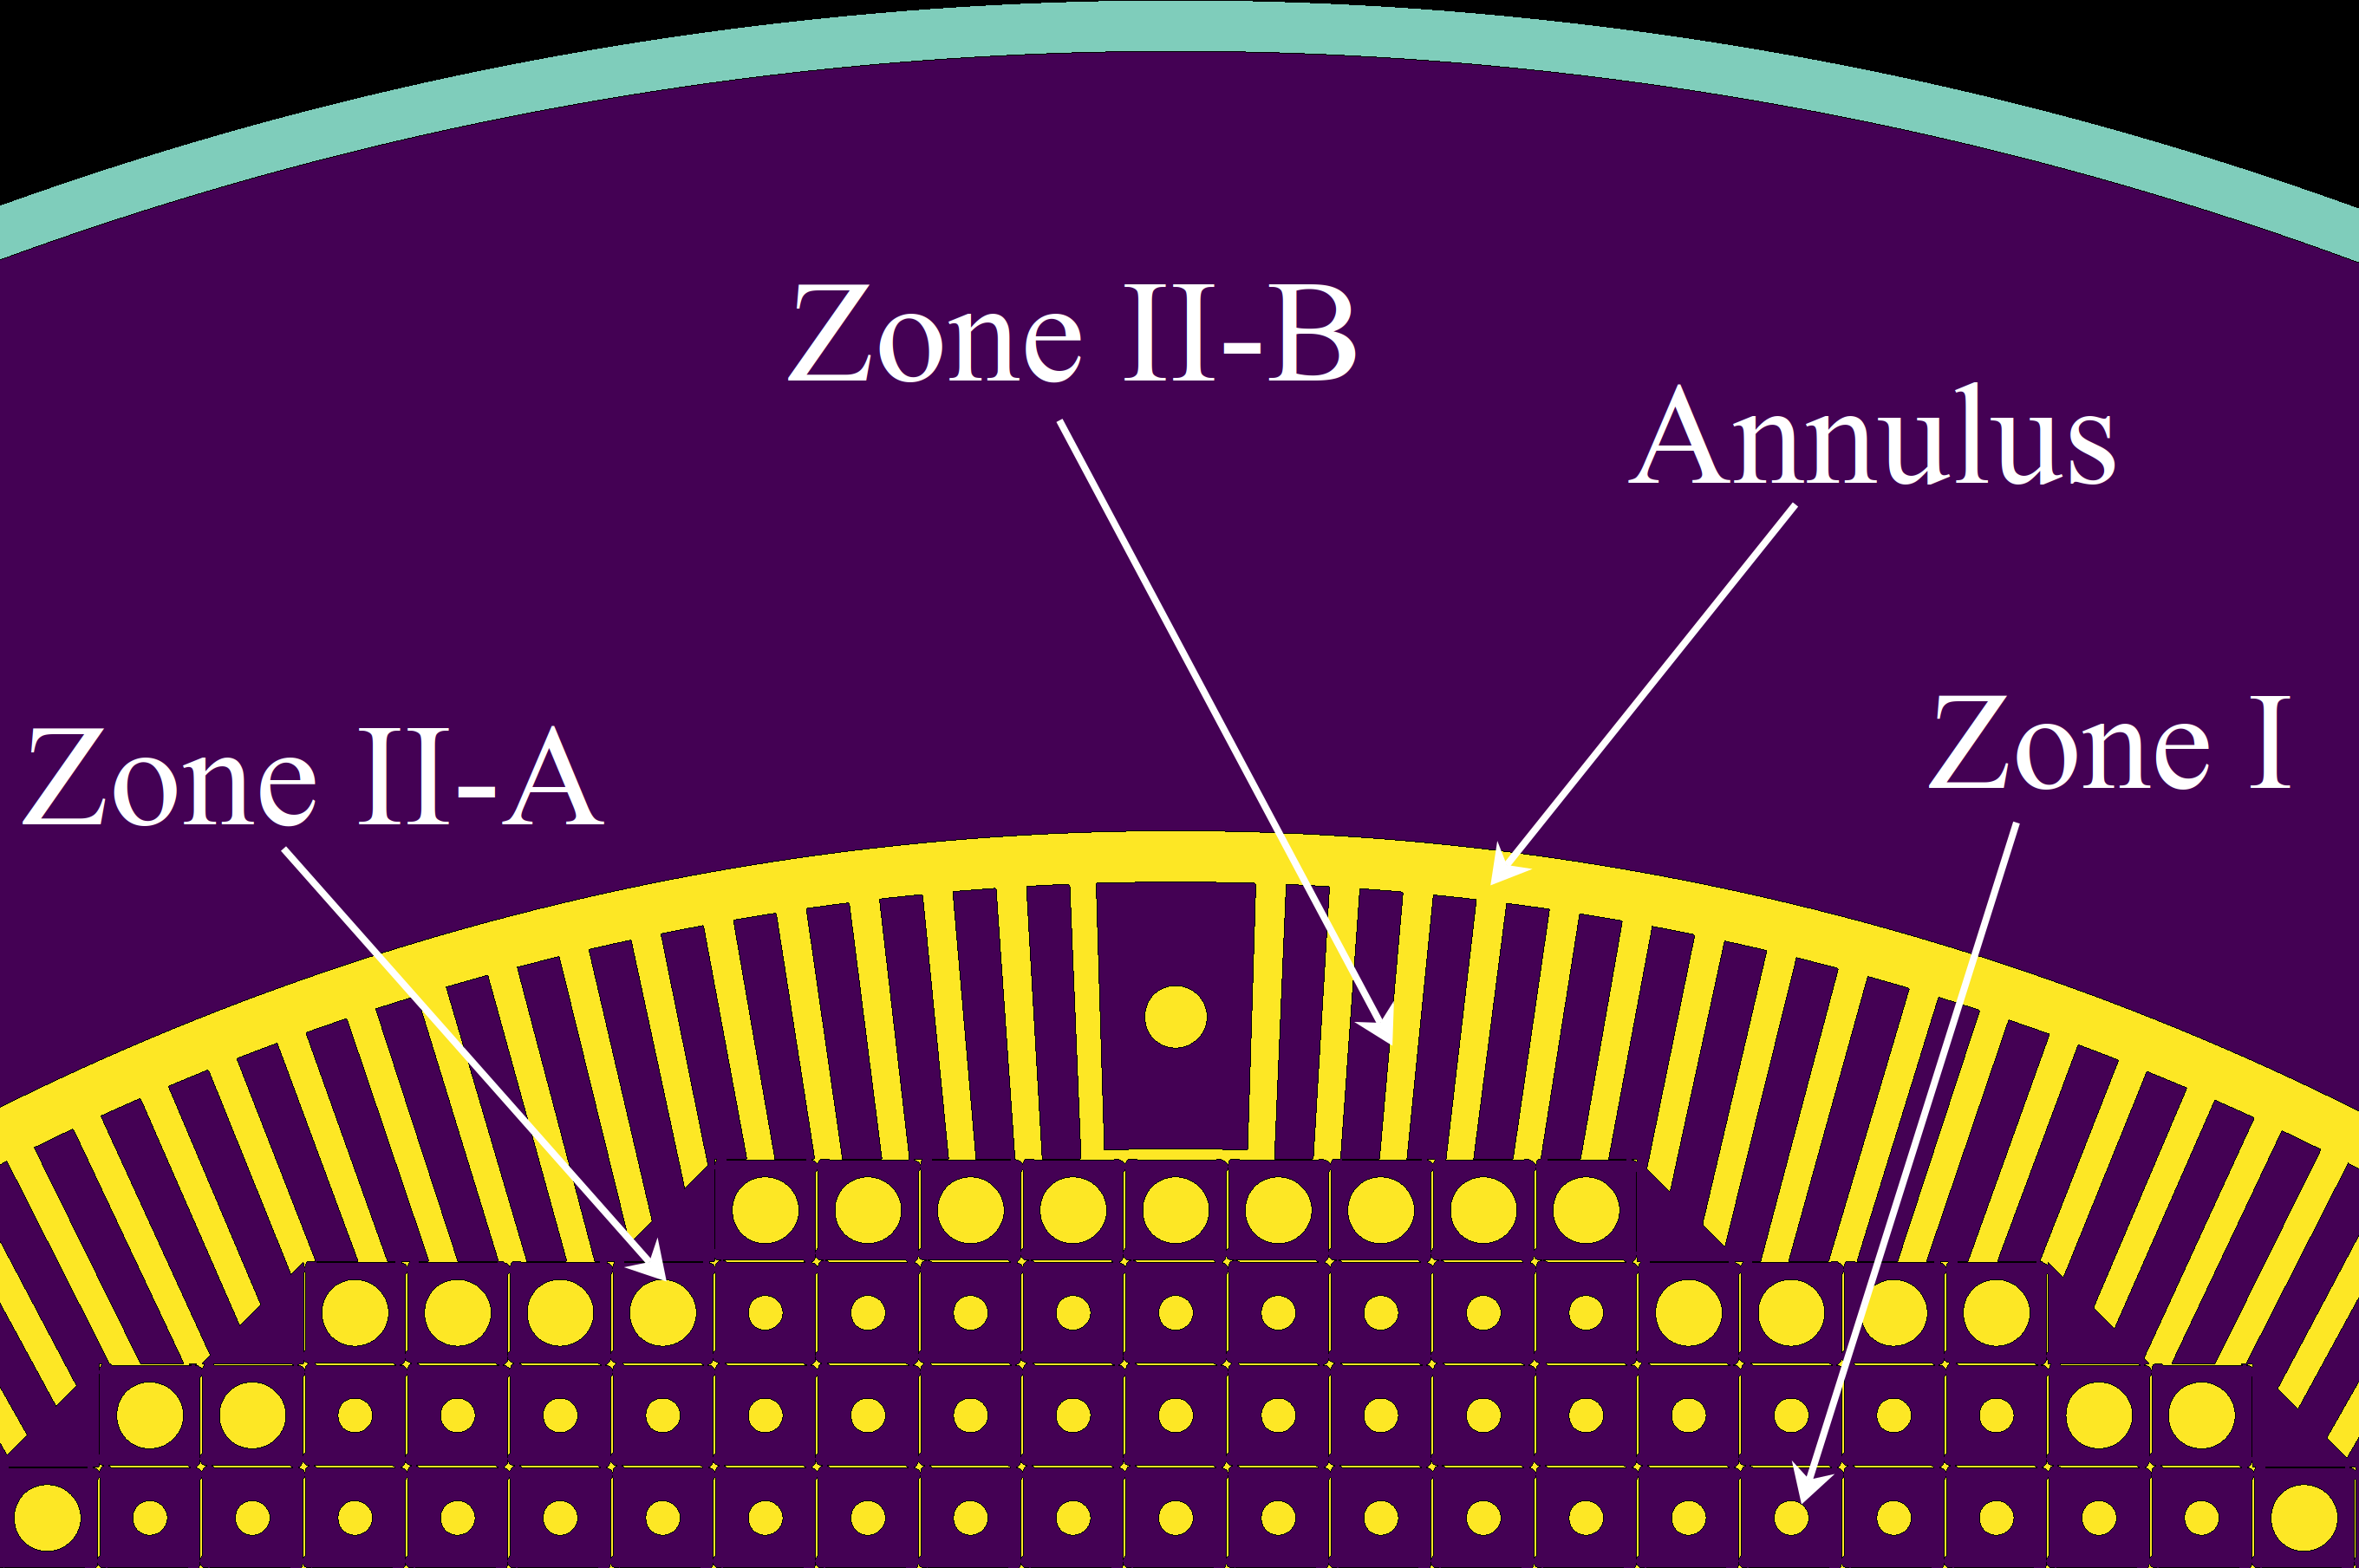
\includegraphics[width=\textwidth]{ser_zone_II.png}
  \caption{Detailed view of \gls{MSBR} zone II model.}
  \vspace{-0.6em}
  \label{fig:serpent_zoneII}
\end{figure}
\FloatBarrier

\subsection{Material composition and normalization parameters}
The fuel salt, the reactor graphite, and the modified Hastelloy-N\footnote{ Hastelloy-N is very common in reactors now but have been studied and developed at \gls{ORNL} in a program that started in 1950s.} are materials unique of the \gls{MSBR} and were created at \gls{ORNL}. The initial fuel salt used the same density (3.35 g/cm$^3$) and composition LiF-BeF$_2$-ThF$_4$-$^{233}$UF$_4$ (71.8-16-12-0.2 mole \%) as the \gls{MSBR} design\cite{robertson_conceptual_1971}. The lithium in the molten salt fuel is fully enriched in $^{7}$Li because $^{6}$Li is a very strong neutron poison and becomes tritium upon neutron capture. 

For cross section generation, JEFF-3.1.2 neutron library was employed \cite{oecd/nea_data_bank_jeff-3.1.2_2014}. The specific temperature was fixed for each material to correctly model the Doppler-broadening of resonance peaks when SERPENT generates the problem-dependent nuclear data library. The isotopic composition of each material at the initial state was described in detail in the MSBR conceptual design study \cite{robertson_conceptual_1971} and has been applied to SERPENT model without any modification. Table~\ref{tab:msbr_tab} is a summary of the major \gls{MSBR} parameters used by this model \cite{robertson_conceptual_1971}. 

%%%%%%%%%%%%%%%%%%%%%%%%%%%%%%%%%%%%%%%%
\begin{table}[h!]
        %\centering
        \caption{Summary of principal data for MSBR \cite{robertson_conceptual_1971}.}
        \begin{tabular}{|m{0.56\linewidth} | m{0.36\linewidth}|}
        \hline
        %\begin{tabularx}{\linewidth}{l X} \toprule 
                Thermal capacity of reactor           & 2250 MW(t)
                \\ [5pt] \hline 
                Net electrical output                 & 1000 MW(e) 
                \\ [5pt] \hline 
                Net thermal efficiency        & 44.4\%
                \\ [5pt] \hline 
                Salt volume fraction in central core zone     & 0.13
                \\ [5pt] \hline 
                Salt volume fraction in outer core zone       & 0.37
                \\ [5pt] \hline 
                Fuel salt inventory (Zone I)                  & 8.2 m$^3$	
                \\ [5pt] \hline 
                Fuel salt inventory (Zone II)                 & 10.8 m$^3$	
                \\ [5pt] \hline 
                Fuel salt inventory (annulus)                 & 3.8 m$^3$	
                \\ [5pt] \hline 
                Total fuel salt inventory                     & 48.7 m$^3$	
                \\ [5pt] \hline 
                Fissile mass in fuel salt                   & 1303.7 kg	
                \\ [5pt] \hline 
                Fuel salt components                  & 
                LiF-BeF$_2$-ThF$_4$-$^{233}$UF$_4$	
                \\ [5pt] \hline 
                Fuel salt composition                 & 
                71.85-16-12-0.25 mole\%
                \\[5pt]  \hline 
                Fuel salt density                    & 
                3.35 g/cm$^3$
                \\[5pt]  \hline 
        \end{tabular}
        \label{tab:msbr_tab}
\end{table}
%%%%%%%%%%%%%%%%%%%%%%%%%%%%%%%%%%%%%%%%%%%%%%%%


%\chapter[Online reprocessing simulation]{Online reprocessing simulation}

\section{Fuel salt processing systems}
Removing specific chemical elements from a molten salt is a complicated task that requires intelligent design (e.g., chemical separations equipment design, fuel salt flows to equipment) and has a considerable economic cost. This section contains \gls{MSBR} chemical processing plant and gas separation system brief overview.

\subsection{Fuel salt chemical processing facility}
All liquid-fueled \gls{MSR} designs involve varying levels of online fuel processing. Minimally, volatile gaseous fission products (e.g. Kr, Xe) escape from the fuel salt during routine reactor operation and must be captured. Additional systems might be used to enhance removal of those elements. Most designs also call for the removal of rare earth metals from the core since these metals act as neutron poisons. Some designs suggest a more complex list of elements to process (figure ~\ref{fig:periodic_tab}), including the temporary removal of protactinium from the salt or other regulation of the actinide inventory in the fuel salt \cite{ahmad_neutronics_2015}.

In the single-fluid \gls{MSBR} considered in this work, thorium, uranium, protactinium, and fission products are all mixed together in a single fluoride salt (FLiBe). Separation of thorium from lanthanide (atomic numbers 57 through 71) fission products is rather challenging because of their chemical similarities. 
\begin{figure}[htp!] % replace 't' with 'b' to 
  \centering
  \vspace{-0.3em}
  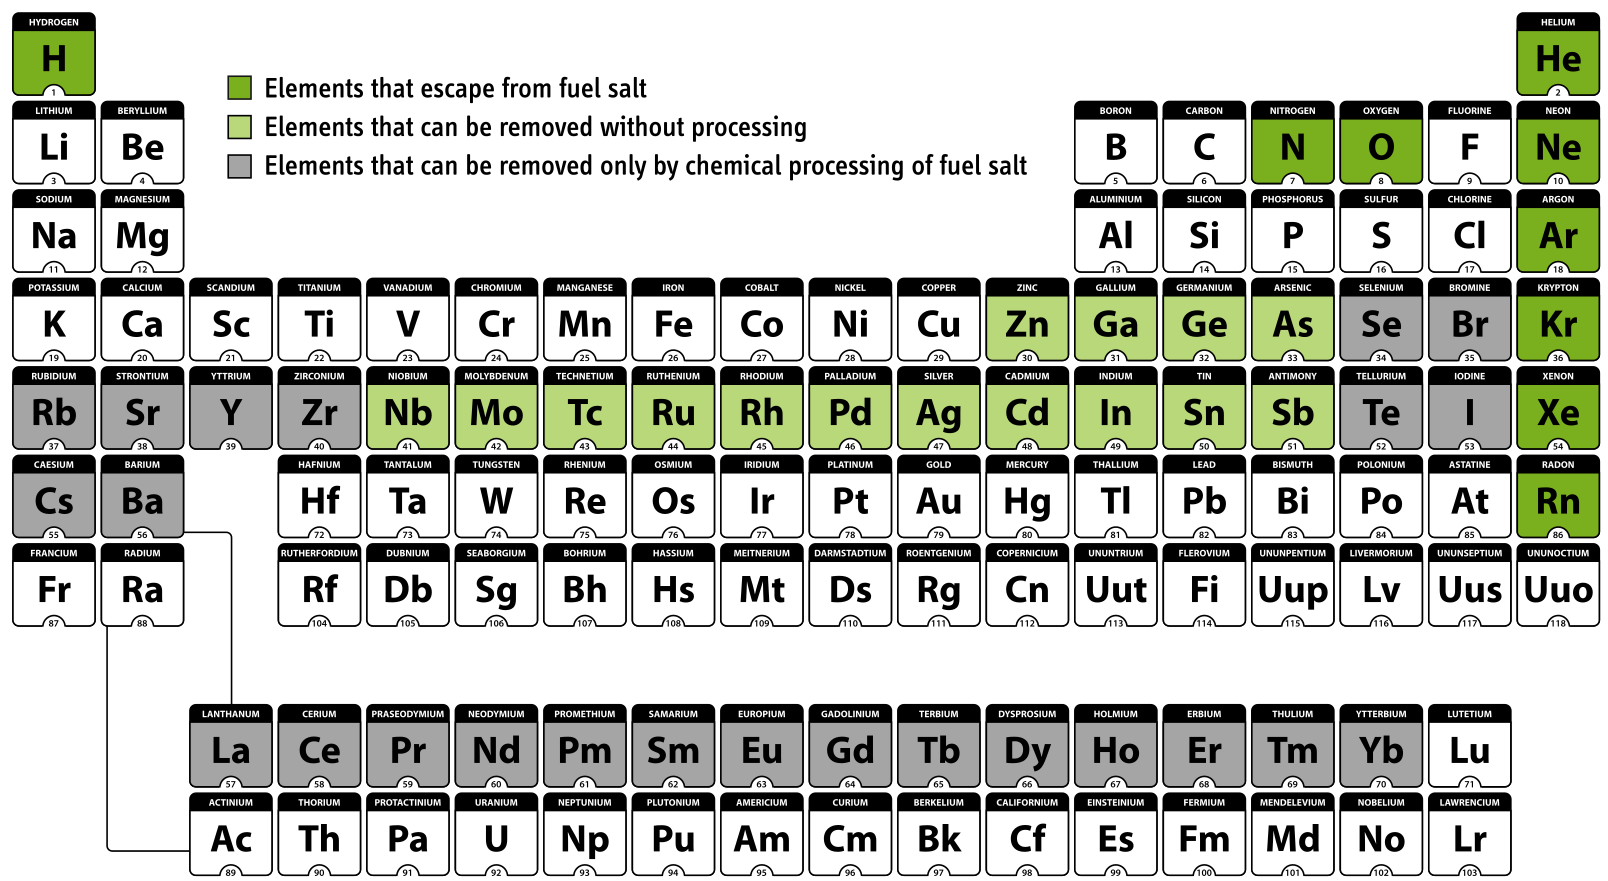
\includegraphics[width=\textwidth]{periodic_map.png}
  \caption{Processing options for \gls{MSR} fuels \cite{ahmad_neutronics_2015}.}
  \vspace{-0.6em}
  \label{fig:periodic_tab}
\end{figure}
\FloatBarrier

The principal scheme of \gls{MSBR} reprocessing facility concept is shown in Figure~\ref{fig:material_flow}. The fuel salt is first temporarily stored for cooling and decay of the shortest lived fission products, then directed to the primary fluorinator, where most of the uranium is removed by fluorination to UF$_6$. After that, the salt is routed to an extraction column where mixture containing metallic bismuth, lithium and thorium as reductants are contacted with the salt. The remaining uranium and protactinium are reductively extracted to the bismuth, leaving a salt that only contains fission products dissolved in carrier salt (base composition of LiF-BeF$_2$-ThF$_4$).The salt then goes through a reduction column where UF$_6$ is reduced to UF$_4$ in the salt, refueling it and preparing it for return to the reactor. Refill BeF$_2$ and ThF$_4$ are also added and all residual bismuth is removed from the salt. After a final cleanup step and valence adjustment, the purified salt returns to the reactor \cite{carter_design_1972,sorensen_one-fluid_2006}.

The bismuth accommodating some uranium and protactinium is routed to a hydrofluorination column where the metallic solutes in the bismuth are oxidized into their fluoride forms in the presence of a decay salt. The decay salt, containing UF$_4$, PaF$_4$, and ThF$_4$ passes into a decay tank where $^{233}$Pa is decaysto $^{233}$U. The uranium generated by protactinium decay is removed through fluorination to UF$_6$ and directed to the reduction column to refuel the purified fuel salt. A hydrofluorinator and a fluorinator can remove approximately \textbf{95\%} of the uranium from the stream.

The fully processed salt, on its way back to the reactor, has uranium added from the protactinium decay tank at the rate required to maintain or adjust the uranium concentration in the reactor (and, consequently, control the reactivity). This is performed by sparging the salt with UF$_6$ and hydrogen to produce UF$_4$ in the salt and HF gas \cite{robertson_conceptual_1971}.

\begin{figure}[htp!] % replace 't' with 'b' to 
  \centering
  \vspace{-0.3em}
  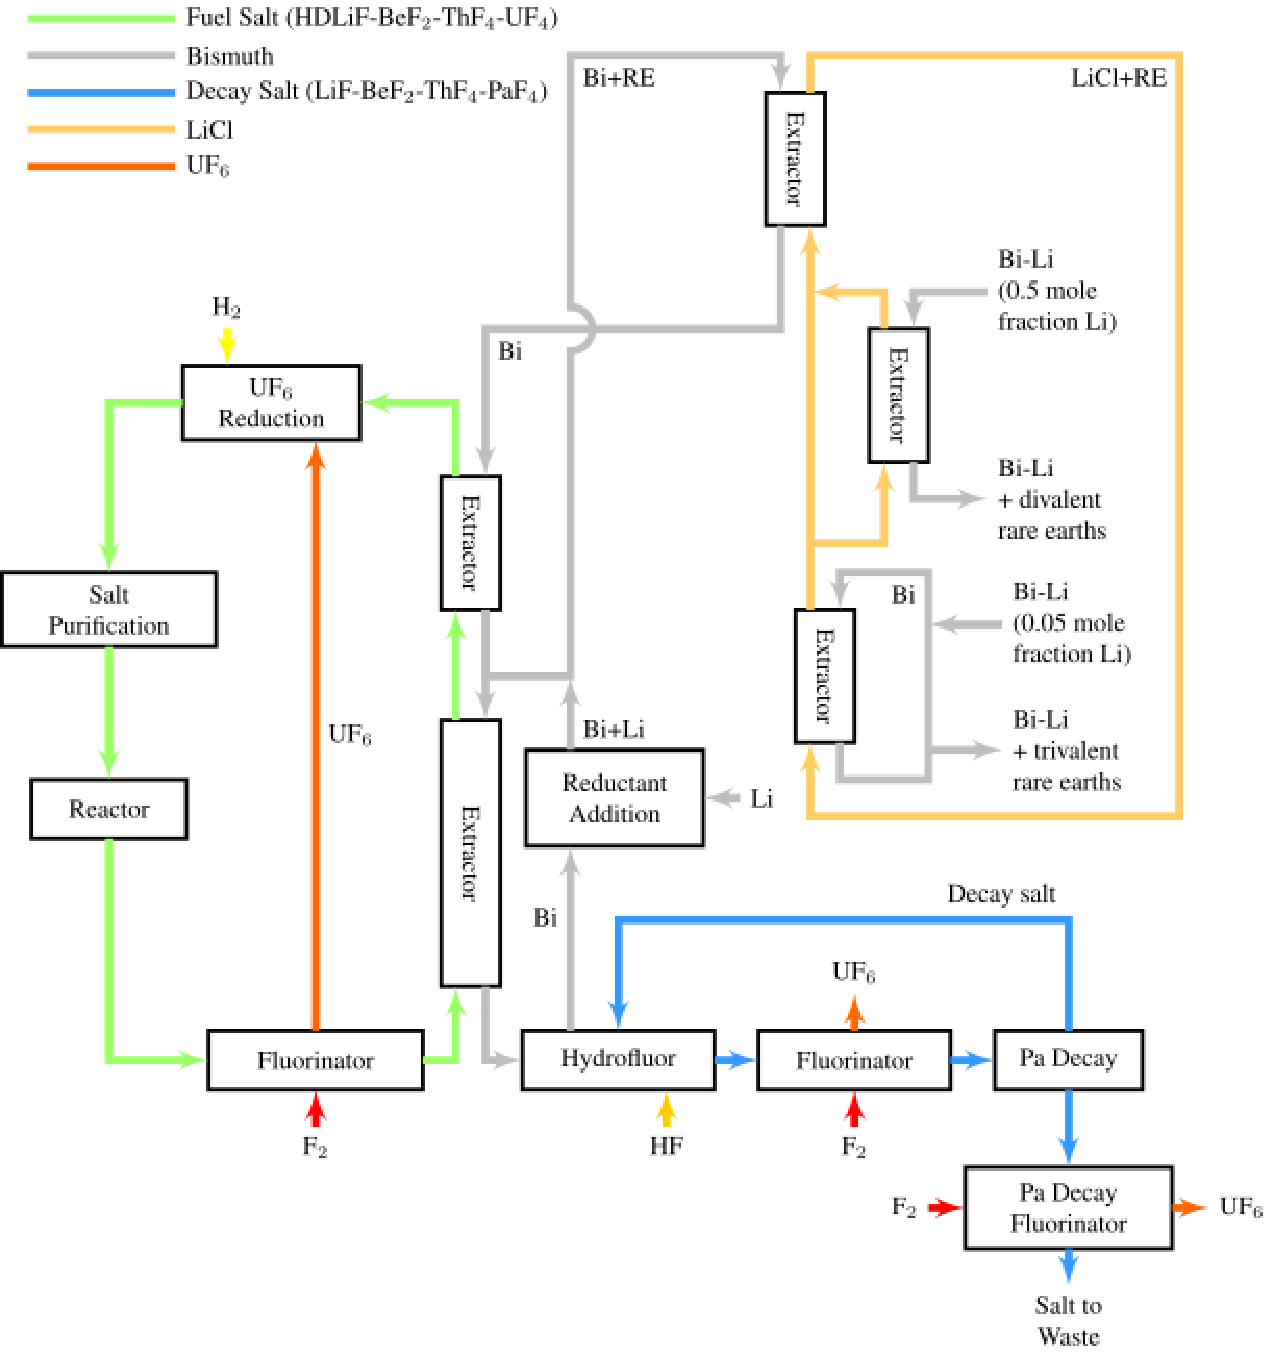
\includegraphics[width=\textwidth]{flowsheet.pdf}
  \caption{Detailed block diagram of chemical processing scheme for single-fluid \gls{MSBR} \cite{robertson_conceptual_1971, sorensen_one-fluid_2006}.}
  \vspace{-0.6em}
  \label{fig:material_flow}
\end{figure}
\FloatBarrier

\subsection{Gas separation system}
Volatile gaseous fission products (e.g. Kr, Xe) must be removed from the fuel salt to avoid reactor poisoning especially during starup and power maneuvering. This is particularly true for $^{135}$Xe, with its very large absorption cross section. Tritium, xenon, and krypton are sparged from the fuel salt by helium introduced in a bypass stream by a bubble generator and subsequently removed by a gas separator. Indeed, noble gases, because of their exceptional insolubility in the salt, will migrate promptly to any gaseous interface available. Because they form ideal-dilute mixture in salt (obey Henry's law), they will migrate in accordance with the conventional laws of mass transfer. If tiny helium bubbles are circulated with the fuel salt, they will absorb xenon and krypton fission products. The fission-product-rich bubbles of helium may then be separated from the salt and discharged to the off-gas system. Xenon migration to the circulating bubbles is in competition with xenon migration to the porous moderator graphite. The graphite is especially of concern because it absorbs xenon and holds it in the core which leads to parasitic neutron absorption. The 0.5\% target value for $^{135}$Xe poison fraction can be achieved when circulating helium bubbles 0.508mm in diameter \cite{robertson_conceptual_1971}. This is accomplished by bypassing 10\% of the fuel salt from the pump discharge through a bubble separator to remove the xenon bubbles and then back into the pump suction, as shown in Figure~\ref{fig:gas_removal_system}. The average residence time of a bubble in the fuel loop would be 10 full cycles.

\begin{figure}[htp!] % replace 't' with 'b' to 
  \centering
  \vspace{-0.3em}
  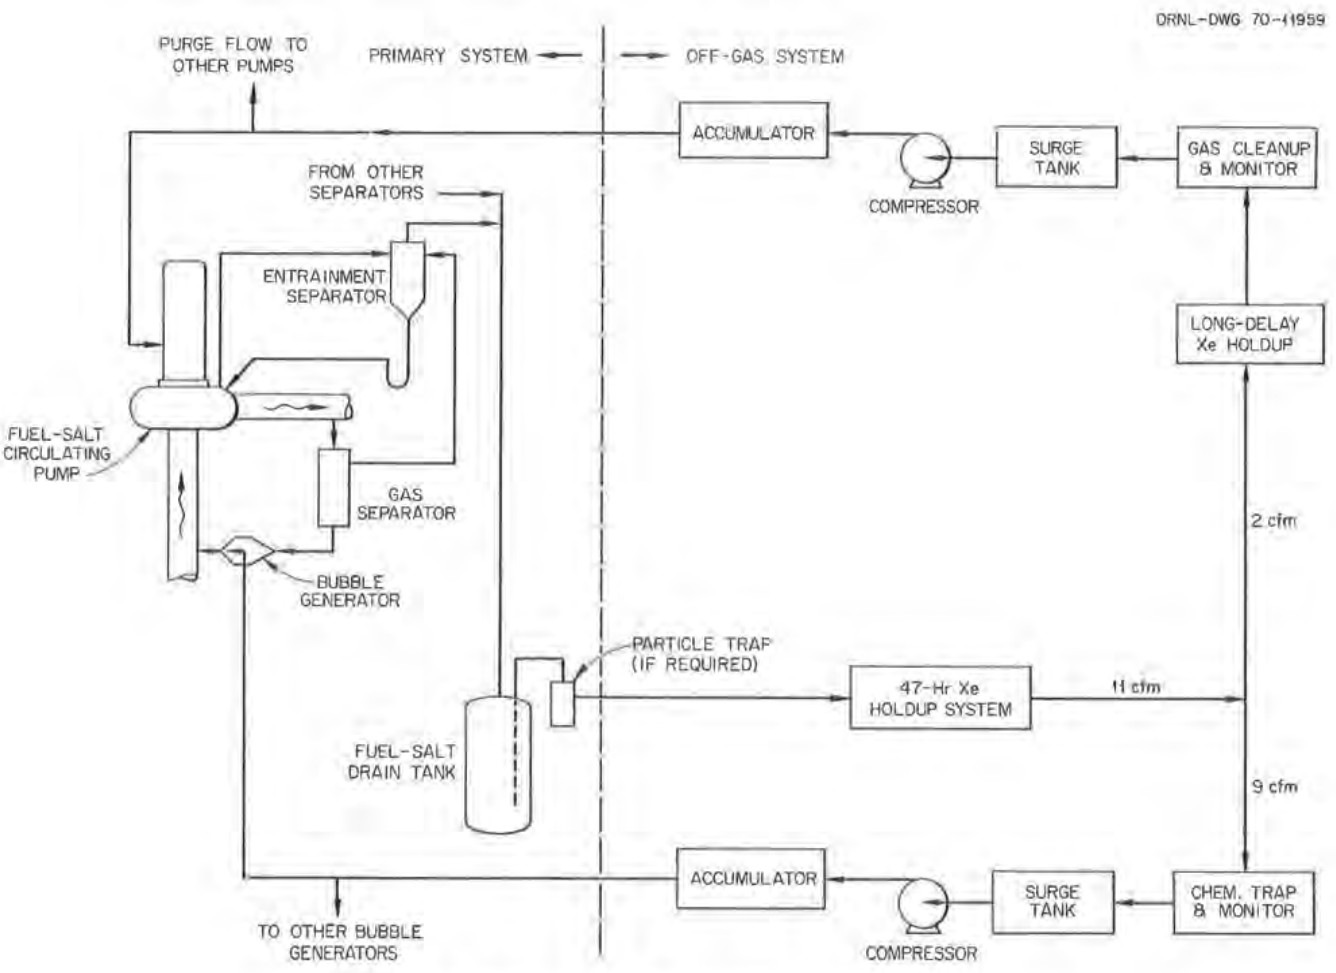
\includegraphics[width=\textwidth]{gas_separation.png}
  \caption{Flow diagram for \gls{MSBR} plant. Green line indicates gas separation and off-gas system \cite{robertson_conceptual_1971}.}
  \vspace{-0.6em}
  \label{fig:gas_removal_system}
\end{figure}
\FloatBarrier
\section{Online reprocessing method}
Modeling liquid-fueled systems with existing neutron transport and depletion tools is challenging because most of these tools are designed for the solid-fueled reactors simulation. The fuel material flows and potential online separations or feeds of specific elements or nuclides are the main challenges of liquid-fueled systems. SaltProc accounts for online feeds and separations using SERPENT 2 neutron transport and burnup capabilities.

\subsection{Online separations and feeds}
The ability to perform online fuel salt reprocessing improves the potential neutronic performance of liquied-fueled reactors. Firstly, it is unnecessary for liquid-fueled reactors to operate with excess reactivity because fissile material is continuously being added into the core. Secondly, continuously removing fission products including strong absorbers (poisons) should significantly improve fuel utilization and decrease parasitic neutron absorption. Finally, neutronic parameters could be adjusted ``on-the-fly" without operational cycle interruption. Nevertheless, removal of each element from the liquid fuel salt presents a unique challenge in terms of storage and disposal of the separated materials.

To take into account online reprocessing, two potential approaches can be implemented. One is a batch-wise approach where material is moved into or from the core at specific time intervals (batch). This approach assumes that material accumulation in the core during the time between separations or feeds does not affect reactor physics. This method requires the simulation to stop, modify the fuel composition, and restart. This approach was implemented in a ChemTriton script \cite{powers_new_2013} which has been developed by T.J.Harrision, \gls{ORNL}, and actively using for online reprocessing simulation with SCALE/TRITON \cite{bowman_scale_2011} and Shift \cite{pandya_implementation_2016}. 

Another approach approximates more continuous reprocessing where material is separated from (or added into) the core at all times to simulate true continuous online reprocessing. This method is more difficult because it requires adding a term to the Bateman equations. In SCALE/TRITON, ORIGEN \cite{gauld_isotopic_2011} solves a set of Bateman equations using one-group averaged fluxes and cross-sections obtained from a transport calculation. Bateman equations that describe the rate of change of the isotopes due to neutron induced reactions and decay
processes could be written in this form \cite{aufiero_extended_2013}:

\begin{align}
        \frac{dN_i}{dt} &= \bar{\Phi}\sum\limits_{j}N_{j}\sigma_{j \rightarrow 		i} - \bar{\Phi}\sum\limits_{j}N_{i}\sigma_{i \rightarrow j} + \sum					\limits_{j}	N_{j}\lambda_{j}b_{j \rightarrow i} - N_{i}\lambda_{i}
\label{eq:bateman}
	\intertext{where} 
	N_i &= \mbox{number density of isotope i} \\
	N_j &= \mbox{number density of isotope j} \\
	\bar{\Phi} &= \mbox {average in the space and energy neutron flux} \\
	\sigma_{j \rightarrow i} &= \mbox{microscopic one-group transmutation cross section} \\
	\lambda_i &= \mbox{decay constant of nuclide i} \\
	\lambda_j &= \mbox{decay constant of nuclide j} \\
	b_{j \to i} &= \mbox{branching fractions of radioactive decay from nuclide j}
\end{align}

The four terms on the right-hand side of the equation represent (1) the production rate of nuclide $i$ from irradiation, (2) the loss rate of nuclide $i$ due to irradiation, (3) the decay rate of nuclide $j$ into nuclide $i$, and (4) the loss rate of nuclide $i$ due to decay. Mentioned earlier deterministic codes SCALE/TRITON and Monte Carlo codes MCNP, Shift, KENO-VI do not support non-zero removal or feeds rates for depletion simulations.

Online fuel reprocessing can be explicitly introduced in the system of equations by adding effective decay and transmutation terms for the various nuclides. During fuel composition evolution calculations, the total mass fraction of thorium fluoride is kept constant at 12\%. For this purpose, $^{233}$Th isotope is replaced with the fresh $^{232}$Th feed material. This could be achieved with an additional gain term on the right-hand side of the Bateman equation:
\begin{align*}
\bar{\Phi}\sum\limits_{k=^{232}Th}N_{k}\sigma_{k,c}
\end{align*}
where $\sigma_{k,c}$ is the one-group capture cross section of thorium-232.

The removal of fission products and protactinium is achieved by adding an explicit decay term to the Bateman equations. For the generic fission product, l, loss term can be added:
\begin{align*}
- N_{l}\lambda_{l,reproc}
\end{align*}
where $\lambda_{l,reproc}$ is the effective removal time constant of the particular chemical species. This approach was recently implemented as a purpose-made extension within the continuous-energy Monte Carlo reactor physics and burn-up code SERPENT \cite{aufiero_extended_2013} but it is not currently available for external users.

I have developed the SaltProc Python package \cite{andrei_rykhlevskii_arfc/saltproc:_2018}, implementing batch-wise approach coupled with the SERPENT 2 burnup routine. A high-fidelity full-core \gls{MSBR} model serves as a basis for the online reprocessing simulation described in this thesis. 

\subsection{Fuel material flows}
The $^{232}$Th in the fuel absorbs thermal neutrons and produces $^{233}$Pa which then decays into the fissile $^{233}$U. Furthermore, the \gls{MSBR} design requires online reprocessing to remove all poisons (e.g. $^{135}$Xe), noble metals, and gases (e.g. $^{75}$Se, $^{85}$Kr) every 20 seconds. Protactinium presents a challenge, since it has a large absorption cross section in the thermal energy spectrum. Accordingly, $^{233}$Pa is continuously removed from the fuel salt into a protactinium decay tank to allow $^{233}$Pa to decay to $^{233}$U without poisoning the reactor. The reactor reprocessing system is designed to separate $^{233}$Pa from the molten-salt fuel over 3 days, hold it while $^{233}$Pa decays into $^{233}$U, and return it back to the primary loop. This feature allows the reactor to avoid neutron losses to protactinium, keeps fission products to a very low level, and increases the efficiency of $^{233}$U breeding. Table~\ref{tab:reprocessing_list} summarizes full list of nuclides and the cycle times used for modeling salt treatment and separations \cite{robertson_conceptual_1971}. 

%%%%%%%%%%%%%%%%%%%%%%%%%%%%%%%%%%%%%%%%
\begin{table}[ht!]
        \centering
        \caption{The effective cycle times for protactinium and fission products removal (reproduced from \cite{robertson_conceptual_1971}).}
        \begin{tabular}{|m{0.25\textwidth} | m{0.45\textwidth}|m{0.16\textwidth}|}
        \hline 
        %\begin{tabularx}{\linewidth}{l X} \toprule 
        Processing group & \qquad\qquad\qquad Nuclides & Cycle time (at full power) \\ [5pt] \hline 
        Rare earths & Y, La, Ce, Pr, Nd, Pm, Sm, Gd & 50 days \\ [5pt] \hline 
        \qquad & Eu & 500 days \\ [5pt] \hline
        Noble metals & Se, Nb, Mo, Tc, Ru, Rh, Pd, Ag, Sb, Te & 20 sec \\ [5pt] \hline
        Seminoble metals & Zr, Cd, In, Sn & 200 days \\ [5pt] \hline
        Gases & Kr, Xe & 20 sec \\ [5pt] \hline
        Volatile fluorides & Br, I & 60 days \\ [5pt] \hline
        Discard & Rb, Sr, Cs, Ba & 3435 days \\ [5pt] \hline
        Salt discard & Th, Li, Be, F & 3435 days \\ [5pt] \hline
        Protactinium & $^{233}$Pa & 3 days \\ [5pt] \hline
        Higher nuclides & $^{237}$Np, $^{242}$Pu & 16 years \\ [5pt] \hline
        \end{tabular}
        %\footnotetext{Chemical processing plant and gas separation system removing chemical elements (not isotopes) only. Isotopes instead of elements listed because other isotopes are short-lived and might be ignored.}
        \label{tab:reprocessing_list}
          \vspace{-0.9em}
\end{table}
Since removal rates vary among nuclides in this reactor concept, the built-in SERPENT 2 reprocessing subroutine is unable to capture the desired reprocessing strategy. The removal rates also dictate the necessary resolution of depletion calculations. If the depletion time intervals are very short, an enormous number of depletion steps are required to obtain the equilibrium composition. On the other hand, if the depletion  calculation time interval is too long, the impact of short-lived fission products is not captured. To compromise, the time interval for depletion calculations in this model was selected as 3 days to correlate with the removal interval of $^{233}$Pa and $^{232}$Th was continuously added to maintain the initial mass fraction of $^{232}$Th.

\subsection{Simplifying assumptions}
The main goal of the present study is to identify the effects adjusting the fuel salt composition, and find equilibrium performance of a thorium \gls{MSBR} fuel cycle. To highlight these effects and simplify the analysis, several assumptions have been made.

First of all, thorium loading during operation was held constant and equal to initial thorium loading (i.e. $m_{Th}(t)=m_{Th}(0)$) with a variable feed rate (in kg/day) of fresh thorium. Because thorium is a fertile material with relatively high absorption cross section, this has important impacts on reactor physics, including negatively impacting reactivity and skewing the fuel-to-moderator ratio which makes neutron energy spectrum harder. While a reduction in the thorium loading reduces the amount of initial fissile material required to achieve criticality, the breeding rate of $^{233}$U should be sufficient to maintain the core critical during operation.

The solubility of heavy metals is a known problem for \glspl{MSR} but it is fundamentally dependent on the type of carrier salt. For this work, solubility limits for uranium were neglected because the molar fraction of UF$_4$ was negligible for the accuracy desired in this work. In addition, this work assumed that addition or removal of soluble material (e.g. UF$_4$) has a small influence on the fuel salt volume, this volume change is not treated here.

Figure~\ref{fig:th_cycle} from Chapter 2 demonstrates that transformation from $^{232}$Th to $^{233}$U is slow process because $^{233}$Pa $\beta$-decay has half-life 27.4 days. Thus, approximately 90 days needed to decay 90\% of $^{233}$Pa to $^{233}$U. Figure~\ref{fig:pa_isolation} shows how protactinium is separated from the fuel salt reprocessing flow. Therefore, if protactinium decay tank is empty at the moment of reactor startup, then the expected fissile material stream would appear only after a few months of reactor operation at full power. To avoid time-dependent feed rate for $^{233}$UF$_4$ it is assumed that the protactinium decay tank initially contain some amount of $^{233}$UF$_4$, and the rate of fissile material flow from the tank to the core is set equal to the $^{233}$Pa removal rate. Moreover, simulated cycle time at full power was set to 20 years ($\approx$ 7300 days). Finally, 100\% reprocessing separation efficiency was assumed.

\begin{figure}[hbp!] % replace 't' with 'b' to 
  \centering
  \vspace{-0.3em}
  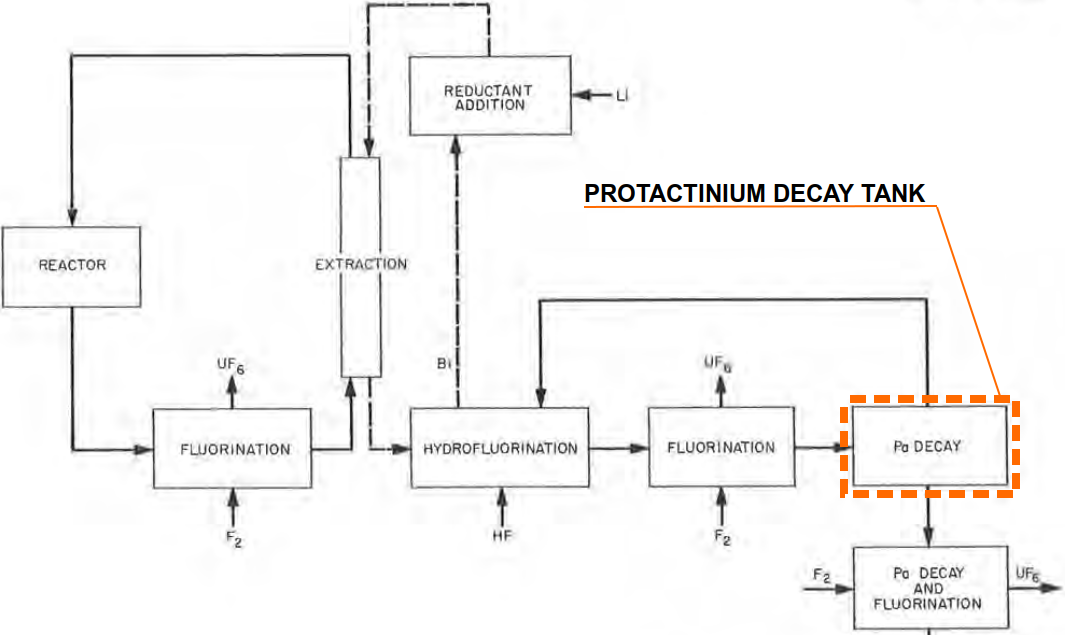
\includegraphics[width=\textwidth]{pa_isolation.png}
  \caption{Protactinium isolation with uranium removal by fluorination \cite{robertson_conceptual_1971}.}
  \vspace{-1.6em}
  \label{fig:pa_isolation}
\end{figure}
\FloatBarrier

The thermal fission of a $^{233}$U in fluoride salts oxidizes the salt. This happens because the uranium nucleus balances the charge of four fluorine ions in the salt (e.g. $^{233}$UF$_4$), but fission products tend to not bind to all the four fluorines released after the uranium fissions. Figure~\ref{fig:excess_fluorine} demonstates an example of an oxidative fission reaction. This excess of fluorine must be compensated, otherwise chemical reactions harmful to reactor components would occur \cite{ridley_method_2017}. In this study, fission-driven salt oxidation is ignored.

\begin{figure}[htp!] % replace 't' with 'b' to 
  \centering
  \vspace{-0.3em}
  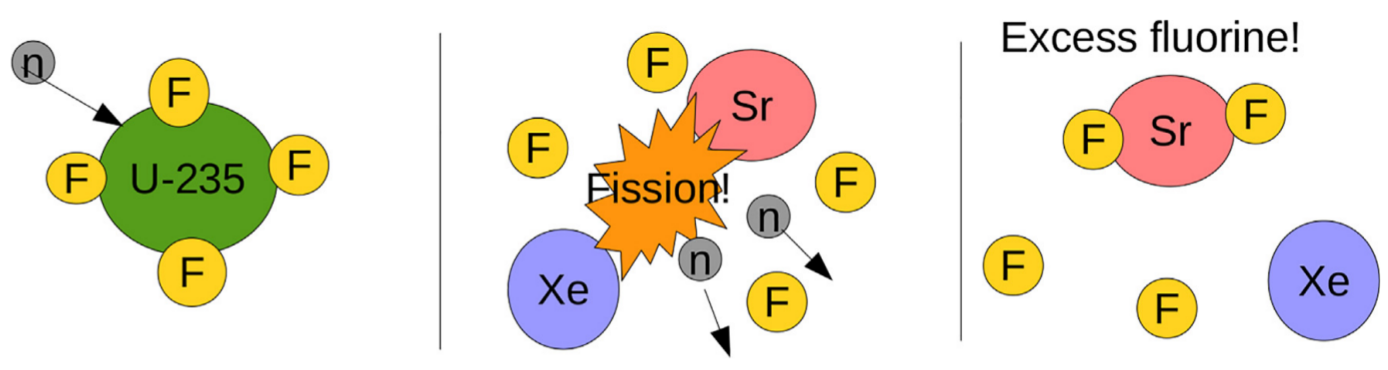
\includegraphics[width=0.8\textwidth]{excess_fluorine.png}
  \caption{Process of production an excess of fluorine due to fission of a $^{233}$U in fluoride salts \cite{ridley_method_2017}.}
  \vspace{-1.0em}
  \label{fig:excess_fluorine}
\end{figure}
\FloatBarrier

Finally, for this study, equilibrium is defined as when $k_{eff}$ and the $^{233}$U concentration in the fuel salt vary less than one percent over several months. 

\section{Python code description}
The objectives for the SaltProc tool were to expand SERPENT 2 burn-up capabilities for modeling liquid-fueled \gls{MSR} and provide an open-source tool for the simulation of reactors where material is removed or added at any time during fuel irradiation. The Python 2.7 packages uses HDF5 \cite{the_hdf_group_hierarchical_1997} to store data and the Nuclear Engineering Toolkit - PyNE \cite{scopatz_pyne:_2012} for SERPENT output file parsing. As was discussed earlier, SaltProc maintains the iterative semi-continuous approach to simulate continuous feeds and removals.

The tool structure and capabilities are similar to ChemTriton tool for SCALE developed in \gls{ORNL} \cite{powers_new_2013}. SaltProc is coupled with Monte Carlo SERPENT 2 software which allows to simulate online reprocessing for irregular full-core geometry with high level of fidelity.  The primary function of SaltProc is to manage material mixtures while SERPENT 2 performs most of the computationally heavy work, namely neutron transport and burnup calculations. Each material stream represents a fluid in the core design and has specific parameters (e.g. isotopic composition, reprocessing interval, mass rate, removal efficacy, etc). In addition, SaltProc provides a set of functions for each stream: read and write isotopic data in/from database, separate out specific isotopes from stream with defined efficiency, feed in specific isotopes to stream, and maintain constant number density of specific nuclide in the core. These attributes and functions are crucial to simulate the operation of a complex, multi-zone, multi-fluid \gls{MSR} and are universal enough for myriad reactor systems.

Figure~\ref{fig:saltproc_flow} demonstrates the  online reprocessing simulation algorithm coupling SaltProc and SERPENT 2. To perform depletion step, SaltProc reads an external SERPENT 2 template file which must be defined by the user. This file contains input cards with data such as geometry, moderator and construction materials isotopic composition, neutron population, criticality cycles, total heating power, and boundary conditions. After the depletion calculation completes, SaltProc reads the burned fuel composition file into memory and stores it in an HDF5 database. SaltProc only knows the number density and isotopic composition of a given fuel stream which provides the tool with the flexibility to model any geometry: an infinite medium, a unit cell, a multi-zone simplified assembly, or a full-core. In some applications the simple single-cell is sufficient to get accurate results for depletion calculations. However, some applications require more geometric fidelity and therefore rely on this flexibility in SaltProc.

SaltProc can manage as many fuel streams as desired. It also may work with multiple depletion materials. At the end of a each depletion step, SaltProc reads the depleted compositions and tracks each material stream individually. Following this, it applies chemical reprocessing functions to fuel stream vectors. These vectors then form a matrix which SaltProc stores in an HDF5 database and prints into the SERPENT 2 composition file for the next depletion calculation.

Liquid-fueled \gls{MSBR} design in this thesis focuses on the state of the core at an equilibrium condition, after fission products have built up in the fuel salt during years if operation. Isotopic composition of the fuel salt continues change slightly even after decades of operation, but the dominant nuclides that have significant impact to the neutronic behavior tend to reach an equilibrium concentration (e.g., vary less than 1\% over several years). In contrast, from the startup of an \gls{MSBR} until the equilibrium condition, the fuel salt composition undergoes significant changes (e.g., changes in fission products, minor actinides, and fissile materials number density). During this period, the material feeds and removals should be optimized for the fastest \gls{MSBR} transition to an equilibrium state. A faster transition simplifies the reactor operation because, at equilibrium, the fissile and fertile feed rates, fission product removal rates, and corresponding core safety parameters are constant in time.

\begin{figure}[htp!] % replace 't' with 'b' to 
  \centering
  \vspace{-0.3em}
  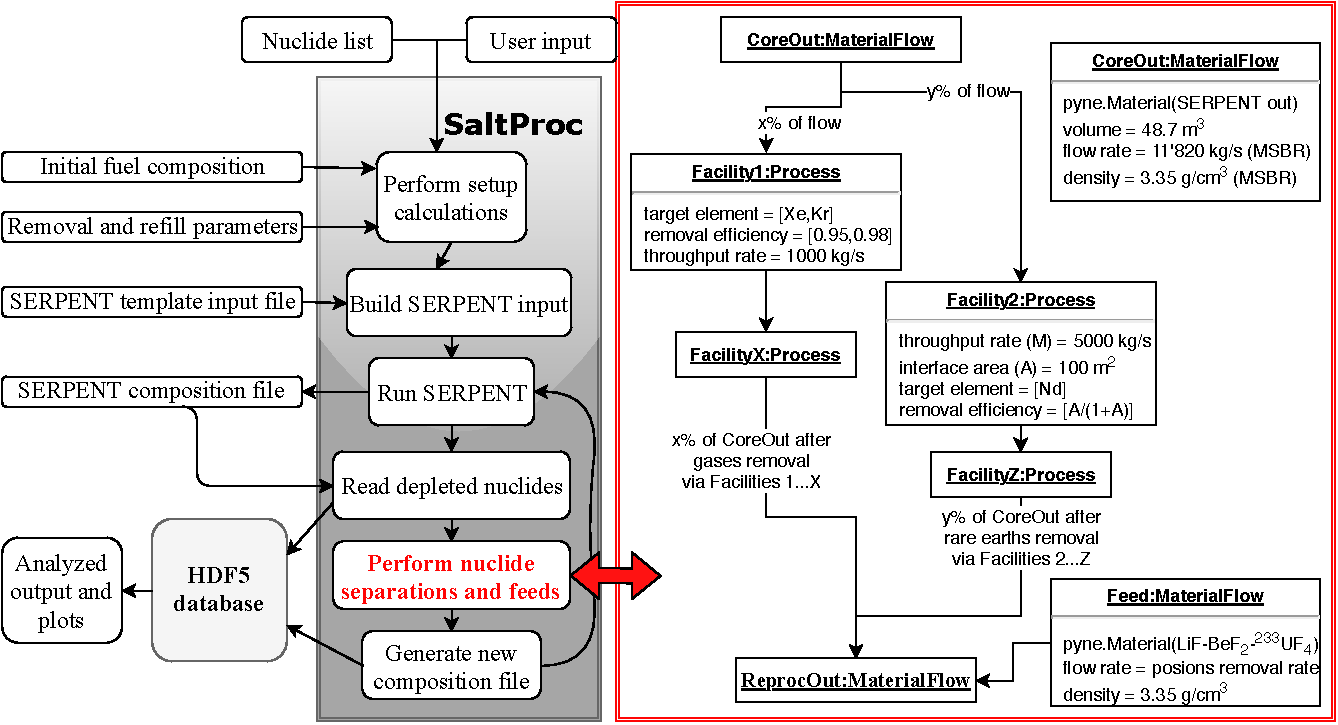
\includegraphics[width=\textwidth]{saltproc_flowchart.pdf}
  \caption{Flow chart for the Saltproc python-based tools.}
  \vspace{-1.0em}
  \label{fig:saltproc_flow}
\end{figure}
\FloatBarrier

In addition, SaltProc is able to define time-dependent material feed and removal rates to investigate the their impacts. These rates need not be constant in SaltProc. They can be defined as piecewise functions or set to respond conditions in the core. For instance, SaltProc might increase the fissile material feeding rate if the effective multiplication factor, $k_{eff}$, falls below a specific limit (e.g., 1.002). 
%Moreover, it could be useful to keep fissile material number density in the %core approximately constant to accumulated excess of $^{233}$U into the %protactinium decay tank. 
These capabilities allow SaltProc to analyze fuel cycle of a generic liquid-fueled \gls{MSR}. In summary, the development approach of SaltProc focused on producing a generic and flexible tool to give the SERPENT 2 Monte Carlo code the ability to conduct advanced fuel cycle analysis as well as simulate a myriad of online refueled systems.

%\chapter[Results]{Results}

This chapter presents calculation results based on the methodology described in Chapters 3 and 4. The effective multiplication factor, number density of major isotopes, and $^{232}$Th refill rate are calculated using a full-core SERPENT 2 model with 3-day depletion steps over a 20-year operation. Moreover, neutron flux, neutron energy spectrum, temperature reactivity coefficients, control rod worth, power density, and $^{233}$U breeding density distribution are presented for both initial and equilibrium fuel salt composition. The neutron flux and energy spectrum are calculated for the full-core model, normalized by neutron lethargy and reported for each zone. The temperature coefficients of reactivity for both the fuel salt and graphite components are estimated at the initial state by comparing effective multiplication factors at temperatures uniformly distributed from 900K and 1000K. The rod worth is calculated at several different insertion levels of control and safety rods. Finally, six factor analysis was performed to show evolution of these parameters during reactor operation.

The neutron population per cycle and the number of active/inactive cycles were chosen to obtain balance between reasonable uncertainty for a transport problem ($\leq$ 40 pcm for effective multiplication factor) and computational time. The \gls{MSBR} depletion and safety parameter computations were performed on 64 Blue Waters XK7 nodes (two AMD 6276 Interlagos CPU per node, 16 floating-point Bulldozer core units per node or 32 ``integer" cores per node, nominal clock speed is 2.45 GHz). The total computational time for achieving equilibrium composition was approximately 9,000 node hours (144,000 core hours.)

\section{Effective multiplication factor}
Figure~\ref{fig:keff} demonstrates the effective multiplication factors obtained using SaltProc and SERPENT 2. The effective multiplication factors are calculated after removing fission products listed in Table~\ref{tab:reprocessing_list} and adding the fertile material at the end of ``cycle time"\footnote{The \gls{MSBR} program defined a ``cycle time" as the amount of time required to remove 100\% of a target nuclide from a fuel salt.} which was fixed at 3 days for this work. The effective multiplication factor fluctuates significantly as a result of the batch-wise nature of this online reprocessing strategy. 
\begin{figure}[hbp!] % replace 't' with 'b' to 
  \centering
  \vspace{-0.3em}
  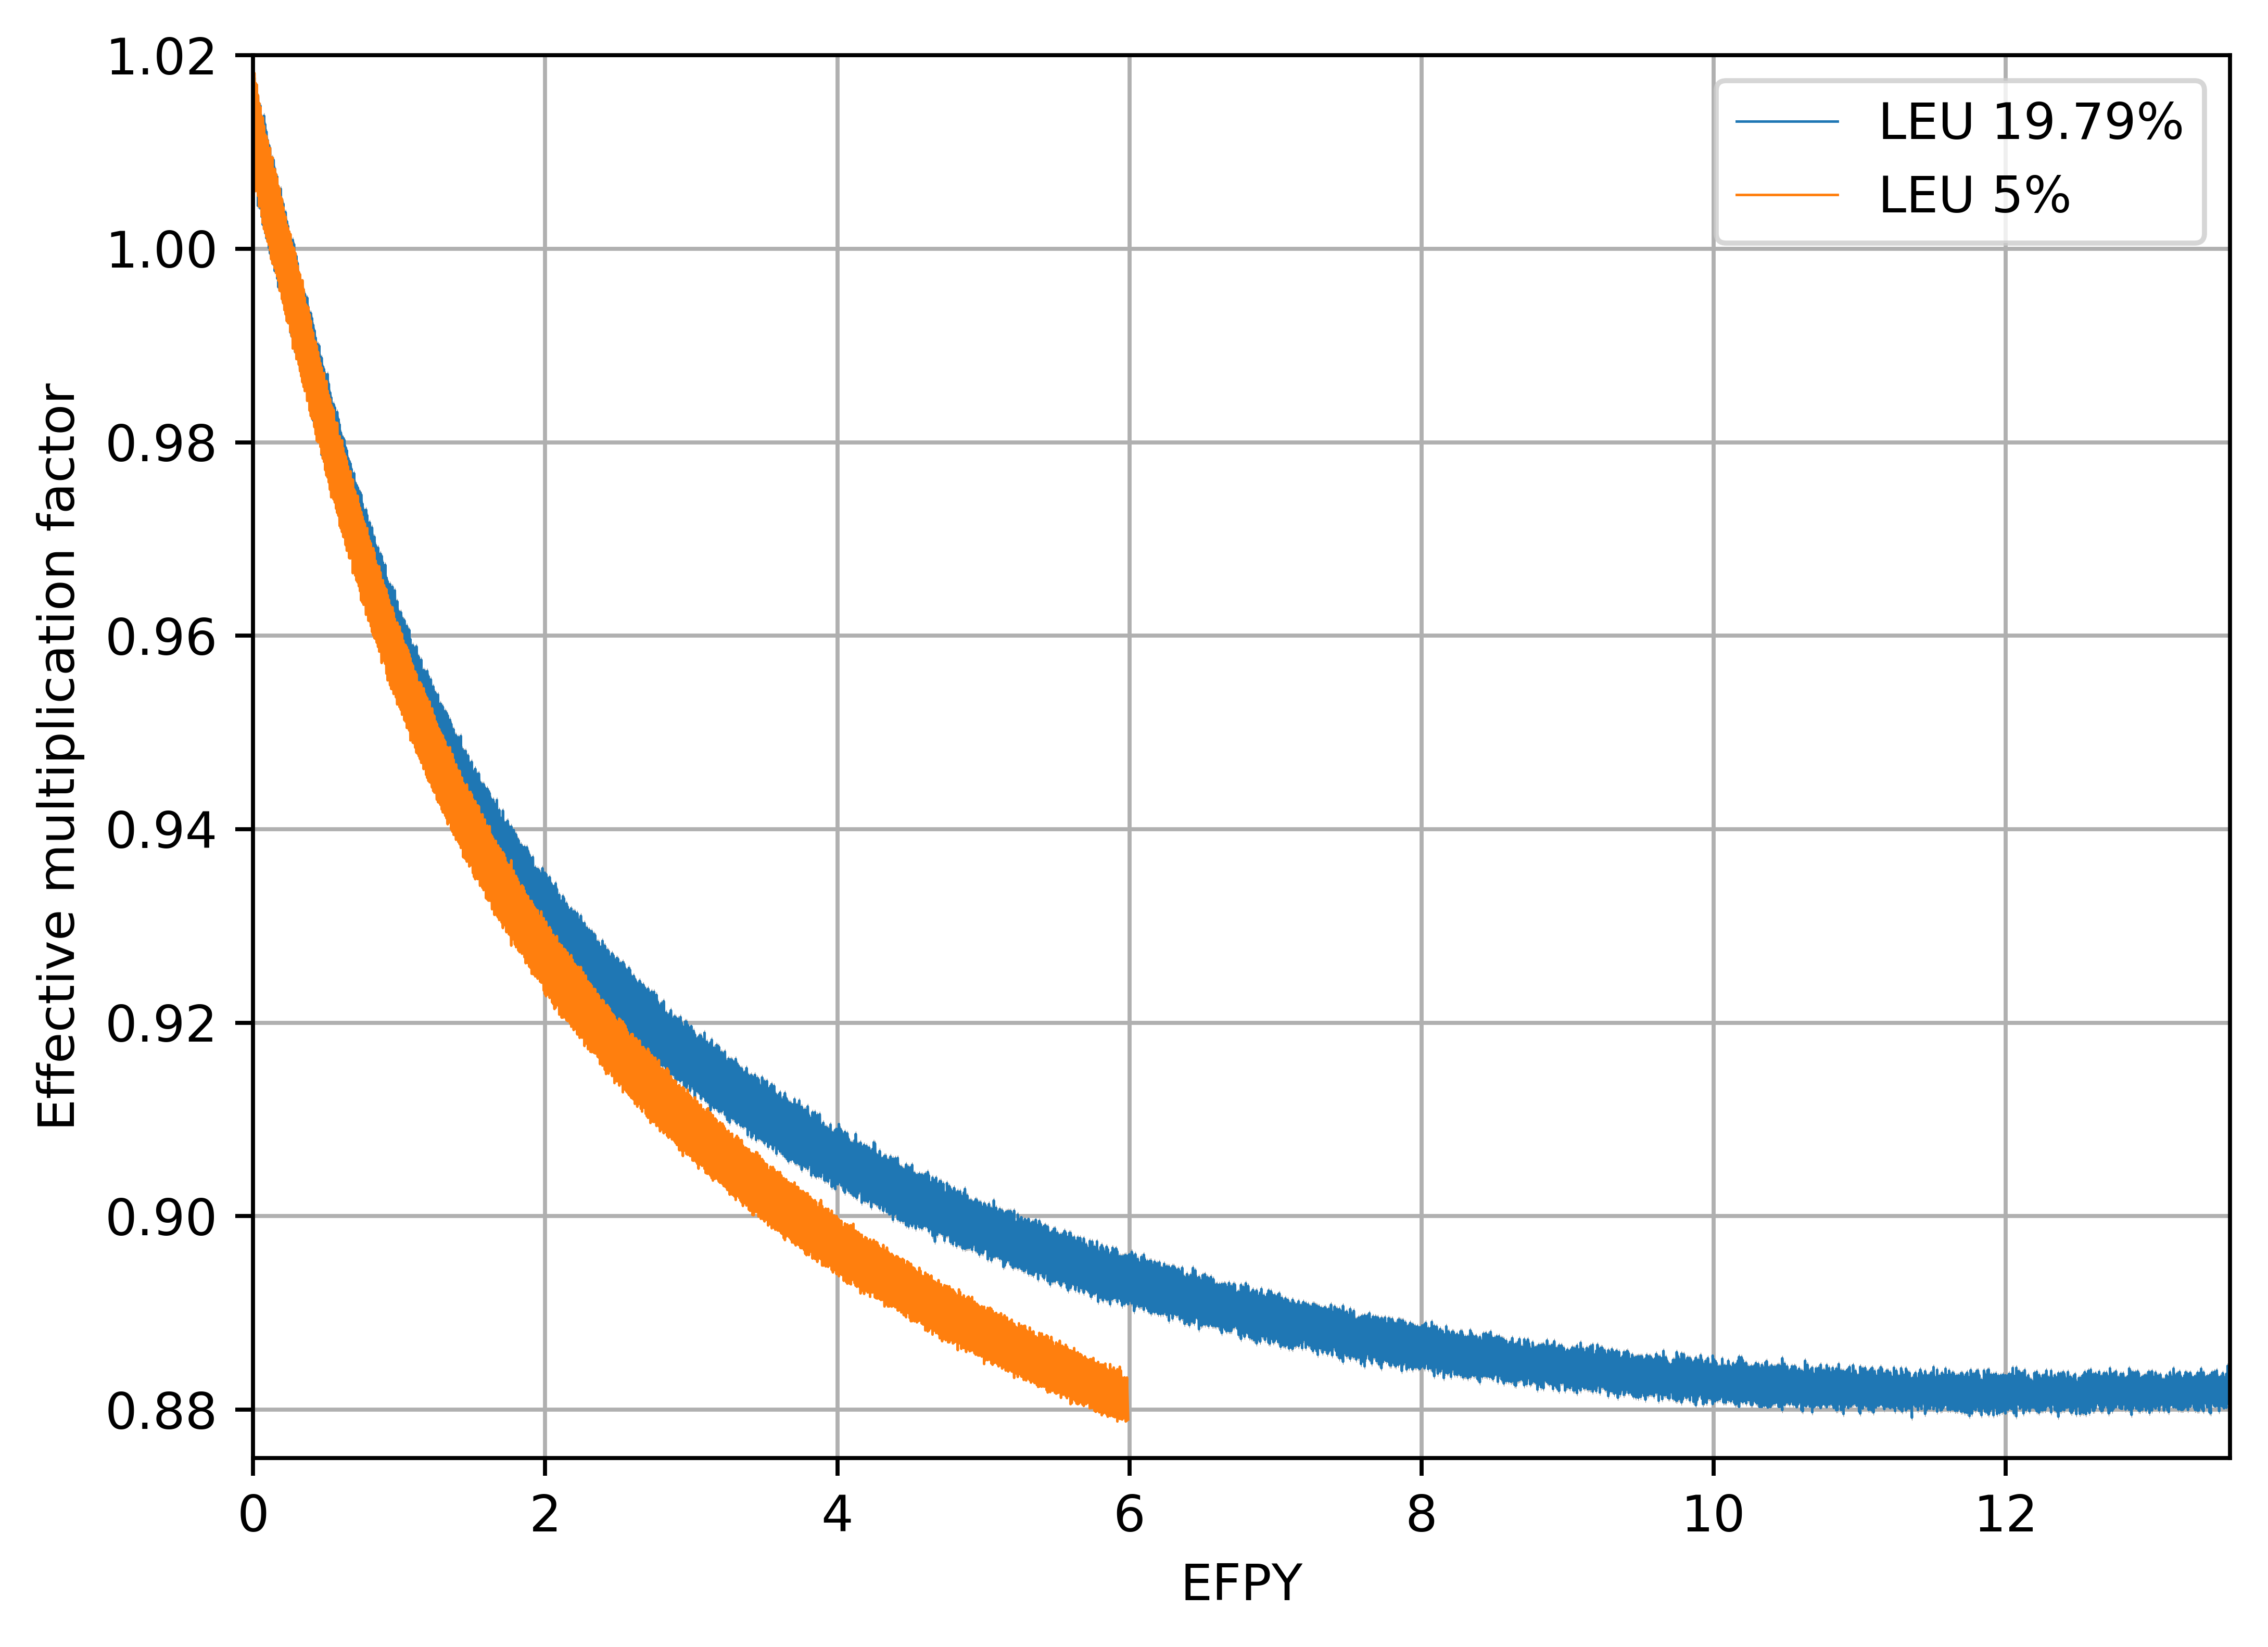
\includegraphics[width=\textwidth]{keff.png}
  \caption{Effective multiplication factor dynamics for full-core \gls{MSBR} model for a 20-year reactor operation. The confidence interval $\pm\sigma$ is shaded.}
  \vspace{-0.6em}
  \label{fig:keff}
\end{figure}
\FloatBarrier

First, SERPENT calculates the effective multiplication factor for the beginning of cycle time (fresh fuel composition for the first step). Next, it computes the new fuel salt composition for the end of a 3-day depletion step. The corresponding effective multiplication factor is much smaller than the previous one. Finally, SERPENT calculates $k_{eff}$ for the depleted composition after applying feeds and removals, and this increases accordingly since major reactor poisons (e.g. Xe, Kr) are removed, while fresh fissile material ($^{233}$U) from the protactinium decay tank is added. 

Additionaly, the presence of rubidium, strontium, cesium, and barium in the core are disadvantageous to reactor physics. In fact, removal of these elements every 3435 days causes the multiplication factor to jump by approximately 450 pcm, and limits using the batch approach for online reprocessing simulation. Overall, the effective multiplication factor gradually decreases from 1.075 to $k_{eff} \approx 1.02$ at equilibrium after approximately 6 years of irradiation. 

The analysis of the fuel salt composition evolution provides more comprehensive information about the equilibrium state. Figure~\ref{fig:adens_eq} shows major nuclides which have a strong influence on the reactor core physics normalized separately for each isotope by average atomic density, at the beginning of each depletion time step. Concentration of $^{233}$U, $^{232}$Th, $^{233}$Pa, and $^{232}$Pa in fuel salt change insignificantly after approximately 2500 days of operation. Particularly, $^{233}$U number density fluctuates less than 0.8\% in the time interval from 16 to 20 years of operation, hence,a quasi-equlibrium state was achieved after 16 years of reactor operation.

In contrast, a wide variety of nuclides, including fissile isotopes (e.g. $^{235}$U) and non-fissile strong absorbers (e.g. $^{234}$U), keep accumulating in the core. Figures~\ref{fig:fissile_short}, \ref{fig:fissile_long} demonstrate production of short-life and long-life fissile isotopes in the core, respectively. In the end of considered operational time the core contains significant $^{235}$U ($\approx 9\times10^{-6}$ atom/b-cm), $^{238}$Pu ($\approx 10^{-6}$ atom/b-cm), $^{237}$Np ($\approx10^{-6}$ atom/b-cm), $^{232}$U ($\approx$10$^{-7}$ atom/b-cm), $^{239}$Pu ($\approx10^{-7}$ atom/b-cm), and $^{241}$Pu ($\approx 5\times10^{-8}$ atom/b-cm). Meanwhile, the equilibrium number density of the target fissile isotope $^{233}$U was approximately 7.97$\times10^{-5}$ atom/b-cm. Thus, production of new fissile materials in the core as well as $^{233}$U breeding make it possible to compensate for negative effects of strong absorber accumulation and keep the reactor critical.

\begin{figure}[htp!] % replace 't' with 'b' to 
  \centering
  \vspace{-0.3em}
  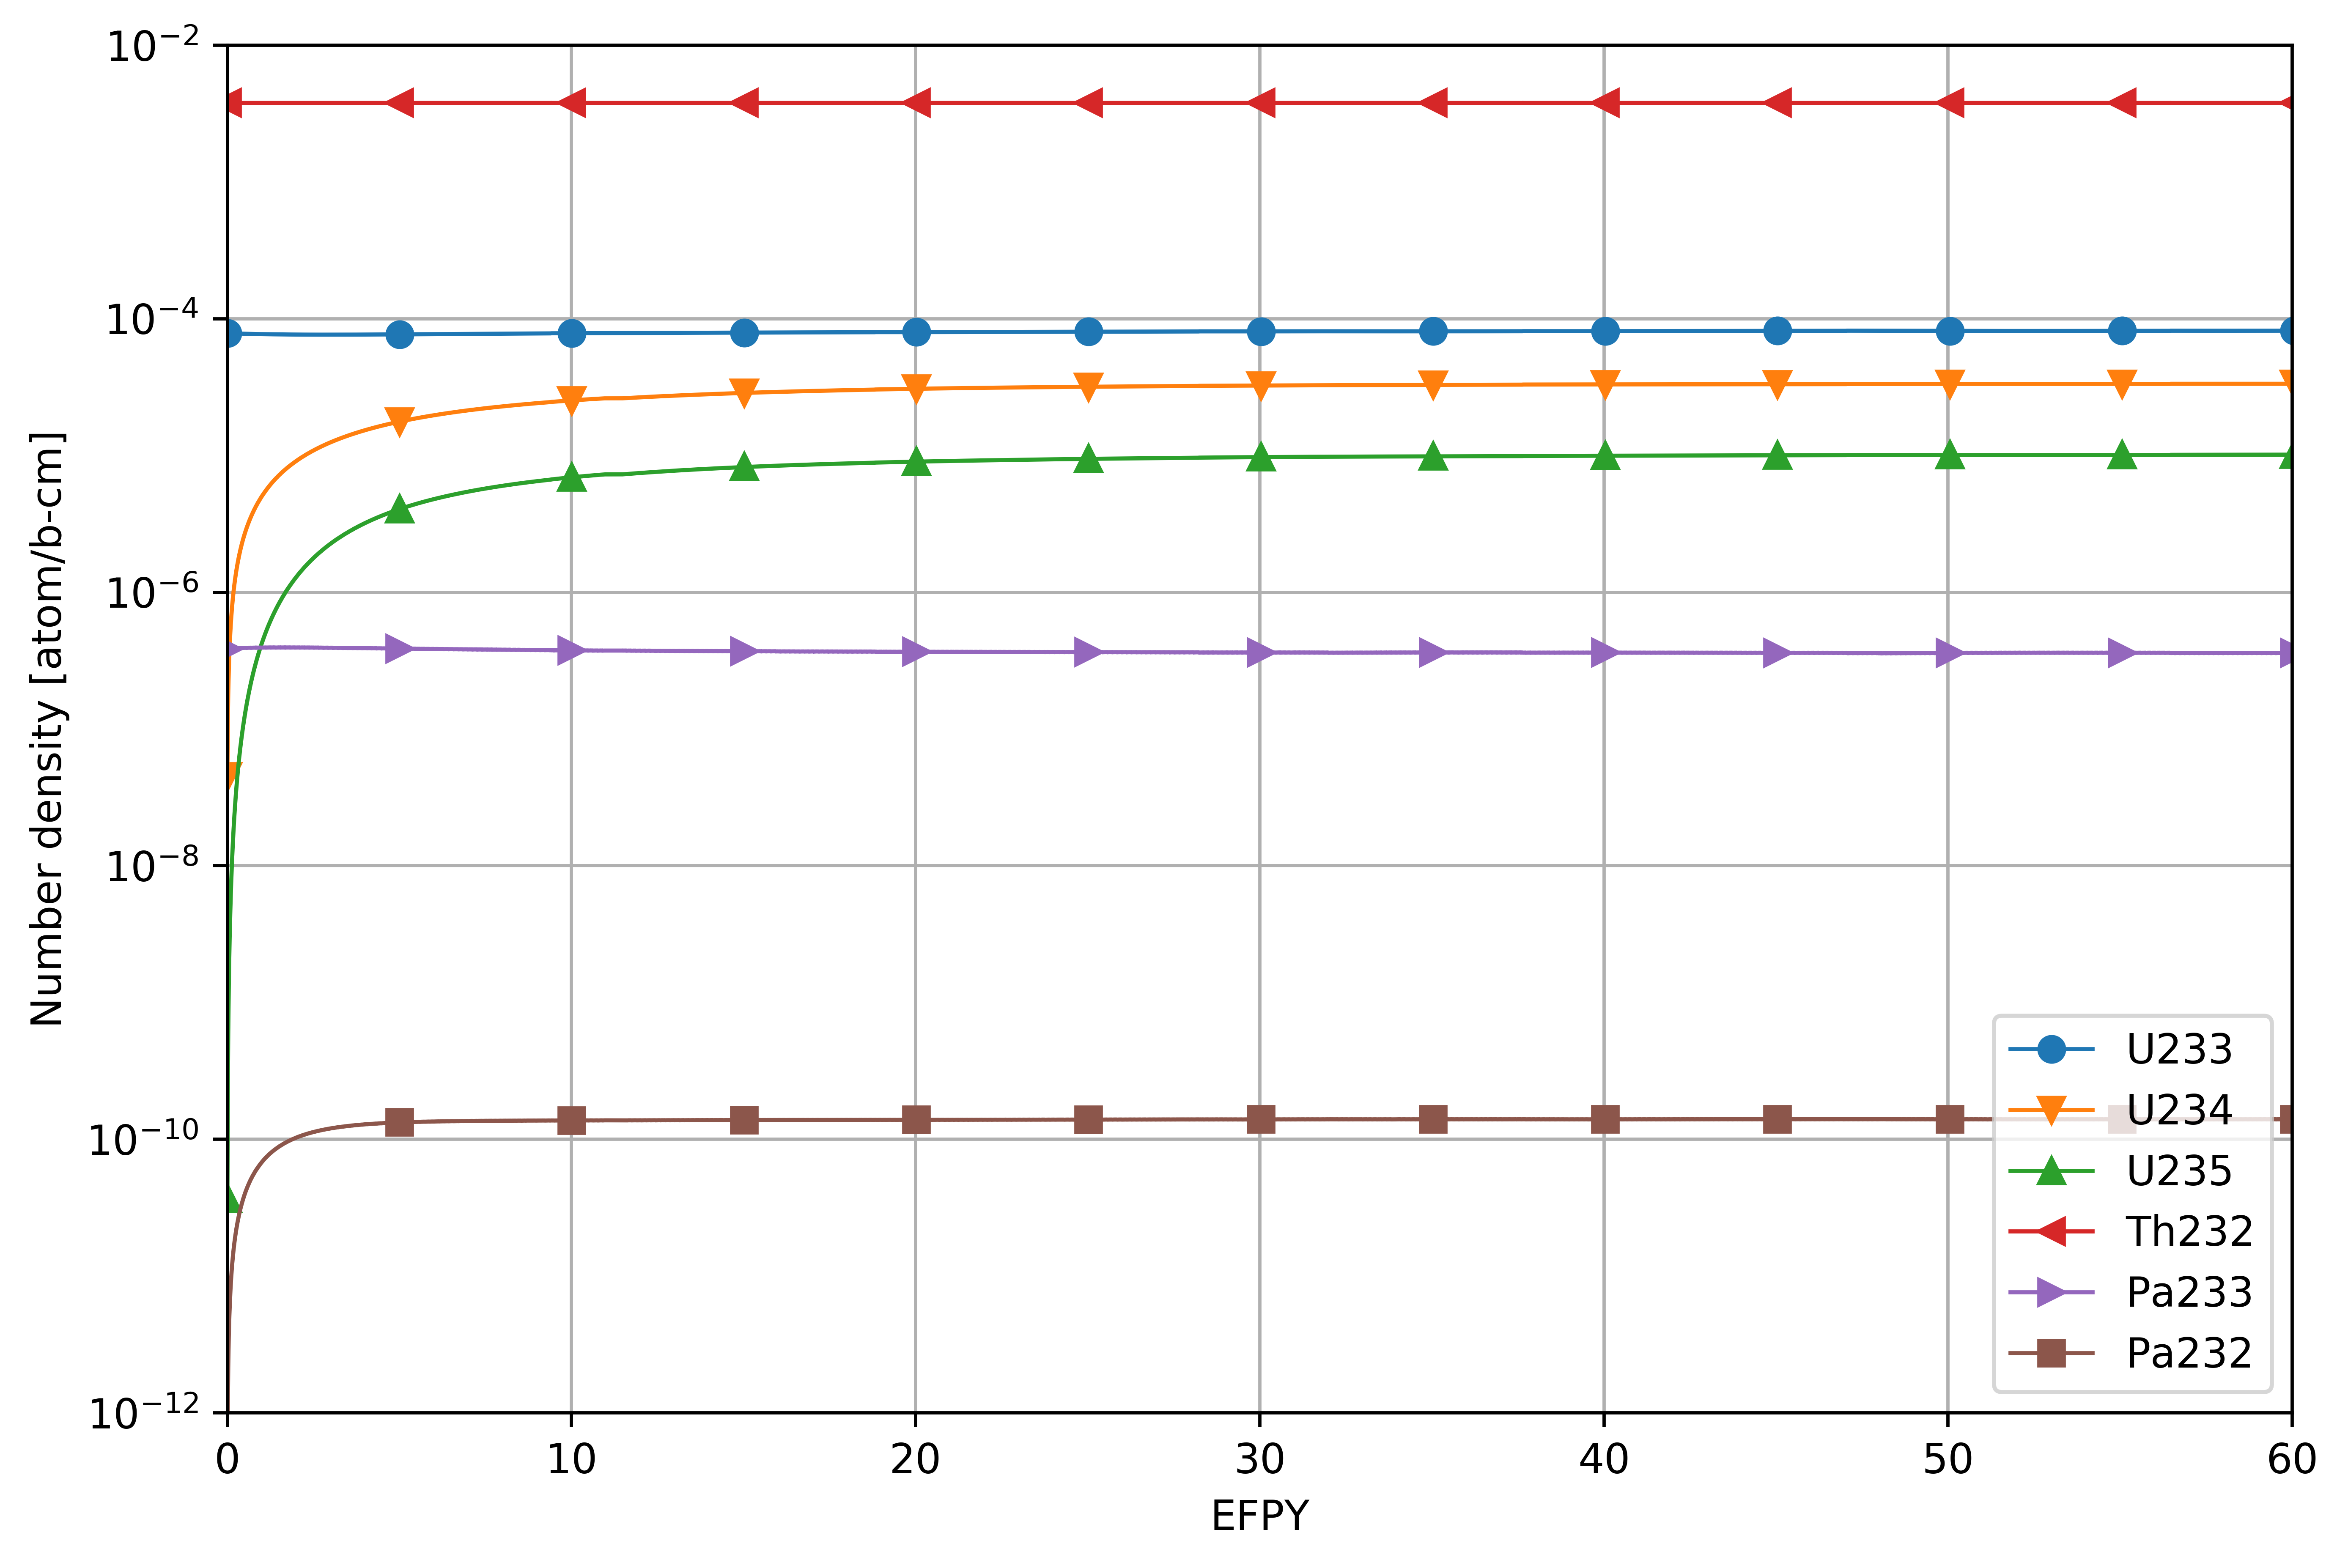
\includegraphics[width=\textwidth]{major_isotopes_adens.png}
  \caption{Normalized number density of major nuclides during the reactor operation.}
  \vspace{-0.6em}
  \label{fig:adens_eq}
\end{figure}
\FloatBarrier

\begin{figure}[htp!] % replace 't' with 'b' to 
  \centering
  \vspace{-1.3em}
  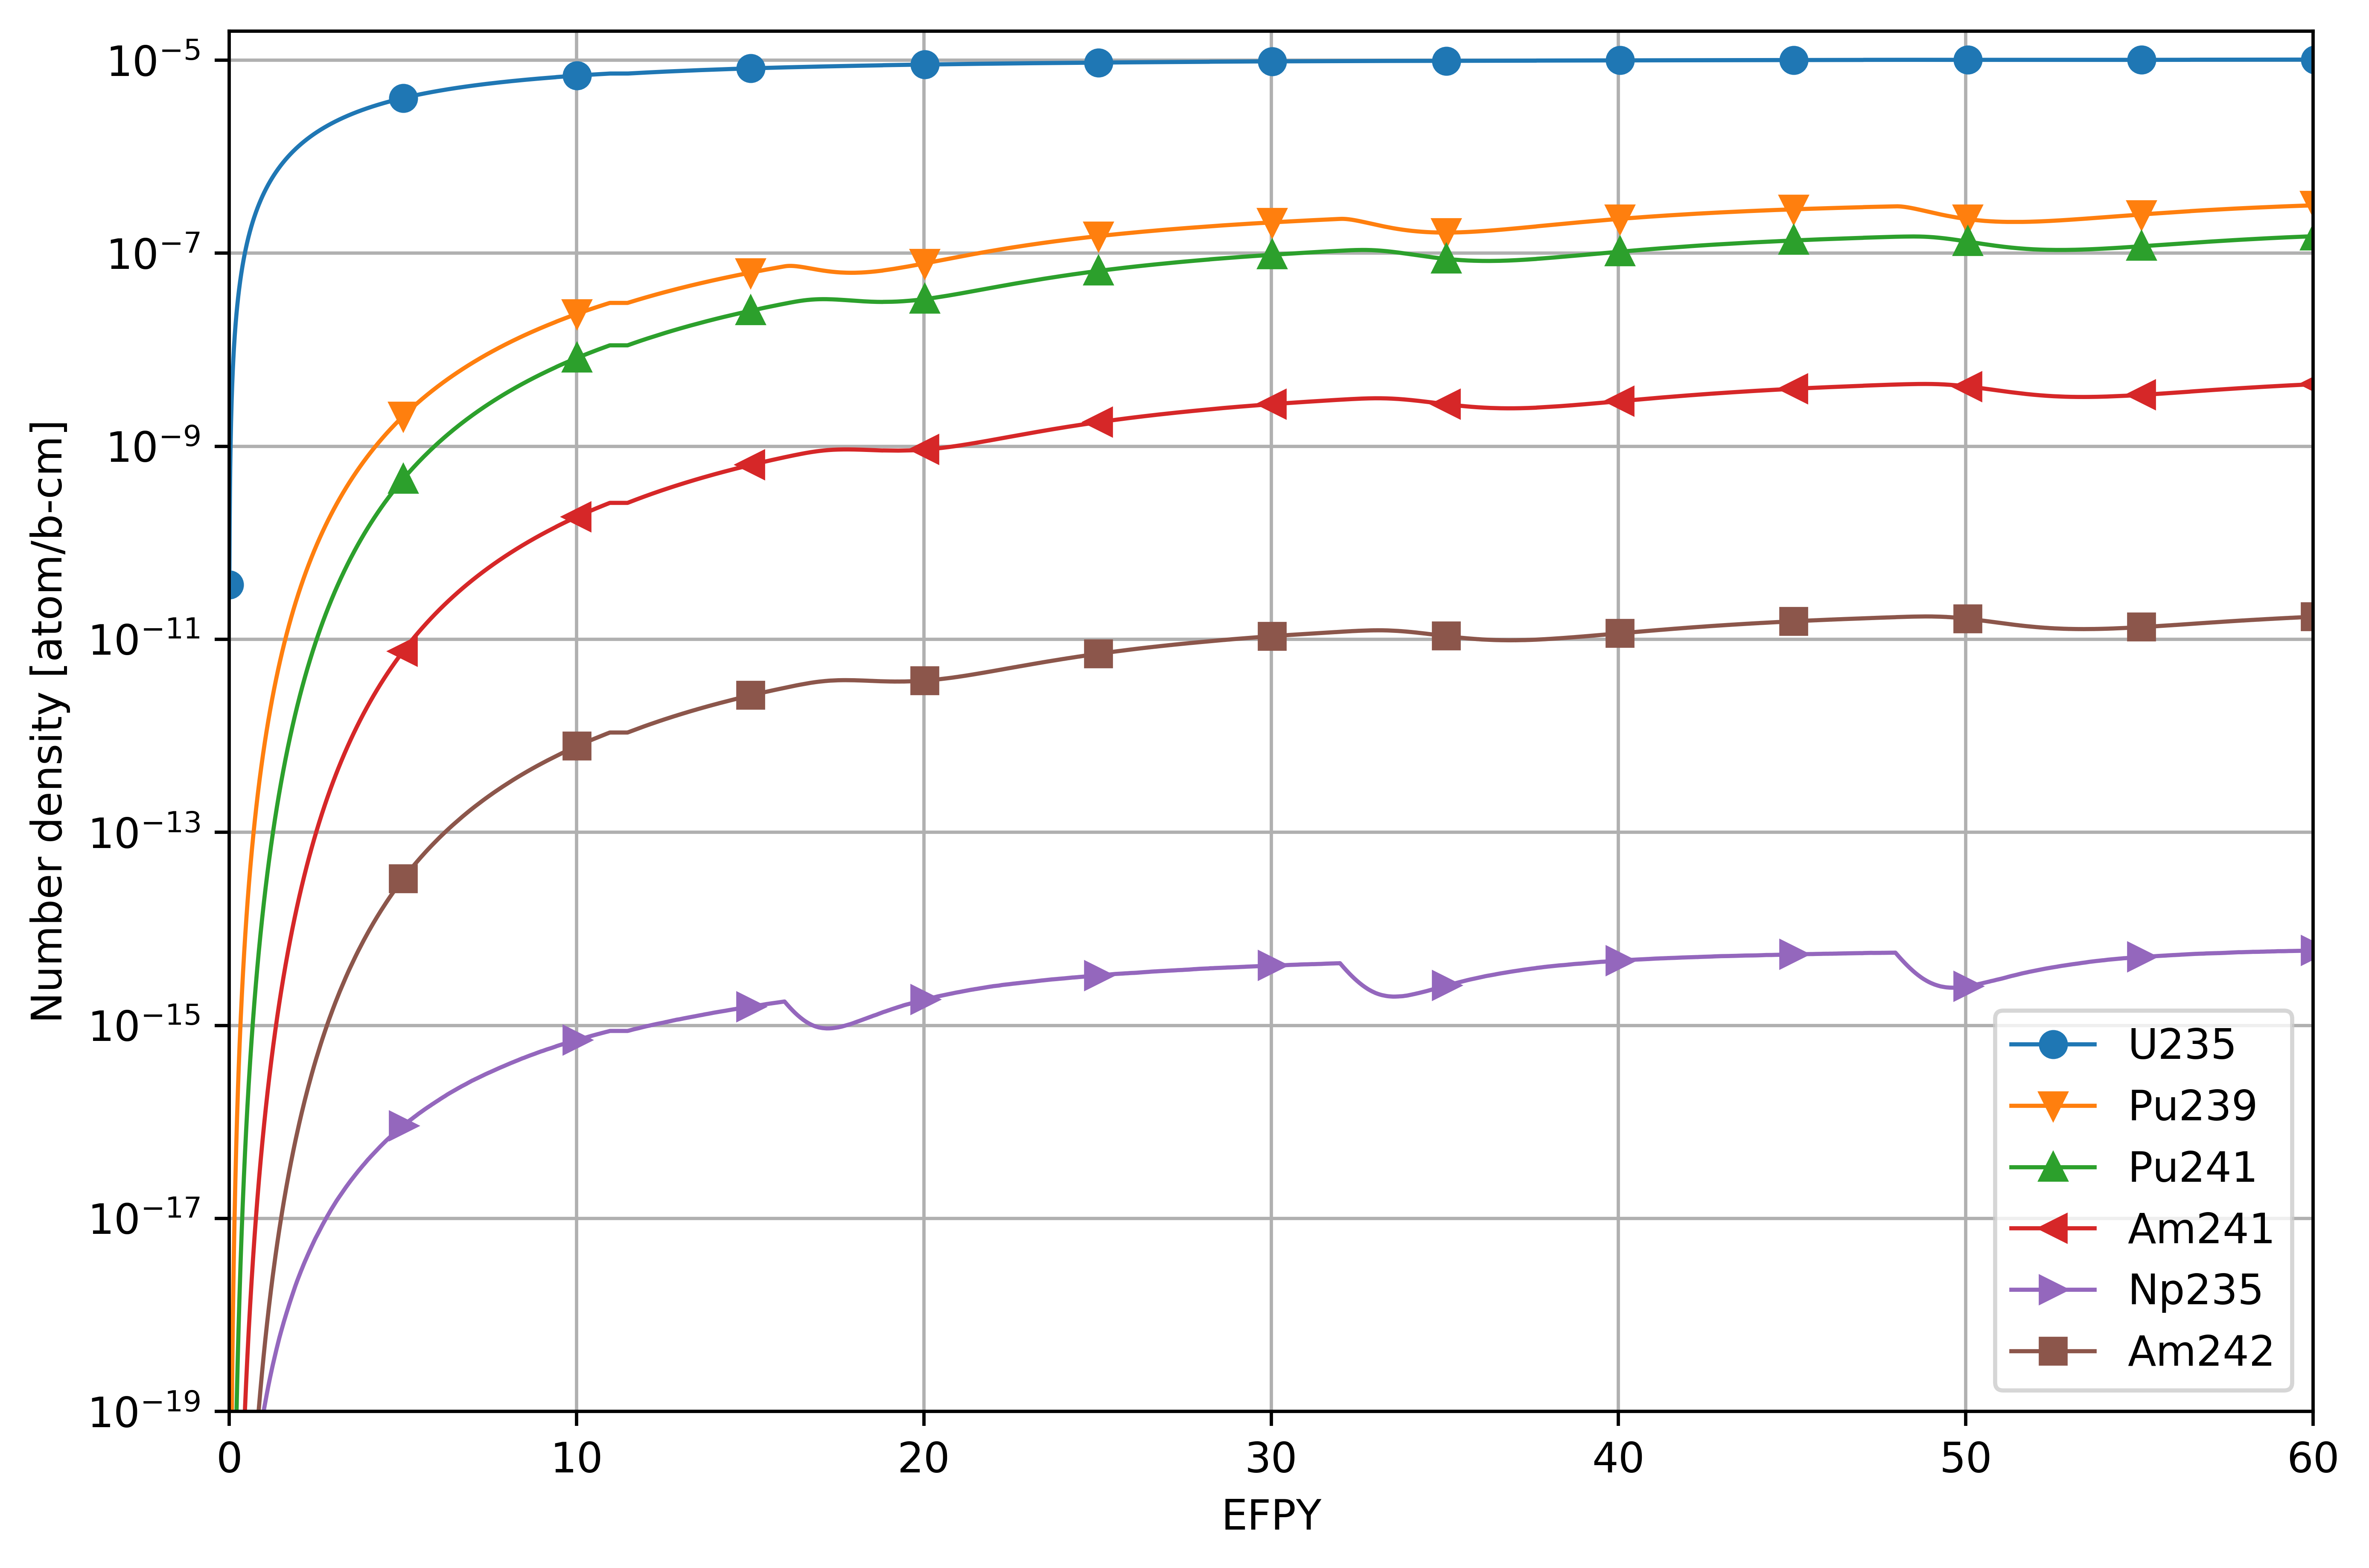
\includegraphics[width=\textwidth]{fissile_short.png}
   \vspace{-1.5em}
  \caption{Absolute number density of short-lived fissile nuclides ($\tau_{1/2}<900y$) during the reactor operation.}
  \vspace{-1.6em}
  \label{fig:fissile_short}
\end{figure}
\begin{figure}[hbp!] % replace 't' with 'b' to 
  \centering
  \vspace{-0.3em}
  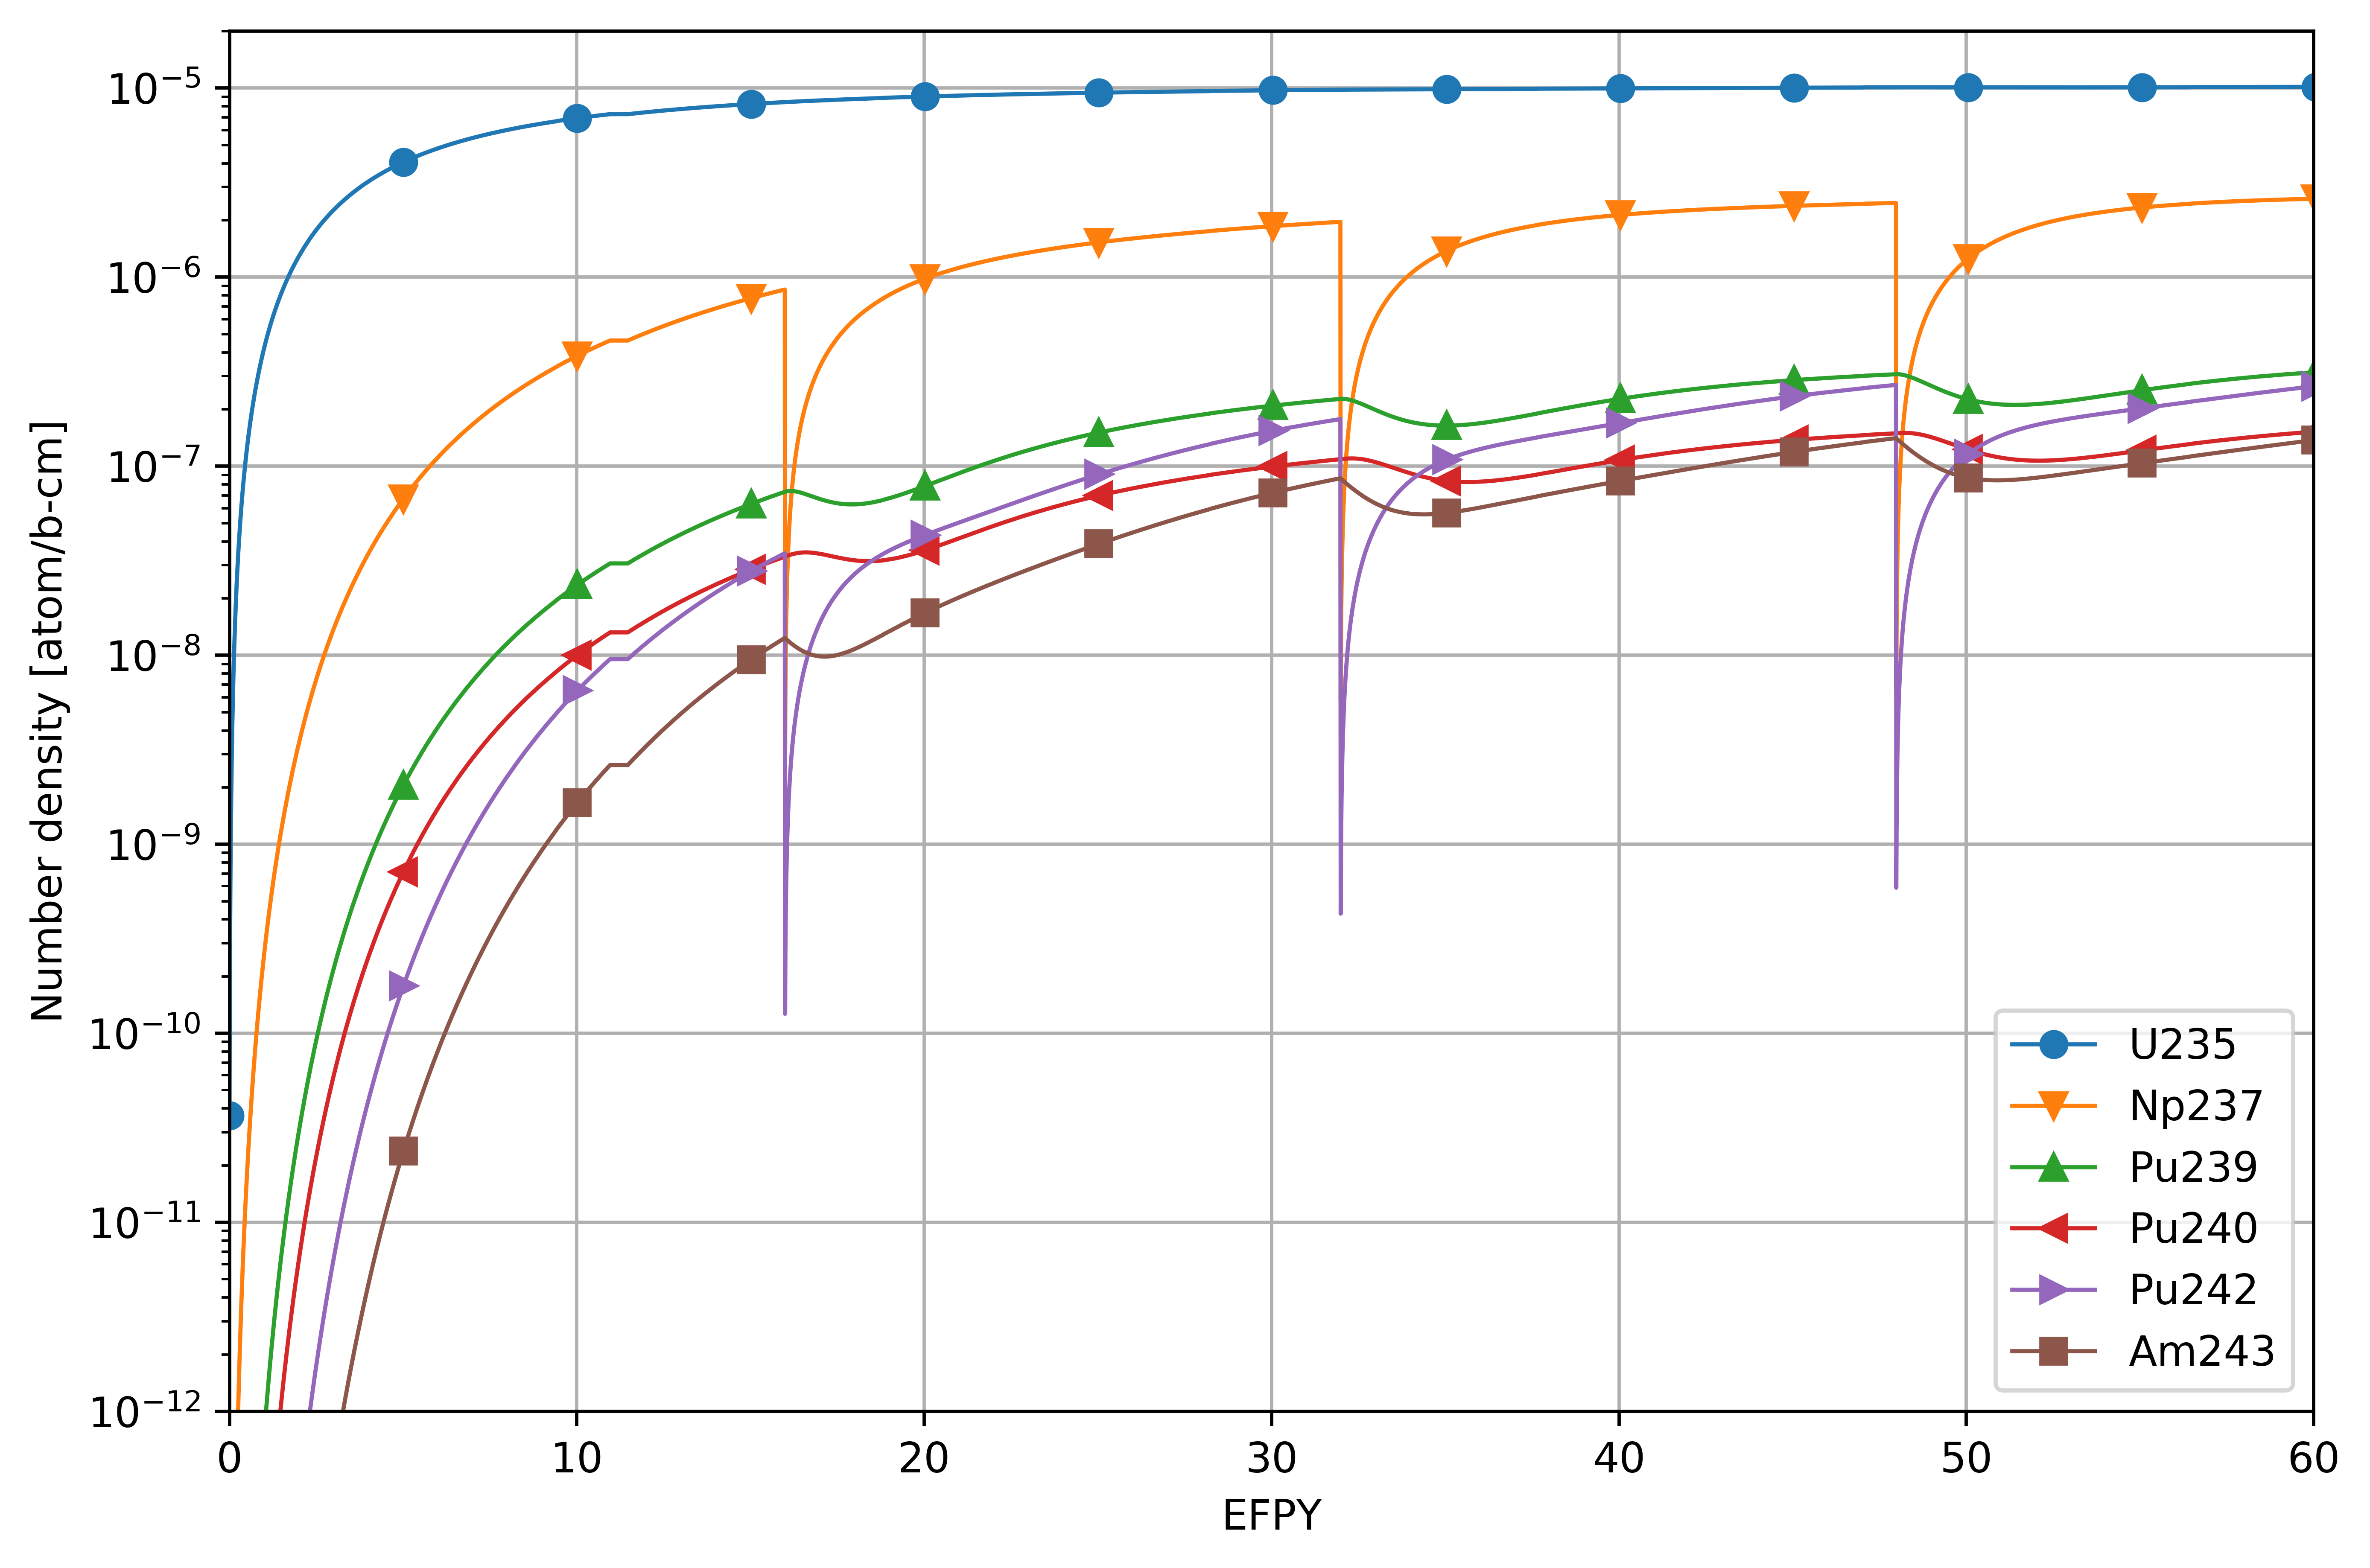
\includegraphics[width=\textwidth]{fissile_long.png}
   \vspace{-1.5em}
  \caption{Absolute number density of long-lived fissile nuclides ($\tau_{1/2}>900y$) during the reactor operation.}
  \vspace{-2.6em}
  \label{fig:fissile_long}
\end{figure}
\FloatBarrier

\section{Neutron spectrum}
Figure~\ref{fig:spectrum} shows the normalized neutron flux spectrum for the full-core \gls{MSBR} model in the energy range from $10^{-8}$ to $10$ MeV. The neutron energy spectrum at equilibrium is harder than at startup due to $^{238}$Pu, $^{239}$Pu, $^{240}$Pu, $^{241}$Pu, and $^{242}$Pu accumulation in the core during reactor operation. 

\begin{figure}[htp!] % replace 't' with 'b' to force it to 
  \centering
    \vspace{-0.3em}
  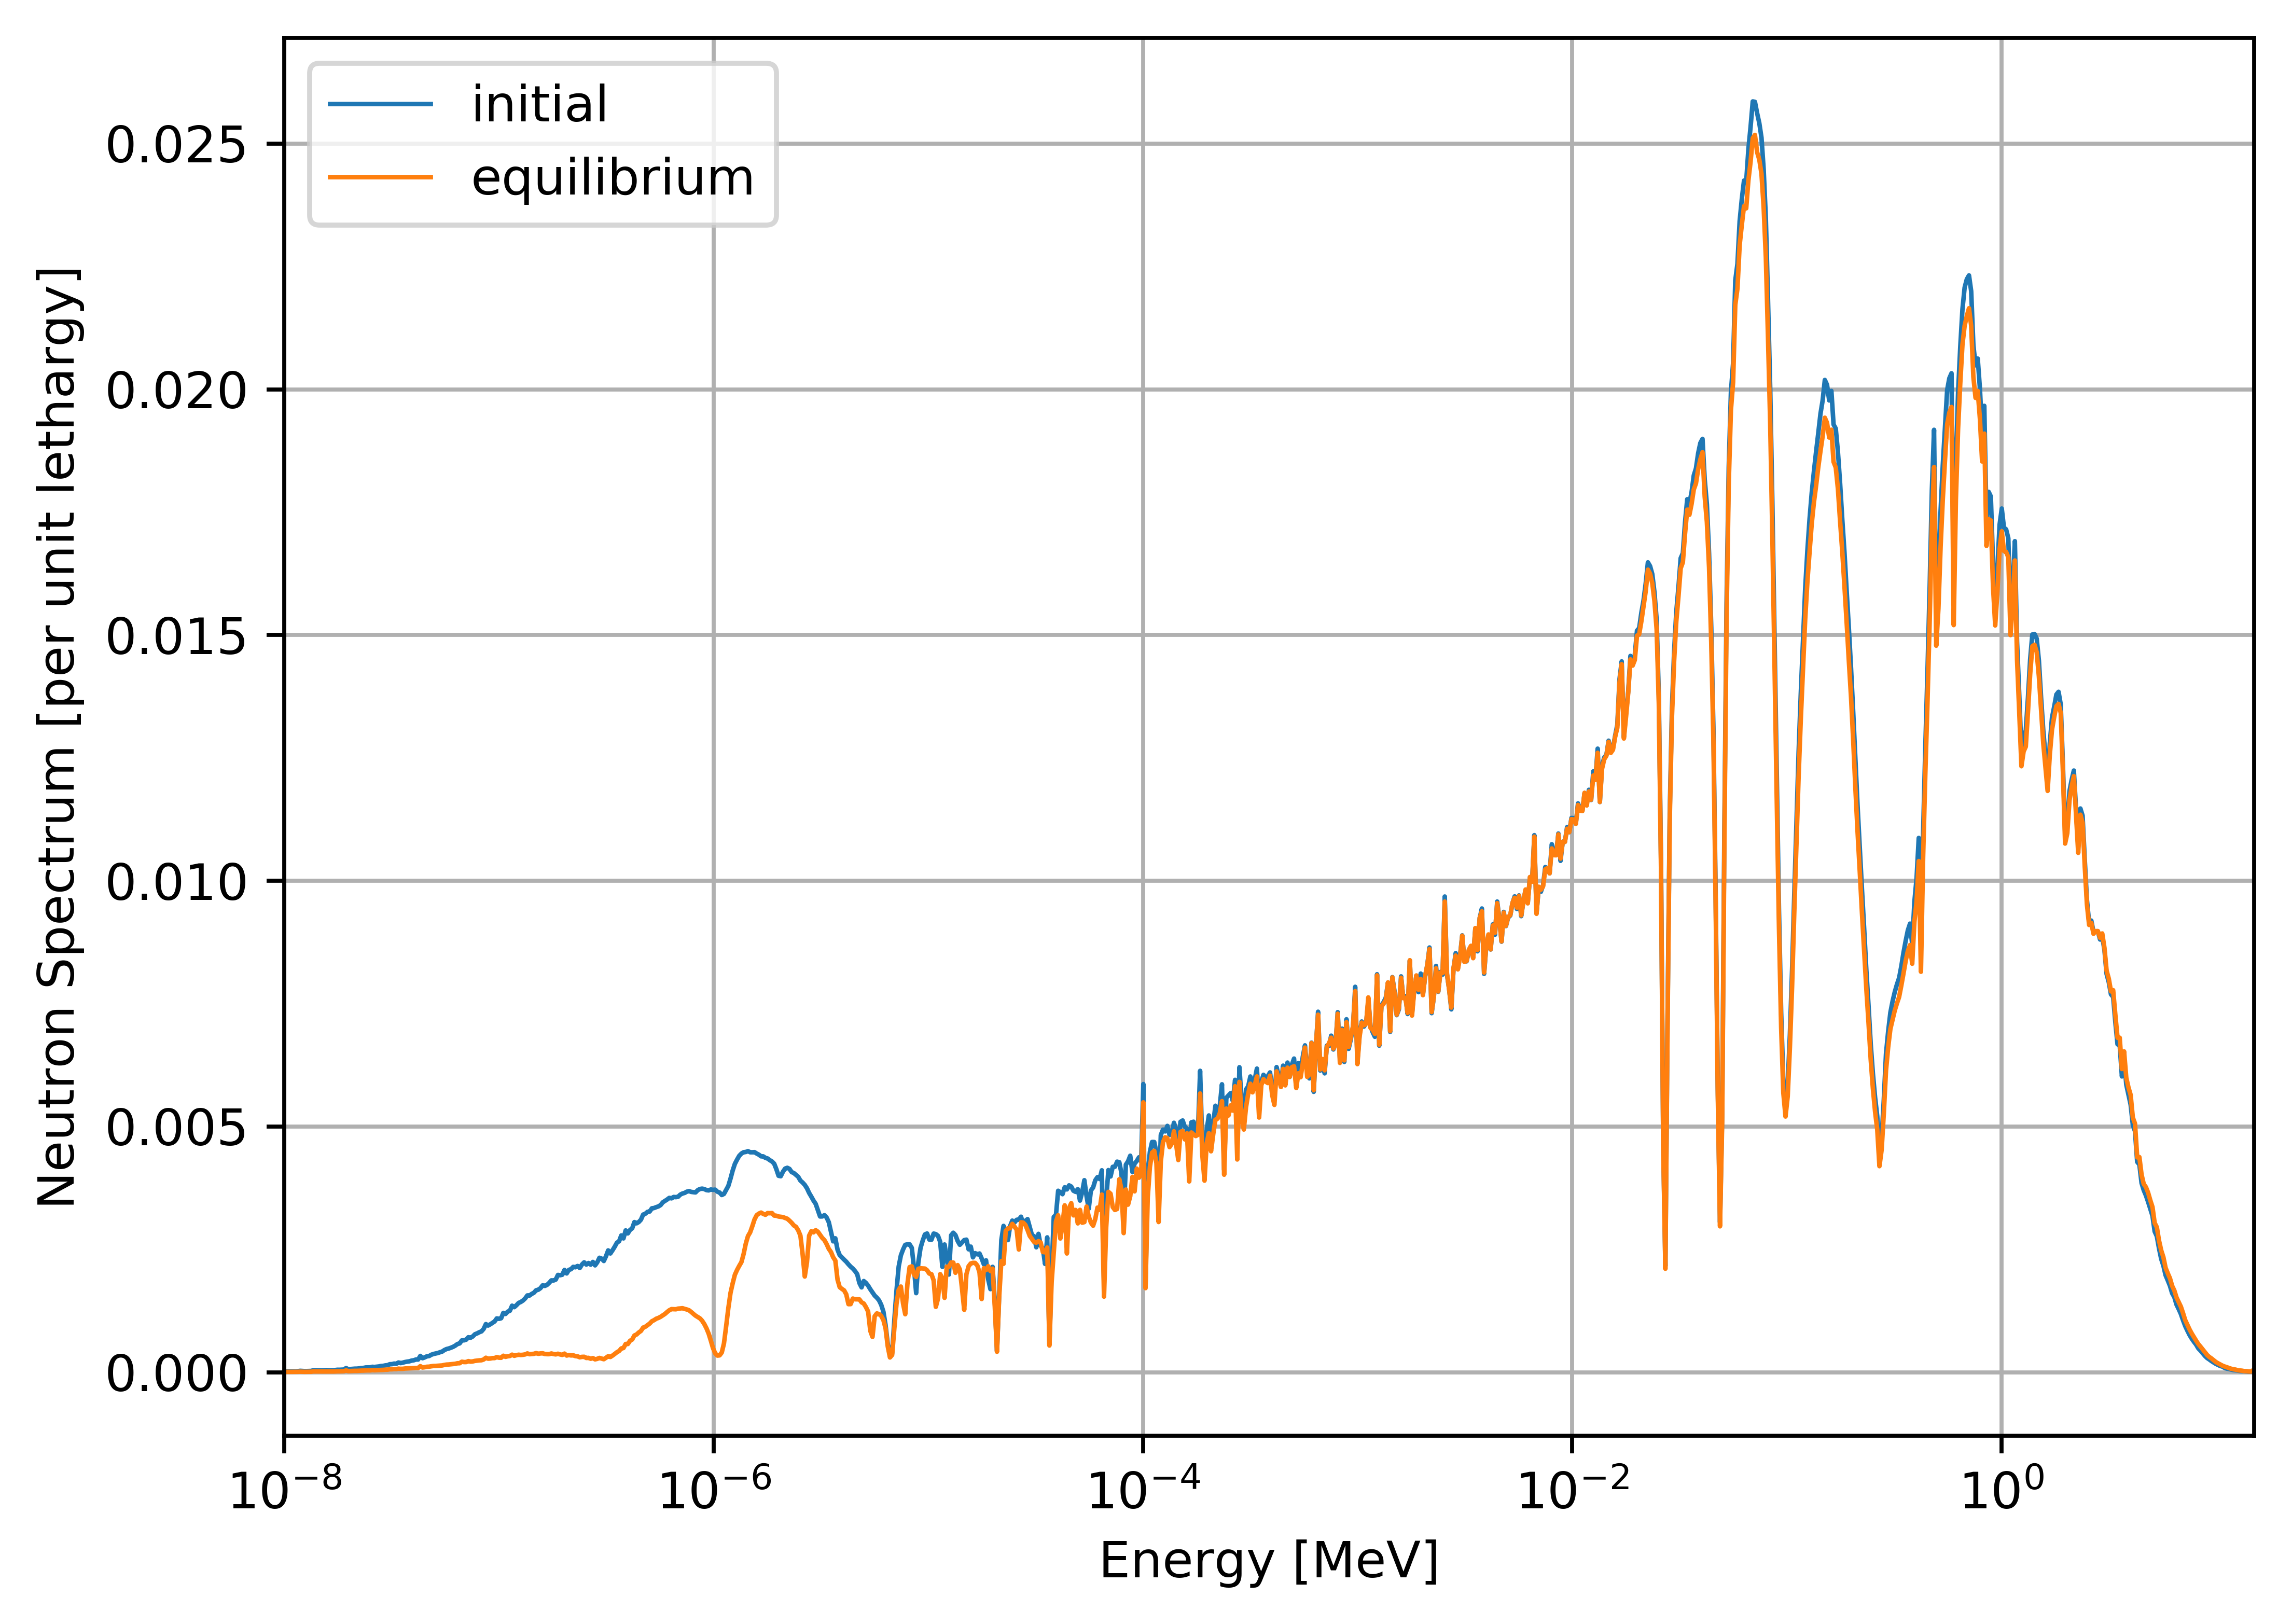
\includegraphics[width=\textwidth]{spectrum.png} 
  \caption{Neutron flux energy spectrum normalized by unit lethargy for initial and equilibrium fuel salt composition.}
    \vspace{-0.6em}
  \label{fig:spectrum}
\end{figure}
\FloatBarrier

Figure~\ref{fig:spectrum_zones_init}, \ref{fig:spectrum_zones_eq} shows that zone I produced much more thermal neutrons than zone II, indicating that the majority of fissions occured in the central part of the core. In the undermoderated zone II, the neutron energy spectrum is harder which leads to more capture of neutrons by $^{232}$Th and helps a achieve relatively high breeding ratio. Moreover, the (n,$\gamma$) resonance energy range in $^{232}$Th is from 10$^{-4}$ to 10$^{-2}$ MeV. Therefore, the moderator-to-fuel ratio for zone II was chosen to shift the neutron energy spectrum in this range. Furthermore, in the central core region (zone I), the neutron energy spectrum shifts to a harder spectrum over 20 years of reactor operation. In contrast, in the outer core region (zone II) a similar spectral shift takes place at a reduced scale. This resuls is in a good agreement with original ORNL report \cite{robertson_conceptual_1971} and most recent whole-core steady-state study \cite{park_whole_2015}.

It is important to obtain the epithermal and thermal spectra to produce $^{233}$U from $^{232}$Th because the radiative capture cross section of thorium decreases monotonically from $10^{-10}$ MeV to $10^{-5}$ MeV. Hardening the spectrum tends to significantly increase resonance absorption in thorium and decrease the absorptions in fissile and construction materials. Thus, a signficant amount fissile material will be needed to make the reactor critical. 

\begin{figure}[htp!] % replace 't' with 'b' to force it to 
  \centering
    \vspace{-0.3em}
  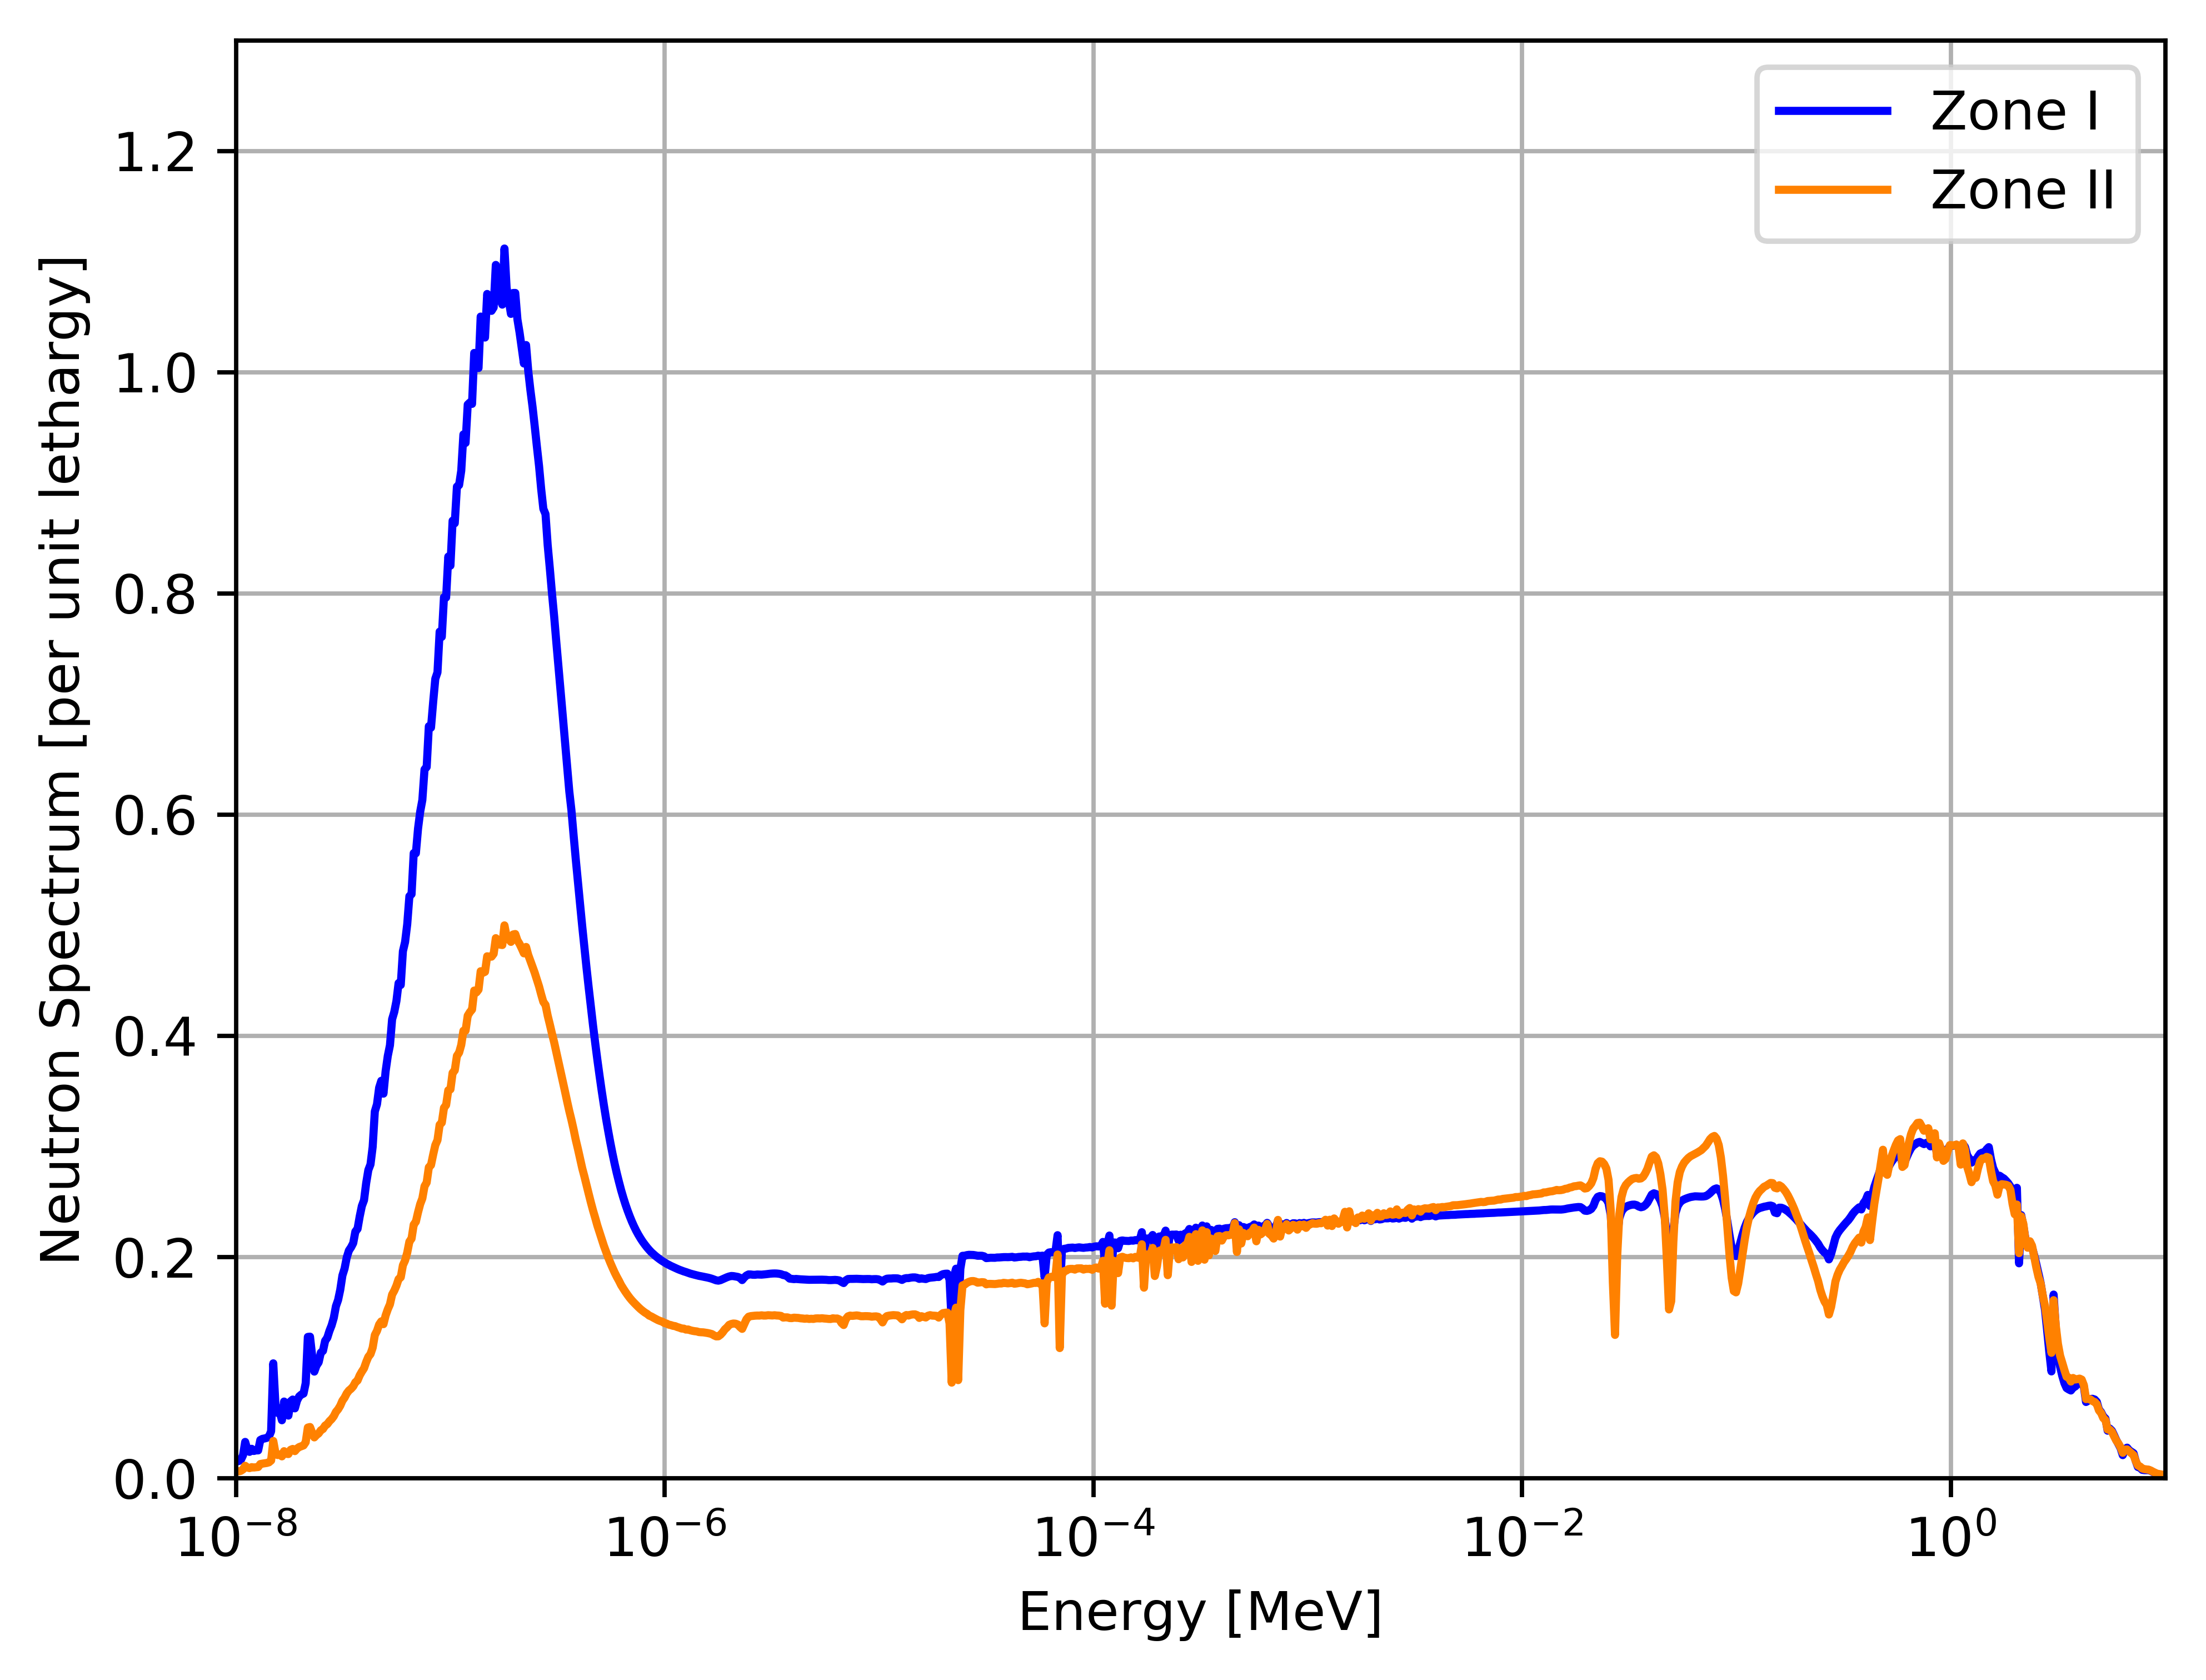
\includegraphics[width=\textwidth]{spectrum_zones_init.png} 
      \vspace{-0.3em}
  \caption{Neutron flux energy spectrum in different core regions normalized by unit lethargy for the initial fuel salt composition.}
    \vspace{-1.6em}
  \label{fig:spectrum_zones_init}
\end{figure}
\begin{figure}[htp!] % replace 't' with 'b' to force it to 
  \centering
    \vspace{-0.3em}
  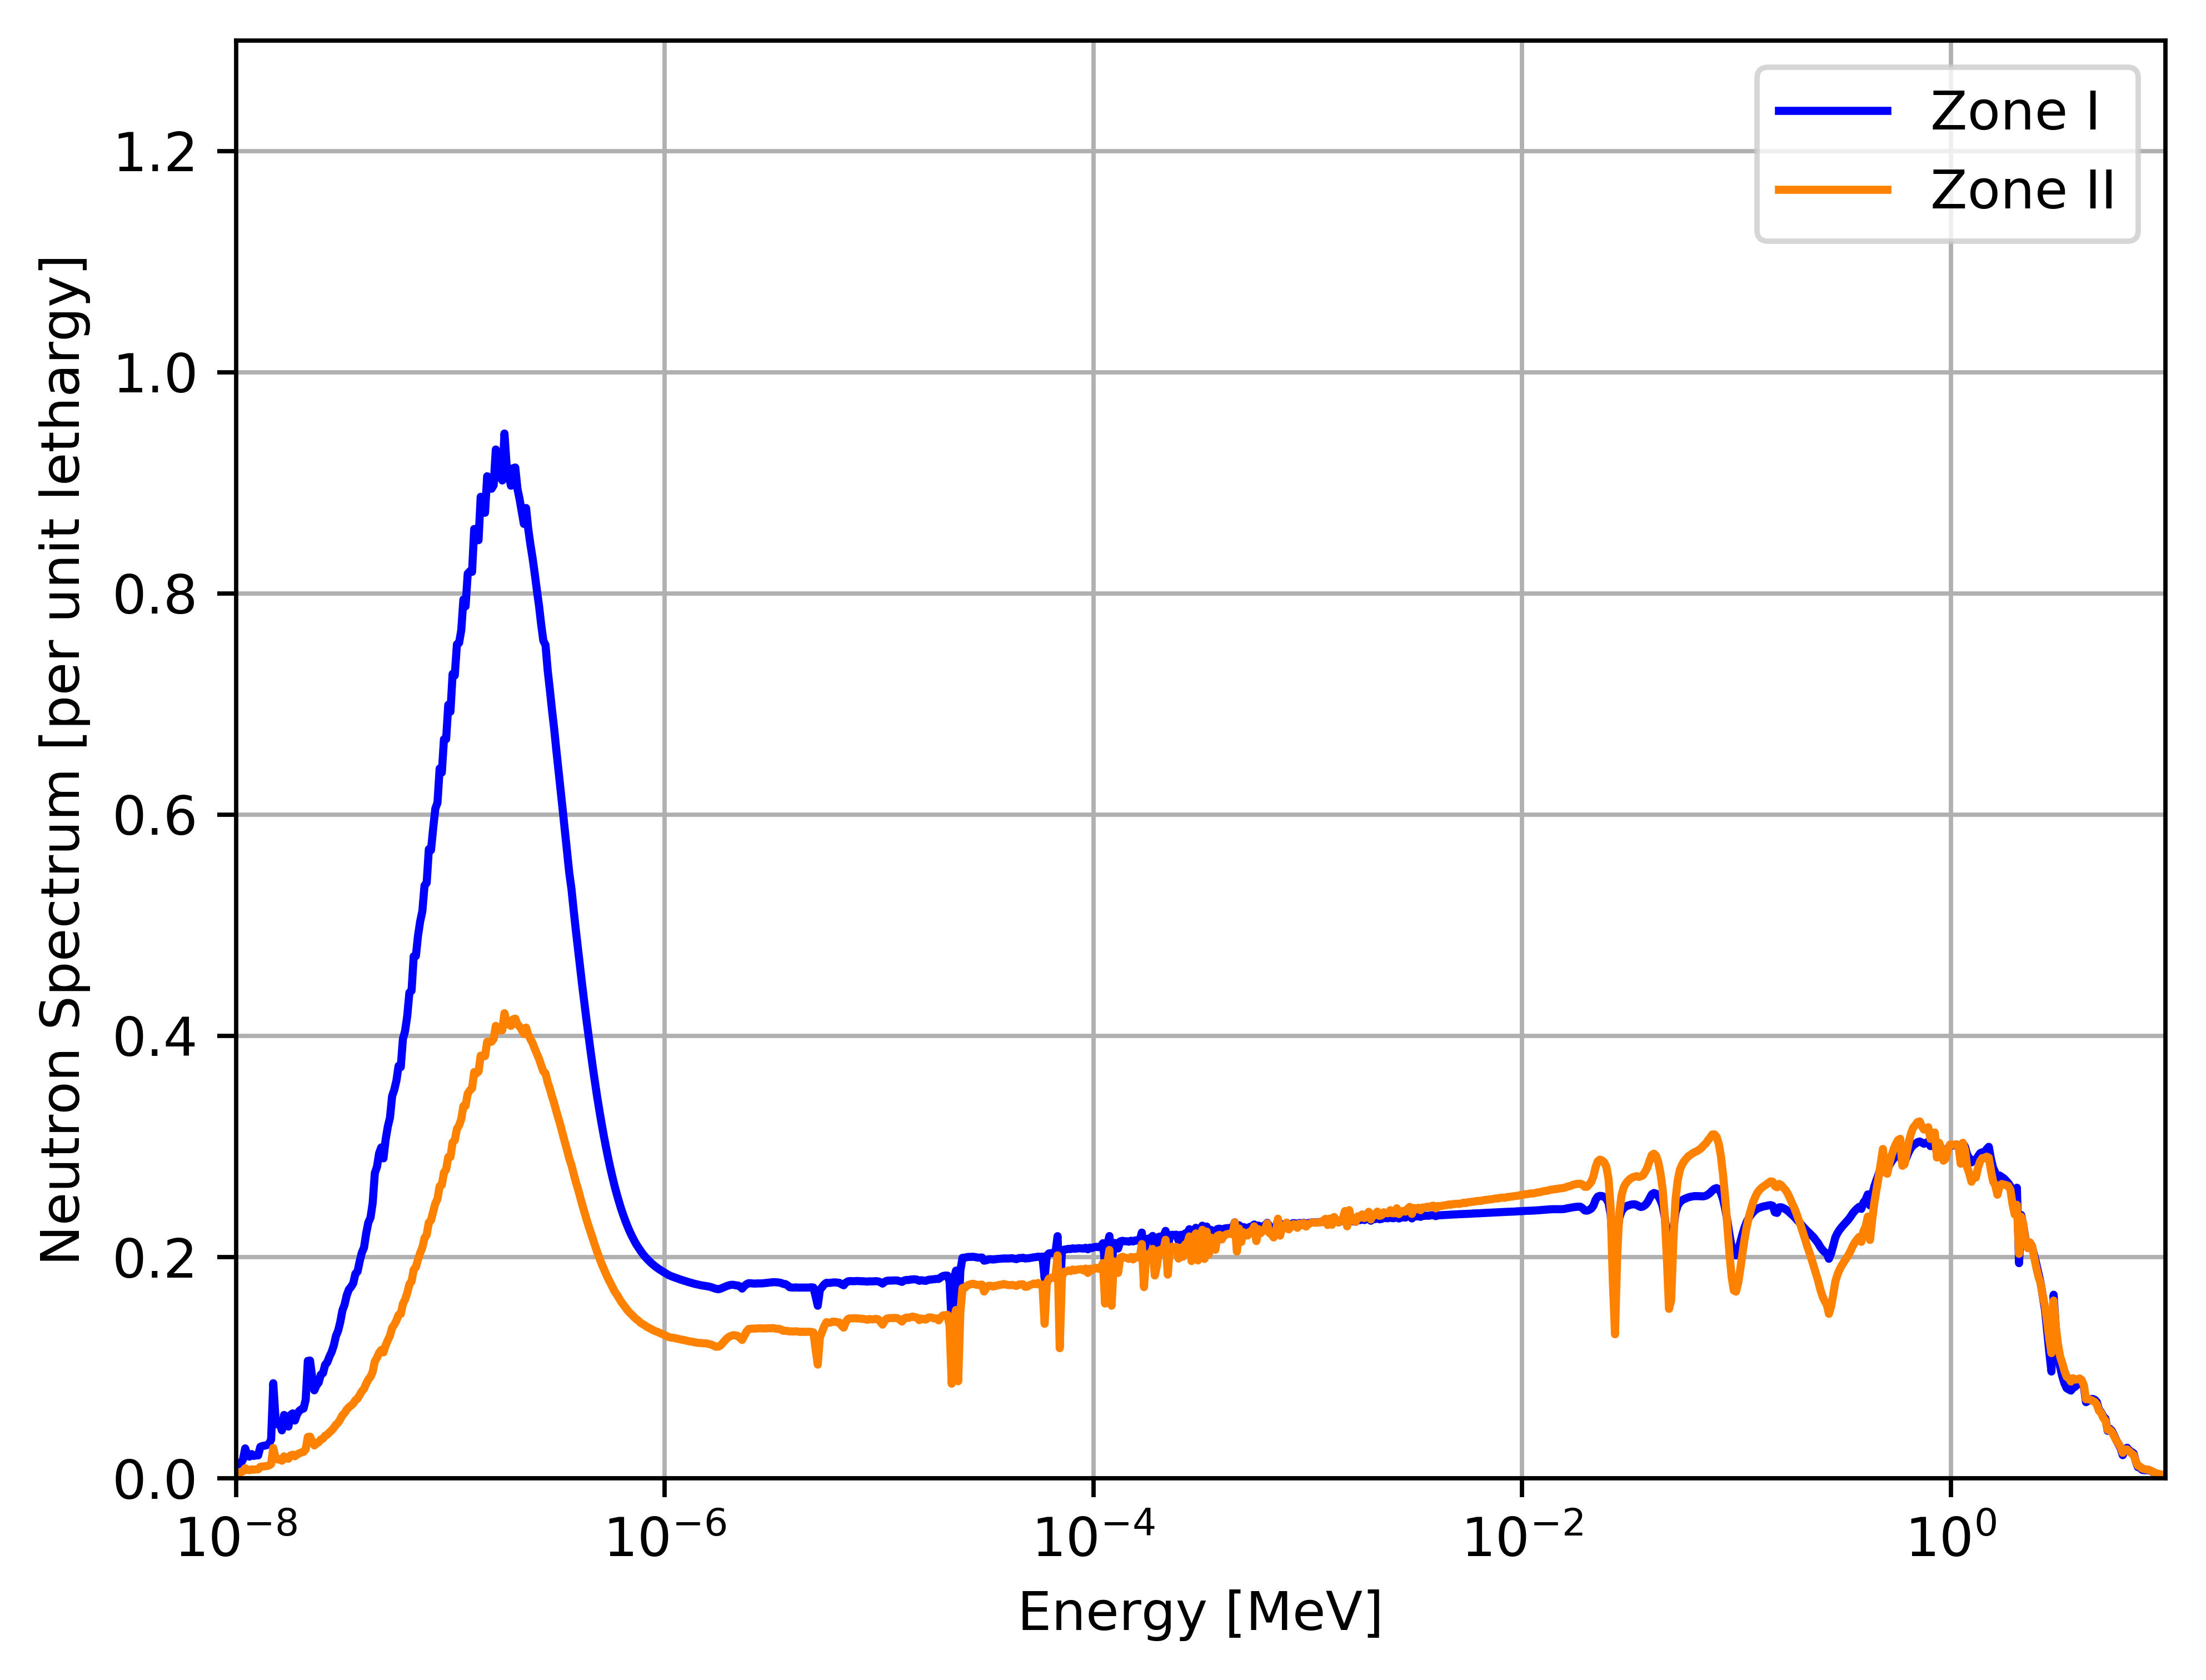
\includegraphics[width=\textwidth]{spectrum_zones_eq.png} 
      \vspace{-0.3em}
  \caption{Neutron flux energy spectrum in different core regions normalized by unit lethargy for the equilibrium fuel salt composition.}
    \vspace{-1.0em}
  \label{fig:spectrum_zones_eq}
\end{figure}
\FloatBarrier

\section{Neutron flux}
Figure~\ref{fig:radial_flux} shows the radial distribution of fast and thermal neutron flux for both initial and equilibrium composition. The neutron flux has the same shape for both compositions but the equilibrium case has a harder spectrum. A significant spectral shift was observed for the central region of the core (zone I) when for the outer region (zone II) it is negligible for fast but notable for thermal neutrons. This neutron flux radial distribution is in a good agreement with original ORNL report \cite{robertson_conceptual_1971}. Overall, spectrum hardening during \gls{MSBR} operation should be carefully studied for designing the reactivity control system.

\begin{figure}[htp!] % replace 't' with 'b' to force it to 
  \centering
    \vspace{-0.3em}
  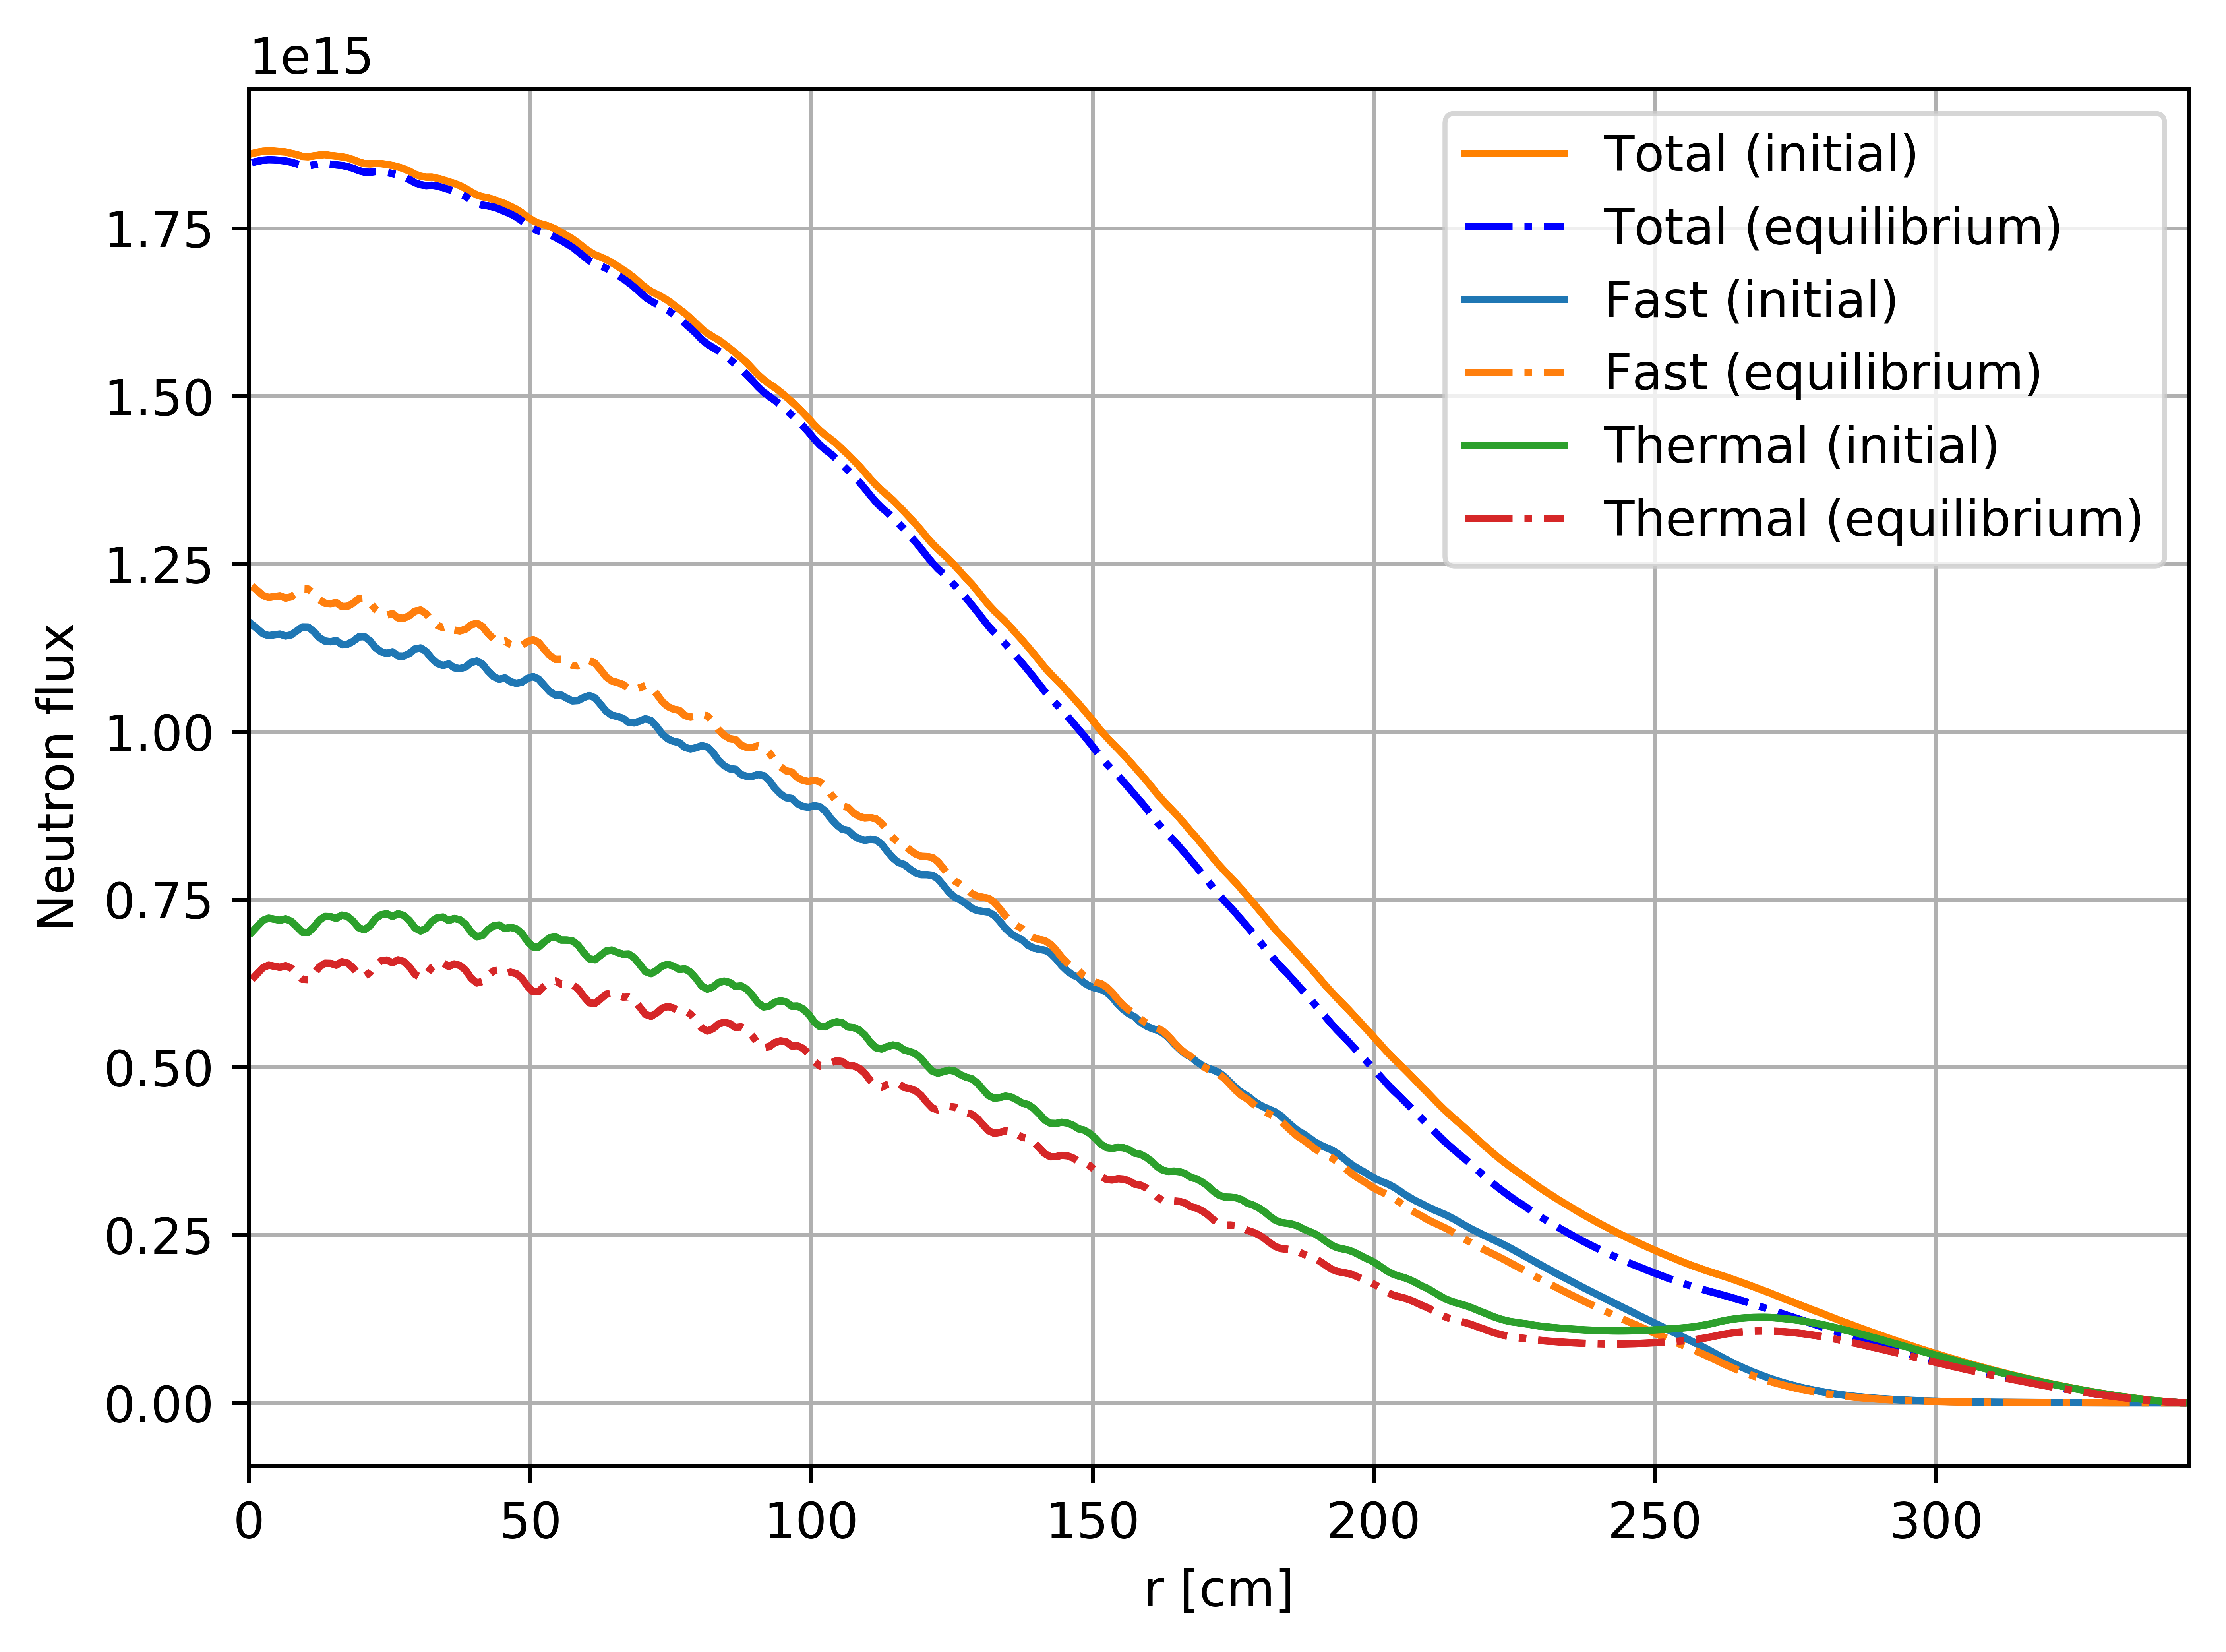
\includegraphics[width=\textwidth]{radial_flux.png} 
  \caption{Radial neutron flux distribution for initial and equilibrium fuel salt composition.}
    \vspace{-0.6em}
  \label{fig:radial_flux}
\end{figure}
\FloatBarrier

\section{Power and breeding distribution}
Table~\ref{tab:powgen_fraction} shows the power fraction in each zone for initial and equilibrium fuel composition. Figure~\ref{fig:pow_den} demonstrates the normalized power distribution of the \gls{MSBR} quater core at both states. For both the initial and equilibrium compositions, fission primarly occurs in the center of the core, namely zone I. The spectral shift during reactor operation results in different power fractions at startup and equilibrium, but most of the power is still generated in zone I. Figure~\ref{fig:breeding_den} shows the neutron capture reaction rate distribution for $^{232}$Th normalized by the total neutron flux for initial and equilibrium states. The distribution reflects the spatial distribution of $^{233}$Th production in the core. The thorium-232 then $\beta$-decays to $^{233}$Pa which is the precursor for $^{233}$U production. Accordingly, this characteristic represents the breeding distribution in the \gls{MSBR} core. Spectral shift does not cause significant changes in power nor in breeding distribution. Even after 20 years of operation, most of the power still is generated in zone I though the majority of $^{233}$Th is produced in zone II, which is in a good agreement with original ORNL report \cite{robertson_conceptual_1971}.

%%%%%%%%%%%%%%%%%%%%%%%%%%%%%%%%%%%%%%%%
\begin{table}[ht!]
  \centering
  \caption{Power generation fraction in each zone for initial and equilibrium state.}
\begin{tabular}{| m{0.22\textwidth} | m{0.22\textwidth} | m{0.22\textwidth} |} \hline
Core region      & Initial      & Equilibrium   \\ [3pt]\hline   
Zone I           & 97.91\%      & 98.12\%   \\ [3pt] \hline
Zone II          & 2.09\%       & 1.88\%   \\ [3pt] \hline
\end{tabular}
  \label{tab:powgen_fraction}
\end{table}
%%%%%%%%%%%%%%%%%%%%%%%%%%%%%%%%%%%%%%%%%%%%%%%%%%%%%%%%%%%%%%%%%%%%%%%%%%%%%%%%

\begin{figure}[htp!] % replace 't' with 'b' to force it to 
  \centering
    \vspace{-0.3em}
  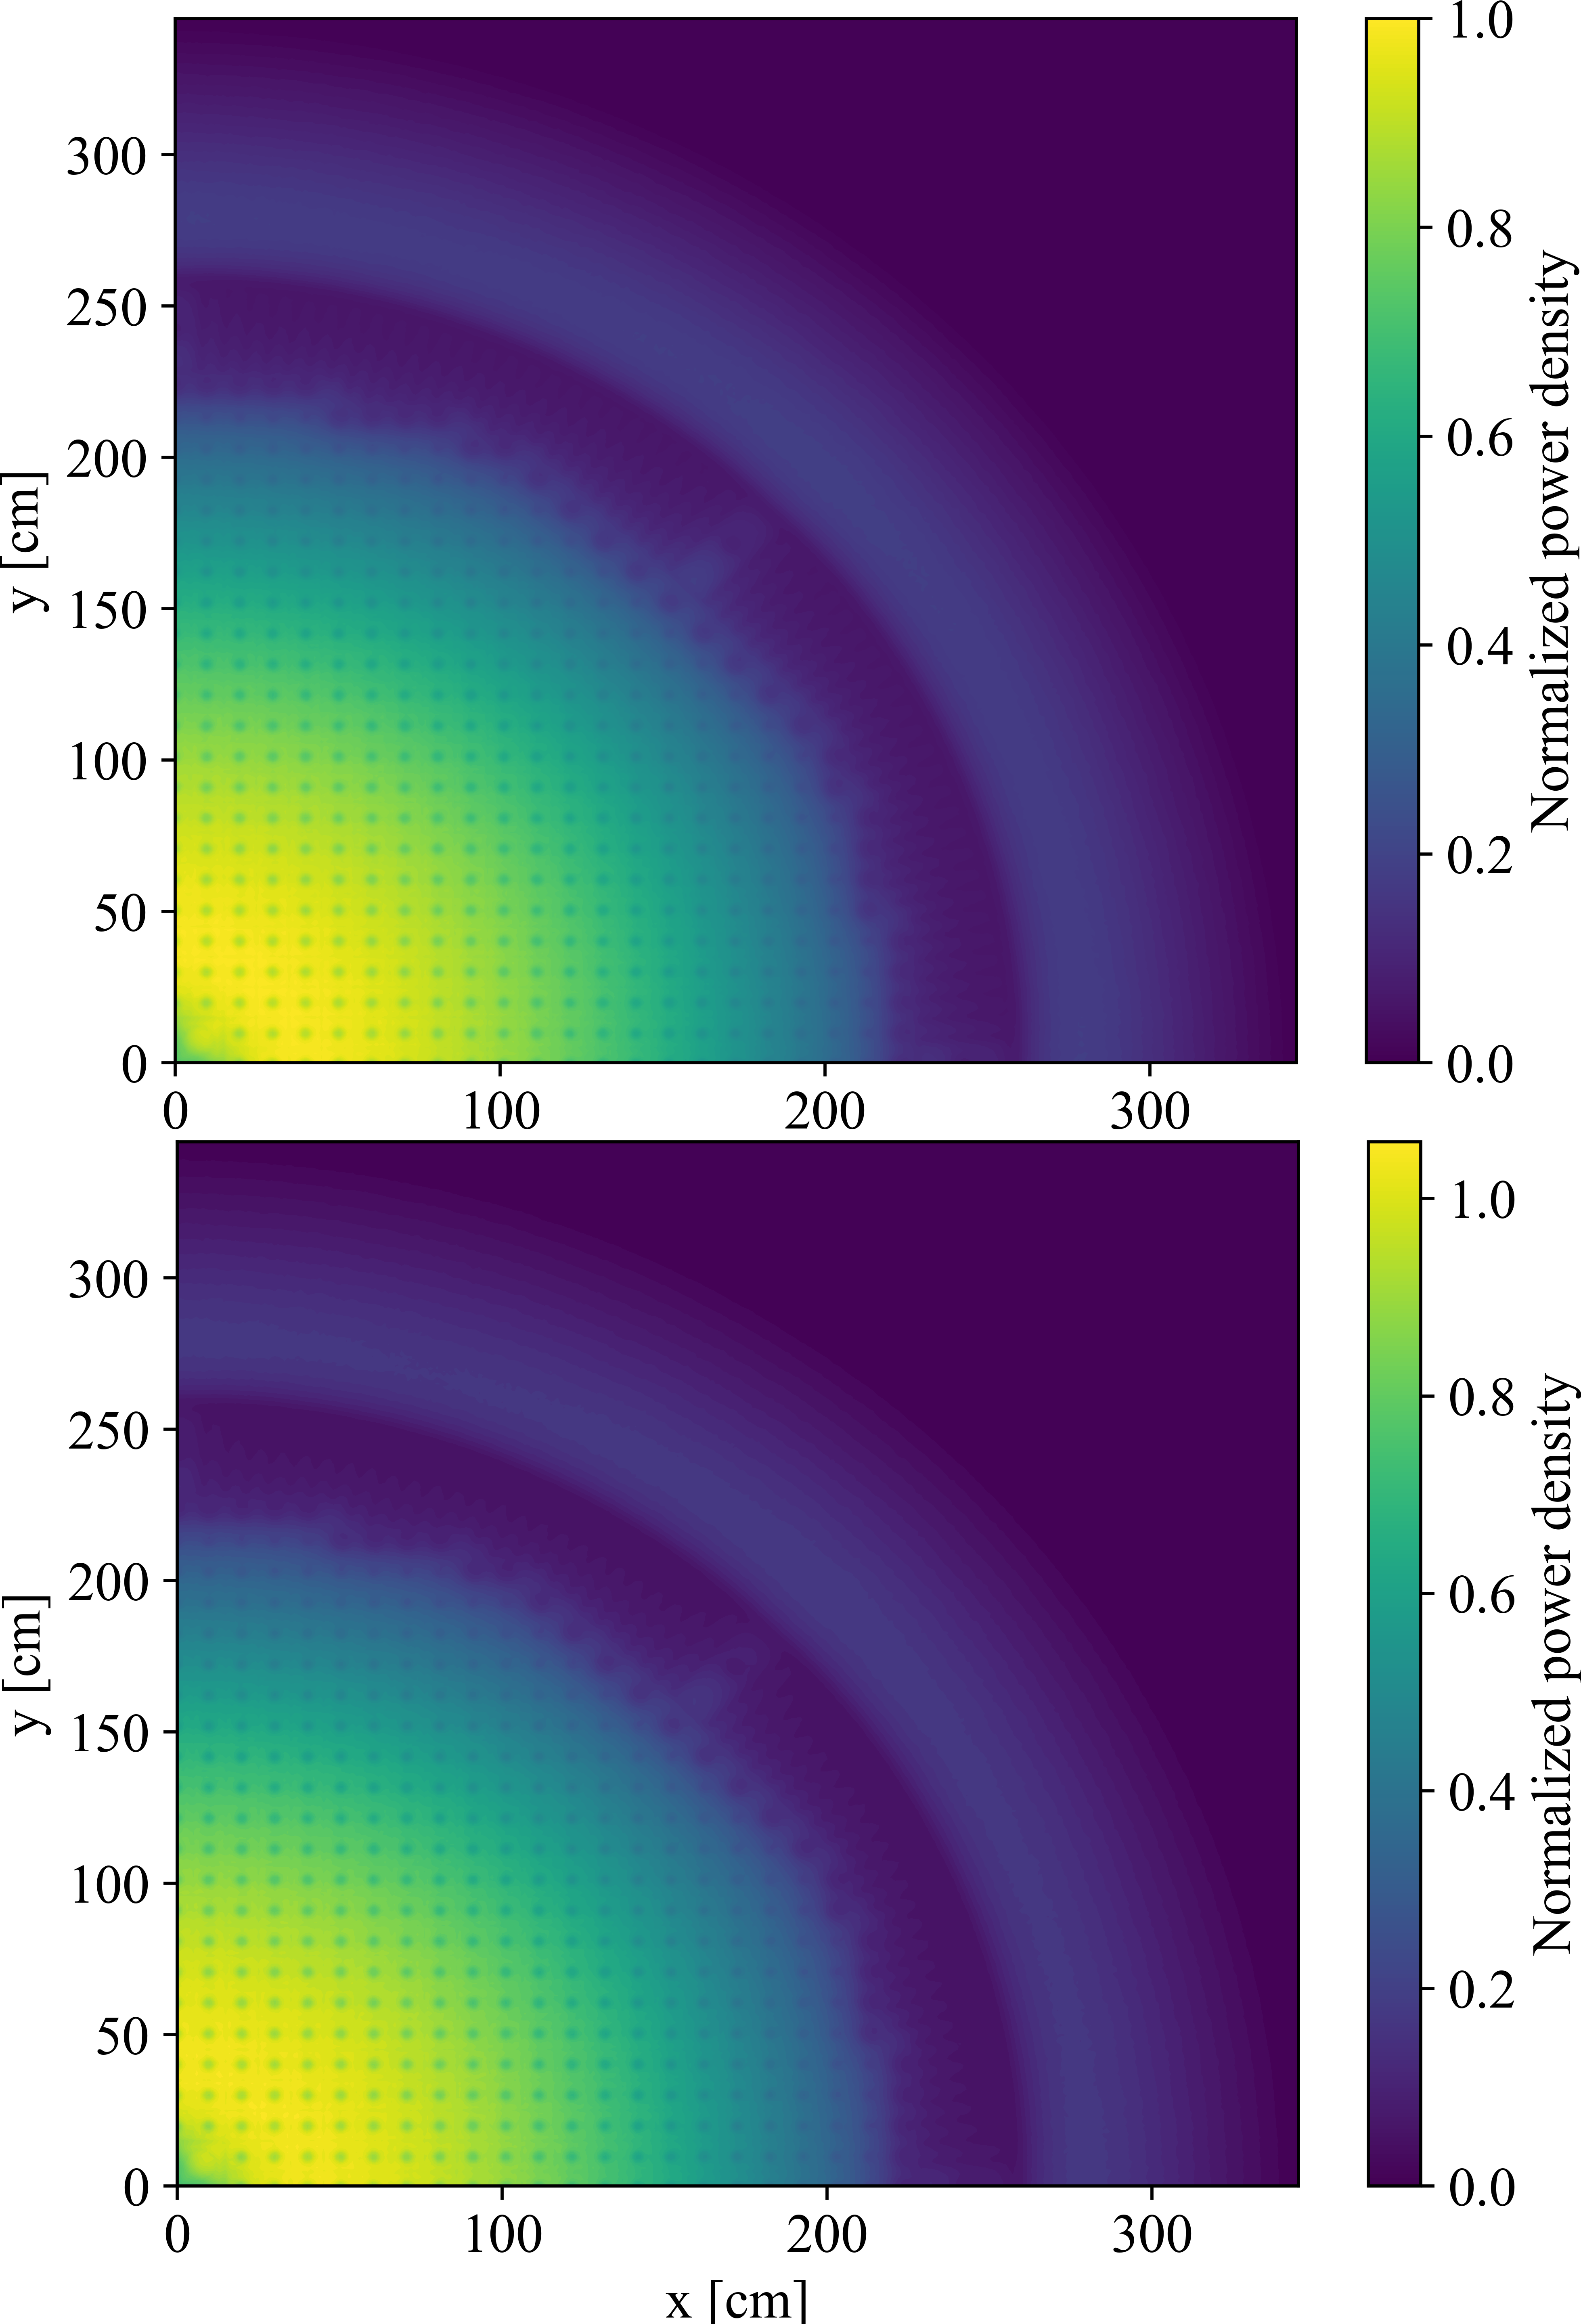
\includegraphics[width=\textwidth]{power_distribution.png} 
  \caption{Normalized power density for initial (top) and equilibrium (bottom) fuel salt composition.}
    \vspace{-0.6em}
  \label{fig:pow_den}
\end{figure}
\FloatBarrier

\begin{figure}[htp!] % replace 't' with 'b' to force it to 
  \centering
    \vspace{-0.3em}
  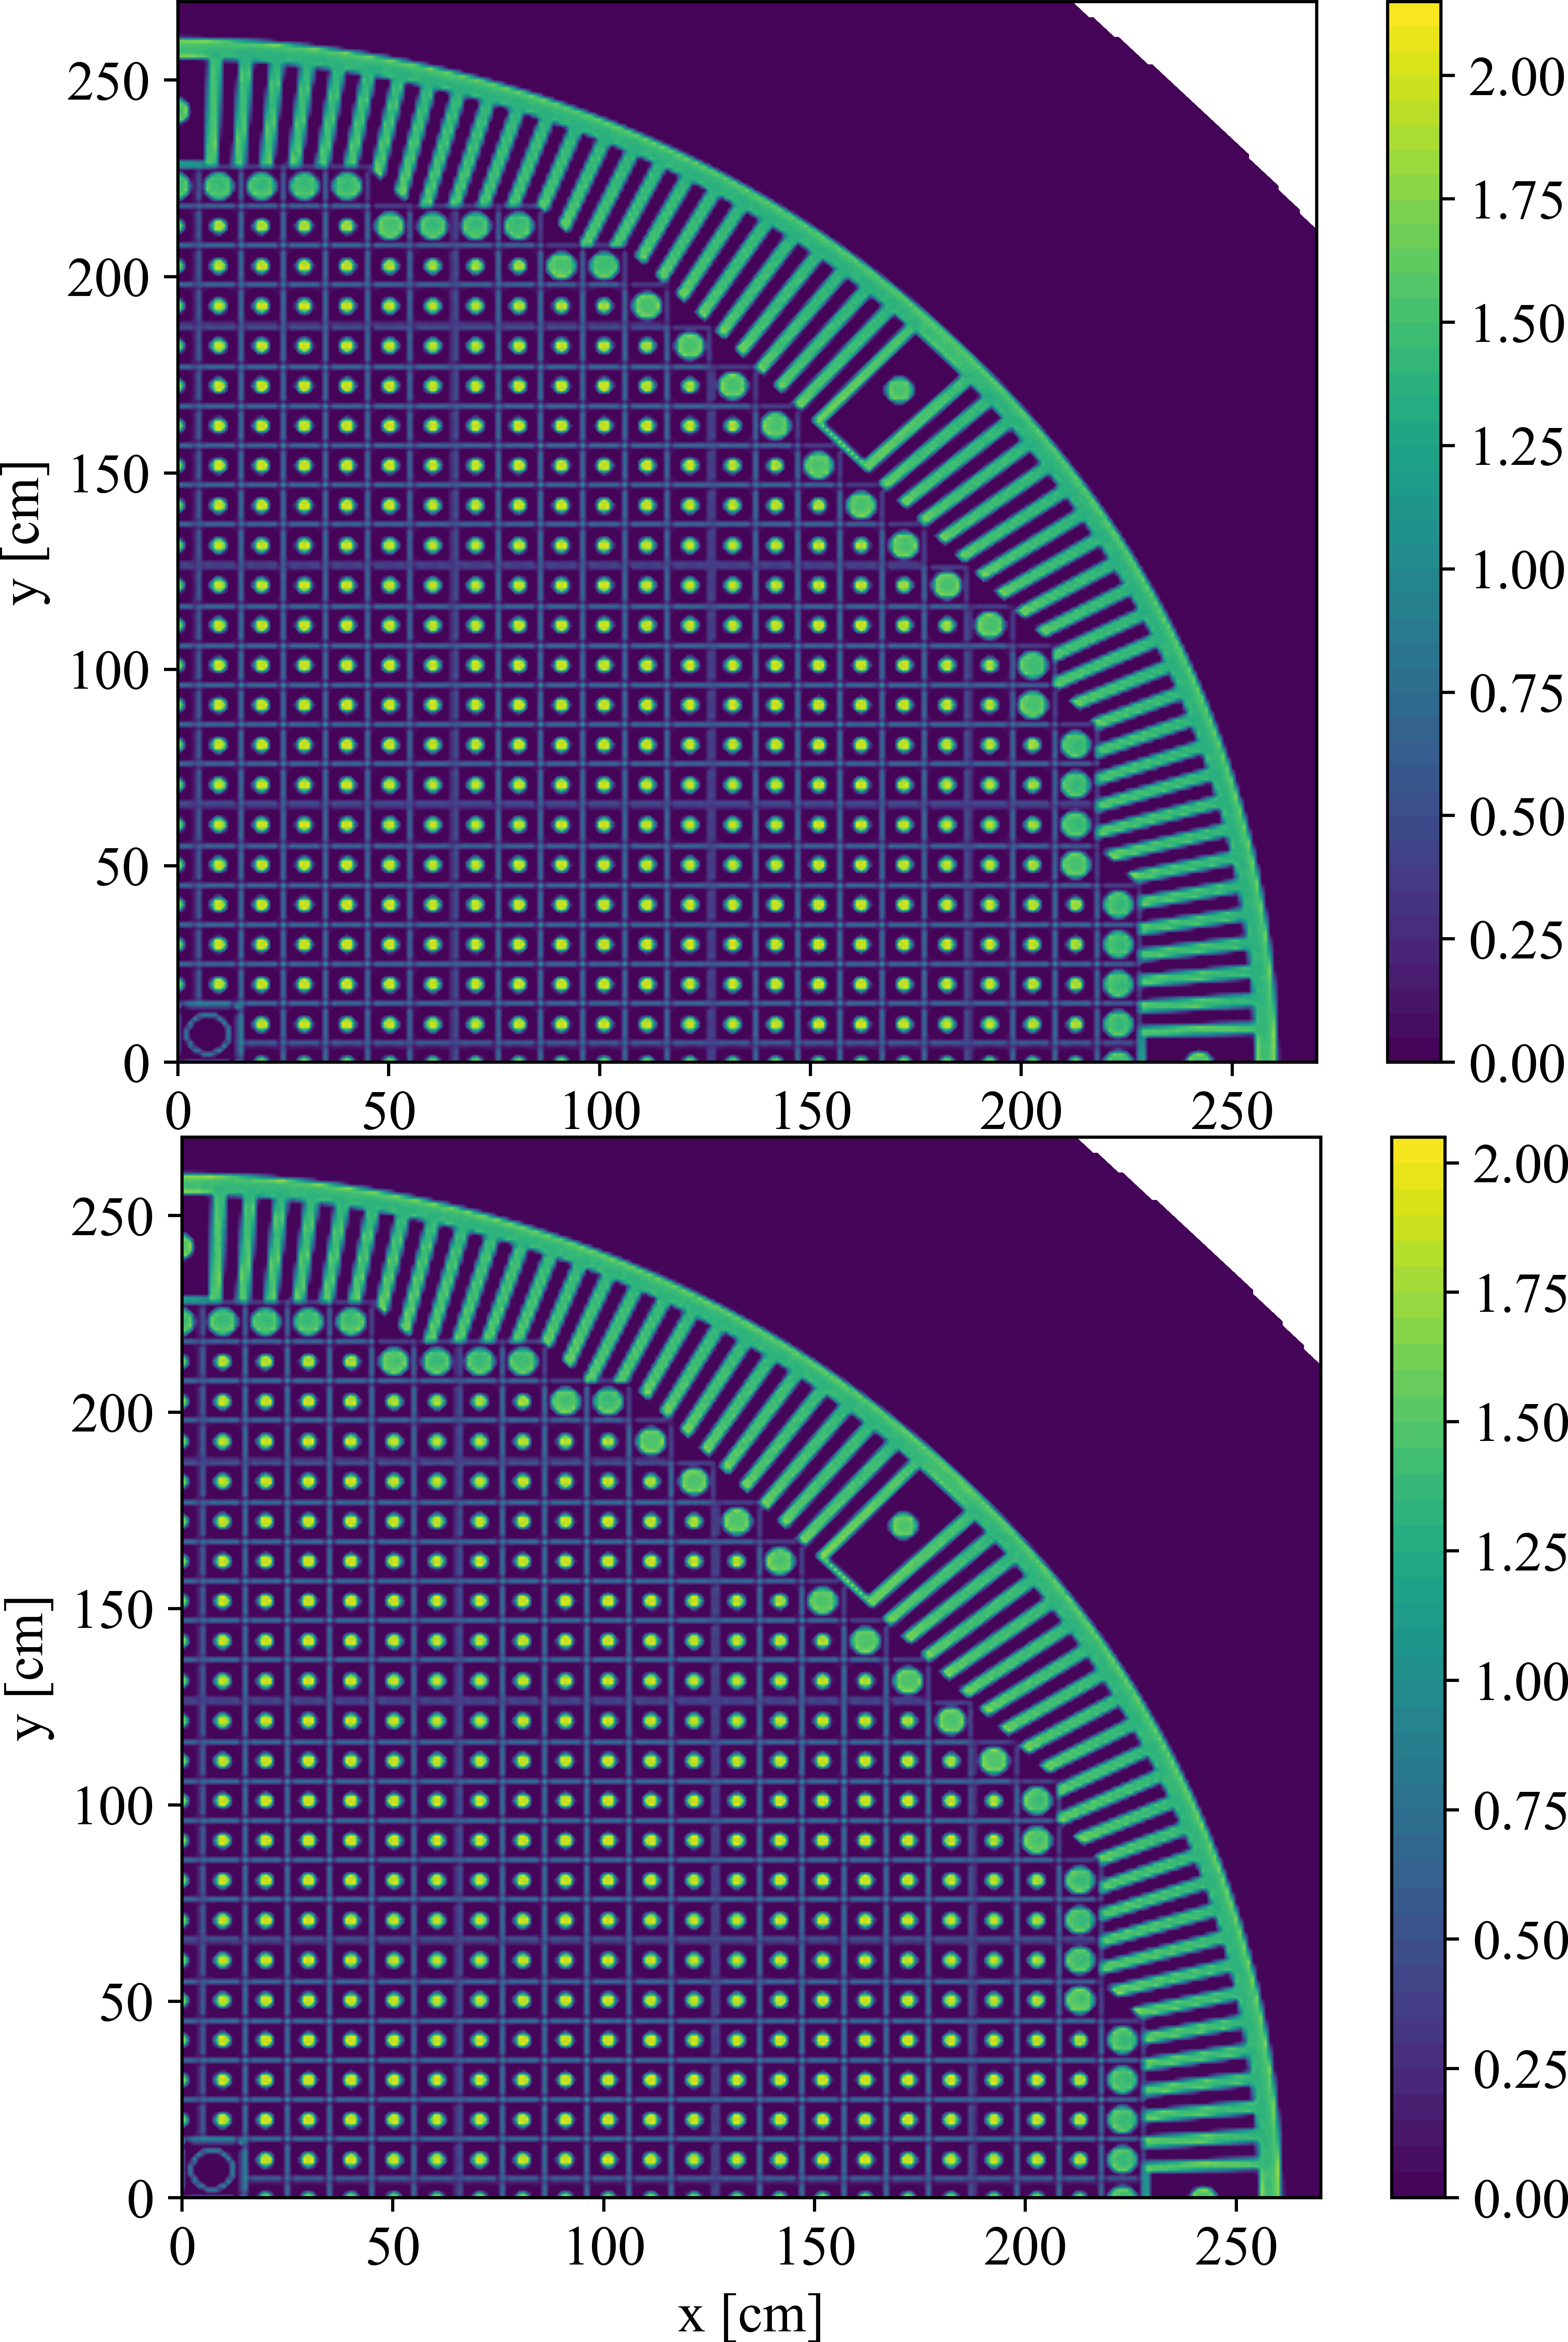
\includegraphics[width=\textwidth]{breeding_distribution.png} 
  \caption{$^{232}$Th neutron capture reaction rate normalized by total flux for initial (top) and equilibrium (bottom) fuel salt composition.}
    \vspace{-0.6em}
  \label{fig:breeding_den}
\end{figure}
\FloatBarrier

\section{Temperature coefficient of reactivity}
Table~\ref{tab:tcoef} summarizes temperature effects on reactivity calculated in this work for both initial and equilibrium fuel composition, and compared with original \gls{ORNL} report data \cite{robertson_conceptual_1971}. Uncertainty for each temperature coefficient also appears in Table~\ref{tab:tcoef}. The main physical principle underlying the reactor temperature feedback is an expansion of matterial that is heated. When the fuel salt temperature increases, the density of the salt decreases, but at the same time, the total volume of fuel salt in the core remains constant because it is bounded by the graphite. When the graphite temperature increases, the density of graphite decreases creating additional space for fuel salt. To determine temperature coefficients, the cross section temperatures for fuel and moderator were changed from 900K to 1000K. Three different cases were considered:
\begin{enumerate}
  \item Temperature of fuel salt rising from 900K to 1000K.
  \item Temperature of graphite rising from 900K to 1000K.
  \item Whole reactor temperature rising from 900K to 1000K.
\end{enumerate}

%%%%%%%%%%%%%%%%%%%%%%%%%%%%%%%%%%%%%%%%
\begin{table}[ht!]
  \centering
  \caption{Temperature coefficients of reactivity for initial and equilibrium state.}
\begin{tabular}{| m{0.22\textwidth} | m{0.22\textwidth} | m{0.22\textwidth} | m{0.20\textwidth} |} \hline
   Reactivity coefficient [pcm/K]  & Initial      & Equilibrium  & Reference \cite{robertson_conceptual_1971} \\ [5pt]\hline   
Fuel salt        & $-3.22\pm0.044$ & $-1.53\pm0.046$ & $-3.22$  \\ [3pt] \hline
Moderator        & $+1.61\pm0.044$ & $+0.97\pm0.046$ & $+2.35$  \\ [3pt] \hline
Total            & $-3.1\pm0.04$   & $-0.97\pm0.046$ & $-0.87$  \\ [3pt] \hline
\end{tabular}
  \label{tab:tcoef}
\end{table}
%%%%%%%%%%%%%%%%%%%%%%%%%%%%%%%%%%%%%%%%%%%%%%%%%%%%%%%%%%%%%%%%%%%%%%%%%%%%%%%%
In the first case, changes in the fuel temperature only impact fuel density. In this case, the geometry is unchanged because the fuel is a liquid. However, when the moderator heats up, both the density and the geometry change due to thermal expansion of the solid graphite blocks and reflector. Accordingly, the new graphite density was calculated using a linear temperature expansion coefficient of 1.3$\times10^{-6}$1/K \cite{robertson_conceptual_1971}. A new geometry input was created based on this information.

The fuel temperature coefficient (FTC) is negative for both initial and equilibrium fuel compositon due to thermal Doppler broadening of the resonance capture cross sections in the thorium and is in a good agreement with earlier research \cite{robertson_conceptual_1971,park_whole_2015}. The moderator temperature coefficient (MTC) is positive for startup composition and decreases during reactor operation because of spectrum hardening with fuel depletion. Finally, the total temperature coefficient of reactivity is negative for both cases, but decreases during reactor operation due to spectral shift. In summary, even after 20 years of operation the total temperature coefficient of reactivity is relatively large and negative during reactor operation, despite positive MTC, and affords excellent reactor stability and control.

\section{Reactivity control system rod worth}
Table~\ref{tab:rod_worth} summarizes the reactivity control system worth. During normal operation the control (graphite) rods are fully inserted, and the safety (B$_4$C) rods are fully withdrawn. To insert negative reactivity into the core, the graphite rods are gradually withdrawn from the core. In an accident, the safety rods would fall down into the core. The integral rod worths were calculated for various positions to separately estimate control (graphite) rod, safety (B$_4$C) rod, and the whole reactivity control system worth. Control rod integral worth is approximately 28 cents and stays almost constant during reactor operation. The safety rod integral worth decreases by  16.2\% during 20 years of operation because of neutron spectrum hardening and absorber accumulation in proximity to reactivity control system rods. This 16\% decline in control system worth should be taken into account in \gls{MSBR} accident analysis and safety justification.

%%%%%%%%%%%%%%%%%%%%%%%%%%%%%%%%%%%%%%%%
\begin{table}[hb!]
  \centering
  \caption{Control system rod worth for initial and equilibrium fuel composition.}
\begin{tabular}{| m{0.60\textwidth} | m{0.15\textwidth} | m{0.15\textwidth} |} \hline
\qquad\qquad Reactivity parameter  & \quad Initial      & \enspace Equilibrium      \\[3pt] \hline   
Control (graphite) rod integral worth (cents)               & $\ 28.2\pm0.8$     & $\ 29.0\pm0.8$ \\[3pt]  \hline 
Safety (B$_4$C) rod integral worth (cents)                  & $251.8\pm0.8$    & $211.0\pm0.8$  \\[3pt]  \hline
Total reactivity control system worth (cents)               & $505.8\pm0.7$    & $424.9\pm0.8$ \\[3pt] \hline
\end{tabular}
  \label{tab:rod_worth}
\end{table}
%%%%%%%%%%%%%%%%%%%%%%%%%%%%%%%%%%%%%%%%%%%%%%%%%%%%%%%%%%%%%%%%%%%%%%%%%%%%%%%%

\section{Six Factor Analysis}
The effective multiplication factor could be expressed using formula:
\begin{align*}
k_{eff} = k_{inf} P_f  P_t \\
 = \eta \epsilon p f P_f P_t
\end{align*}

%%%%%%%%%%%%%%%%%%%%%%%%%%%%%%%%%%%%%%%%
\begin{table}[ht!]
  \centering
  \caption{Six factors for the full-core \gls{MSBR} model for initial and equilibrium fuel composition.}
\begin{tabular}{| m{0.44\textwidth} | m{0.22\textwidth} | m{0.22\textwidth} |} \hline
	   \qquad\qquad\qquad Factors  & \qquad Initial      & \qquad Equilibrium   \\ [3pt]\hline   
Neutron reproduction factor ($\eta$)     & $1.3960\pm.000052$     & $1.3778\pm.00005$ \\ [3pt] \hline
Thermal utilization factor (f)           & $0.9670\pm.000011$     & $0.9706\pm.00001$ \\ [3pt] \hline
Resonance escape probability (p)         & $0.6044\pm.000039$     & $0.5761\pm.00004$ \\ [3pt] \hline
Fast fission factor ($\epsilon$)         & $1.3421\pm.000040$     & $1.3609\pm.00004$ \\ [3pt] \hline
Fast non-leakage probability (P$_f$)     & $0.9999\pm.000004$     & $0.9999\pm.000004$ \\ [3pt] \hline
Thermal non-leakage probability (P$_t$)  & $0.9894\pm.000005$     & $0.9912\pm.00005$ \\ [3pt] \hline
\end{tabular}
  \label{tab:six_factor}
\end{table}
%%%%%%%%%%%%%%%%%%%%%%%%%%%%%%%%%%%%%%%%%%%%%%%%%%%%%%%%%%%%%%%%%%%%%%%%%%%%%%%%

Table~\ref{tab:six_factor} summarizes the six factors for both initial and equilibrium fuel salt composition. The non-leakage probability for both fast and thermal neutrons does not change during reactor operation because these values are not largely affected by the neutron spectrum shift. In contrast, neutron reproduction factor ($\eta$), resonance escape probability (p), and fast fission factor ($\epsilon$) are considerably different between startup and equilibrium. As indicated in Figure~\ref{fig:spectrum} the neutron spectrum is softer for the initial state. Neutron spectrum hardening causes the fast fission to increase throught the core lifetime. The opposite is true for the resonance escape probability. Finally, the neutron reproduction factor decreases during reactor operation due to accumulation of fissile plutonium isotopes.

\section{Thorium refill rate}
As was mentioned in Chapter 4, the only external feed material flow for this \gls{MSBR} reprocessing scheme is $^{232}$Th. Figure~\ref{fig:th_refill} shows the $^{232}$Th feed rate calculated for 20 years of reactor operation. Figure~\ref{fig:th_refill_spike} shows the large spikes up to 36 kg/day in a thorium consumption every 3435 days. This is required due to batch-wise removal of strong absorbers (Rb, Sr, Cs, Ba). The corresponding effective multiplication factor increase (Figure~\ref{fig:keff}) and breeding intensification leads to additional $^{232}$Th consumption. As indicated in Figure~\ref{fig:th_refill}, the average thorium feed rate increases during the first 500 days of operation and than steadily decreases due to spectrum hardening and accumulation of absorbers in the core. As a result, the average $^{232}$Th feed rate over 20 years of operation is about 2.39 kg/day. This results is in a good agreement with a recent online reprocessing study by \gls{ORNL} \cite{betzler_molten_2017} which reported thorium-232 refill rate for single-cell online reprocessing of 2.45 kg/day.

\begin{figure}[htp!] % replace 't' with 'b' to force it to 
  \centering
    \vspace{-0.3em}
  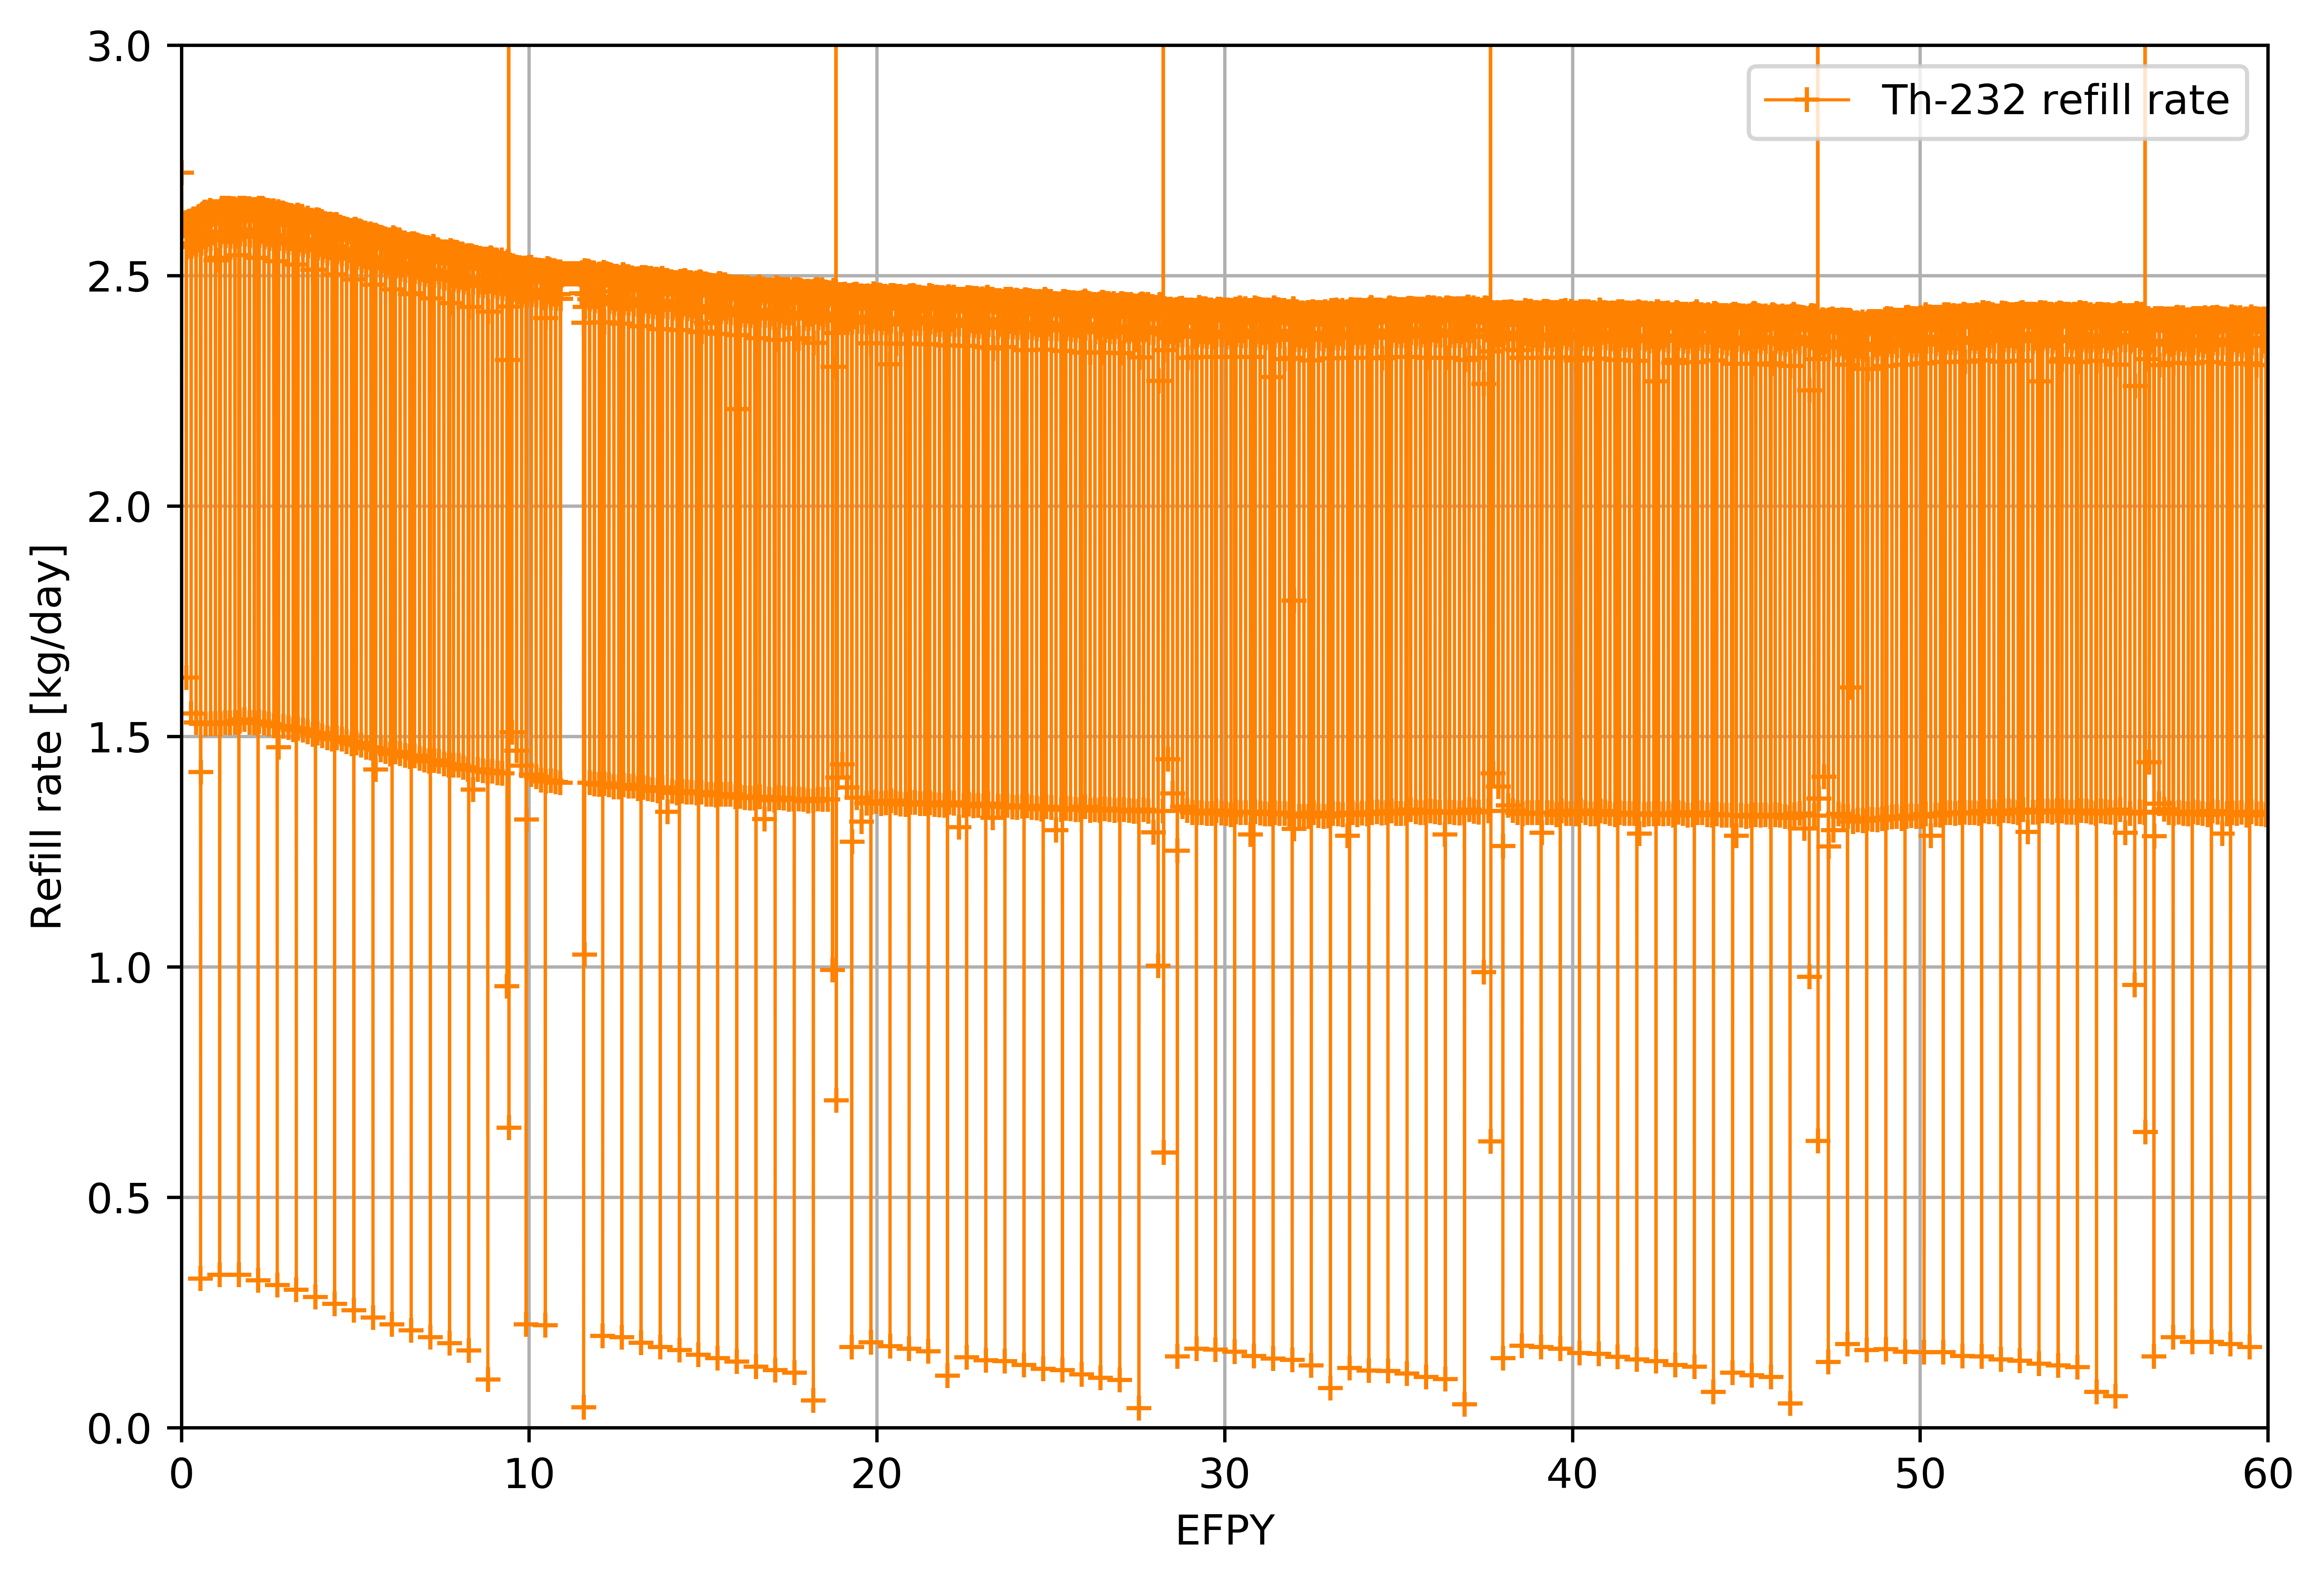
\includegraphics[width=\textwidth]{Th_refill_rate.png} 
      \vspace{-1.5em}
  \caption{$^{232}$Th feed rate over 20 years of \gls{MSBR} operation.}
    \vspace{-0.6em}
  \label{fig:th_refill}
\end{figure}
\begin{figure}[htp!] % replace 't' with 'b' to force it to 
  \centering
    \vspace{-0.3em}
  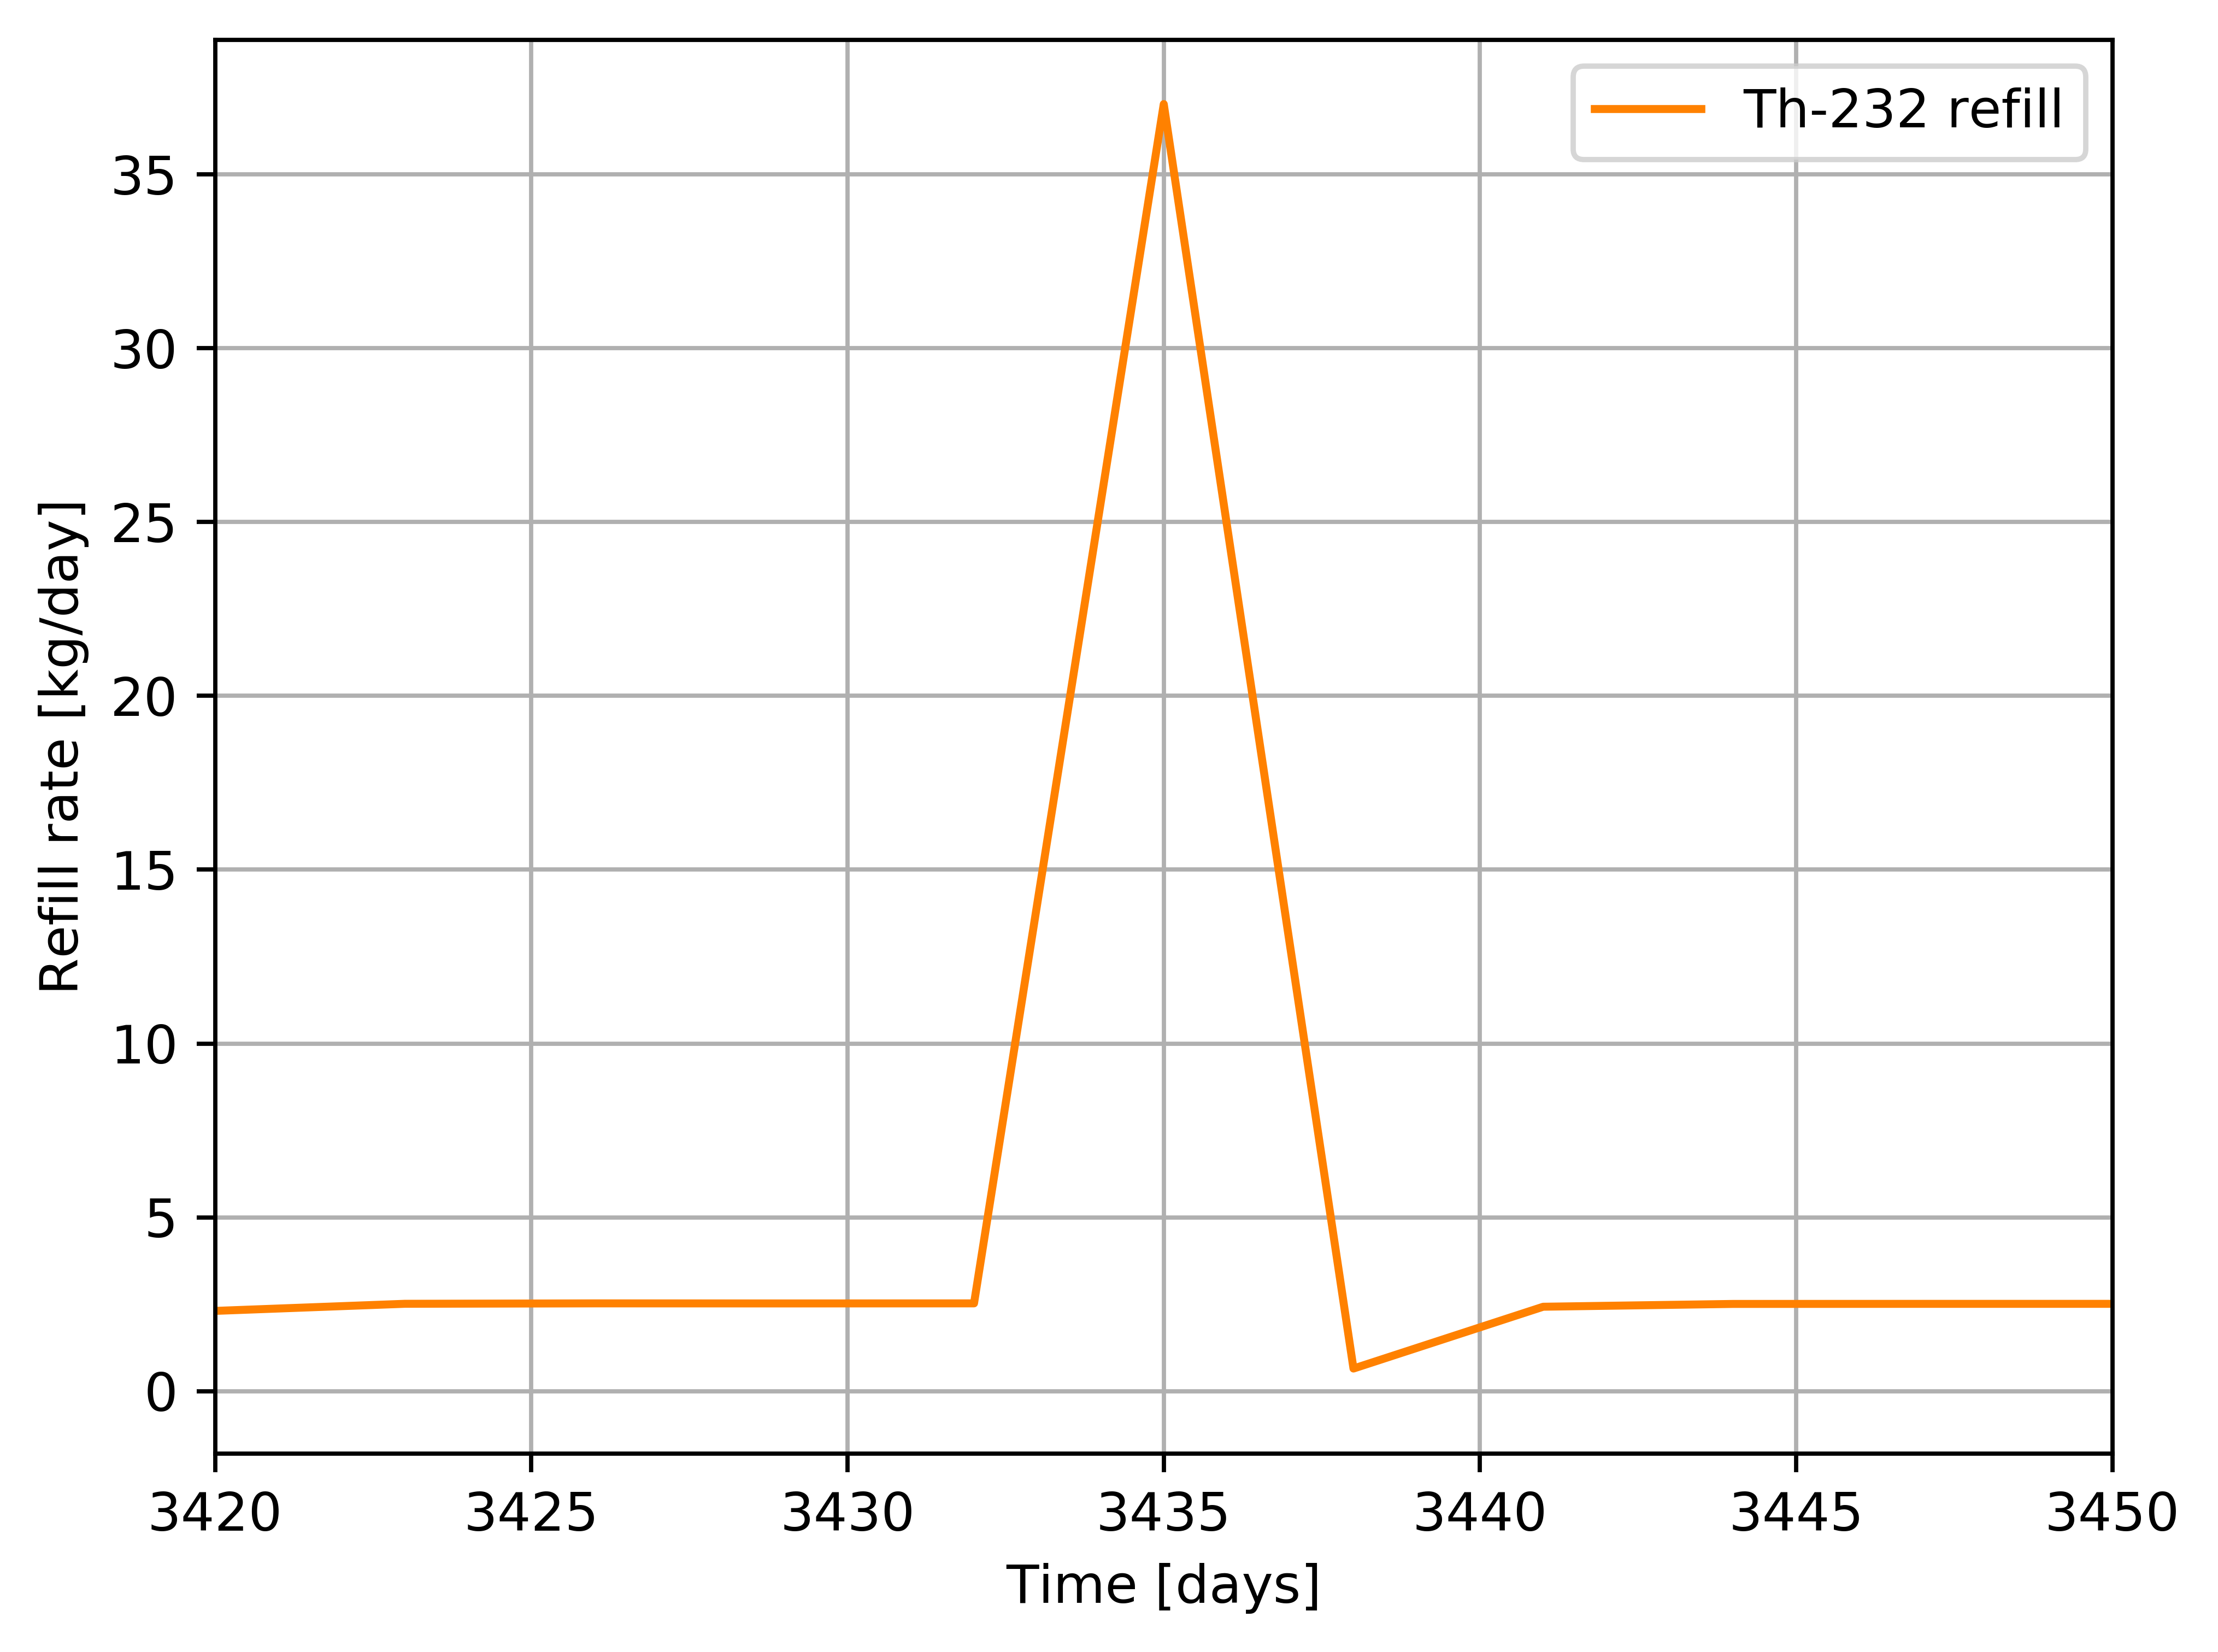
\includegraphics[width=\textwidth]{Th_refill_rate_spike.png} 
      \vspace{-1.5em}
  \caption{Typical $^{232}$Th feed rate spike caused by strong absorbers (Rb, Sr, Cs, Ba) removal.}
    \vspace{-0.6em}
  \label{fig:th_refill_spike}
\end{figure}
\FloatBarrier

\chapter[Future work and Proposed simulations]{Future work and Proposed 
simulations}

\section{Summary}
The need for this work has been shown by a summary of the current state of the 
art of \gls{MSR} depletion simulator capabilities. The literature review in 
Chapter 1 concluded that most \gls{MSR} depletion simulators typically assume 
ideal (rather than realistically constrained) poison removal rates for the 
nuclear system performance modeling. Moreover, most of the simulators assumed 
constant extraction efficiency vectors, which must be determined by the user 
in the input file and cannot be a function of other parameters. The Python 
toolkit, SaltProc v1.0, will directly couple with the Serpent 2 Monte Carlo 
depletion code for liquid-fueled \gls{MSR} depletion simulation to enable 
realistic online reprocessing system modeling. The SaltProc v1.0 seeks to be a 
universal tool for fuel composition evolution analysis in \glspl{MSR} with 
taking into account the complex fuel salt reprocessing system. Such 
reprocessing systems may consist of multiple components with variable removal 
efficiencies and rates. Moreover, these components can be connected in series, 
parallel, or a combination, which will be accurately treated in the SaltProc 
v1.0. Section~\ref{sec:reproc-plant} details the generic design of \gls{MSR}  
fuel salt reprocessing systems. Section~\ref{sec:tool_design} describes the  
SaltProc v1.0 architecture and design that is required to successfully model 
comprehensive liquid-fueled \glspl{MSR} with online fuel reprocessing systems. 

Figure~\ref{fig:workflow} shows an outline of this work. The current chapter 
details each Stage of the proposed work.
 \begin{sidewaysfigure}[ht!] % replace 't' with 'b' to force it to 
 	\centering
 	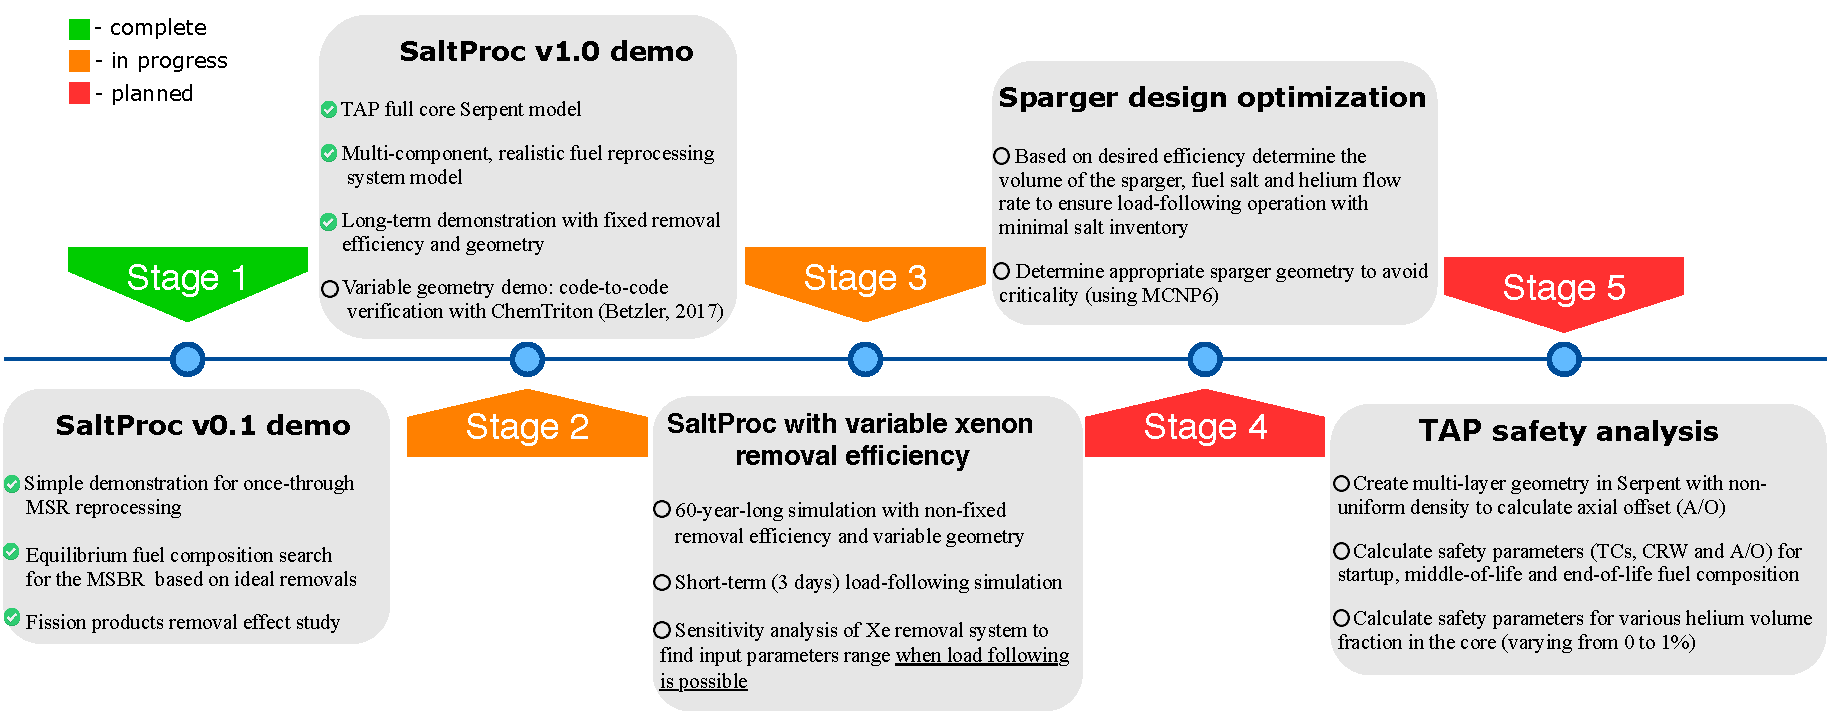
\includegraphics[width=1.06\textwidth]{progress_chart.pdf} 
 	\caption{Workflow for the simulations proposed in this work.}
 	\label{fig:workflow}
 \end{sidewaysfigure}
 \FloatBarrier
 
 
\section{Stage 1: Basic online reprocessing demonstration}
In Stage 1, \gls{MSR} online reprocessing simulation capabilities have been 
reviewed and summarized (Chapter 1). SaltProc v0.1 was demonstrated for 
simplified burnup calculation for the \gls{MSBR} as a part of my M.Sc. thesis  
\cite{rykhlevskii_advanced_2018} and published paper  
\cite{rykhlevskii_modeling_2019}. These efforts illuminated depletion of the 
fuel salt in the \gls{MSBR} for 60 years of operation and took into account 
the following processes:
\begin{enumerate}
	\item \gls{FP} removal from the salt with fixed, ideal extraction 
	efficiencies (the fuel reprocessing system removed 100\% of target 
	poisons).
	\item $^{233}$Pa removal (100\%) and feed of an equal mass of $^{233}$U 
	into the core (instantaneous $^{233}$Pa decay to $^{233}$U was assumed).
	\item Fresh fertile material ($^{232}$Th) feed to maintain the constant 
	fuel salt inventory.
\end{enumerate}
Additionally, the effect of removing fission products from the fuel salt was 
investigated separately for a different group of \glspl{FP} (noble gases, 
noble and seminoble metals, rare earth elements). As expected, removing  
fission products provides significant neutronic benefit and enables a longer 
core lifetime. Section~\ref{sec:pre-results-msbr} described key findings after 
completing Stage 1.

\section{Stage 2: SaltProc v1.0 demonstration and validation for the TAP}
Simulating a realistic multi-component fuel reprocessing system is important 
for calculating an accurate fuel salt composition. SaltProc v0.1 was 
completely refactored for modeling a complicated salt reprocessing system. To 
demonstrate SaltProc v1.0 capabilities, we have created a full-core \gls{TAP} 
\gls{MSR} model in Serpent 2 \cite{chaube_tap_2019} which was described in 
detail in Section~\ref{sec:tap_model}. Moreover, the multi-component fuel 
reprocessing system of the \gls{TAP} was developed on this stage 
(Section~\ref{sec:stage2-demo}). Section~\ref{sec:stage2-demo} also presented 
preliminary results of Stage 2. The Stage 2 demonstration case has following 
advantages over Stage 1:
\begin{itemize}
	\item SaltProc v0.1 (Stage 1) approximated the fuel salt reprocessing 
	system 
	as a single ``black'' box, which removes the entire mass (100\% removal 
	efficiency) of processed elements at once. In contrast, SaltProc v1.0 
	treats the fuel reprocessing system as a complex structure of components, 
	each removing a specific set of elements with specific extraction 
	efficiency. 
	\item SaltProc v1.0 inherently checks mass conservation at each depletion 
	step and dynamically calculates feed stream to maintain the fuel salt 
	inventory constant.
	\item SaltProc v1.0 tracks the waste stream from each component.
\end{itemize}

The foremost future effort in this stage is to enable switching between 
multiple Serpent geometries during simulation. For the \gls{TAP} concept, the 
number of moderator rods in the core varies from 1332 at the startup to 6700 
at the \gls{EOL}. The user will have an option to choose when SaltProc v1.0 
should switch to next geometry: (1) after a specific depletion  time (e.g., 18 
months which is a common maintenance/refueling shutdown interval for 
\glspl{LWR}); or (2) when the effective multiplication factor reaches a 
specific value (e.g., $1.00<k_{eff} < 1.002$). Additionally, SaltProc v1.0 
will correct the total fuel salt inventory in the primary loop to compensate 
for the core geometry change. Overall, the adjustable geometry capability will 
realistically simulate long-term (60 year) operation of the \gls{TAP} reactor 
to obtain accurate fuel salt composition at different moments during operation.

Results obtained in Stage 2 will be used for code-to-code verification with  
ChemTriton/Shift results for full-core \gls{TAP} core geometry from the most 
recent \gls{ORNL} technical report TM-2017/475 \cite{betzler_assessment_2017}. 
Notably, the fuel salt composition evolution during the \gls{TAP} reactor 
operation and corresponding core geometry are determinative for all next 
stages.

This work is developed with a test-driven development paradigm. Specifically, 
before any new functionality is implemented, a suite of tests is written, 
which as carefully define its expected behavior as possible. The code is then 
written to pass the test suite. In this way, the tool developed in this work 
is expected to be comprehensively tested in parallel with its development. 
Thus, after code-to-code verification with ChemTriton/Shift multiple-component 
integration tests will be added to the test harness to make sure that future 
changes in the code will not break previous functionality.

Test problems will help comprehensively define and confirm each unit of the 
demonstration functionality. These problems will include fundamental, 
information-passing tests as well as more challenging multiple-component 
integration tests. Every unit of functionality within the toolkit will be 
tested as an integral part of development.

This milestone will result in a processing system model capable of simulating
various liquid-fueled \glspl{MSR} with multi-component fuel reprocessing 
systems but with constant separation efficiencies, defined at runtime. 
Additionally, this stage will demonstrate a key feature of the \gls{TAP} 
\gls{MSR} - adjusting the moderator rod configuration - which is necessary to 
maintain the reactor criticality during the 60-years lifetime. 

\section{Stage 3: Variable xenon extraction rate}
When Stage 2 is complete, a series of extensions to the Stage 2 model will 
be pursued. These will incorporate extraction efficiencies as a function of 
many physical system design parameters (e.g., void fraction in the salt, 
helium bubble size). Mathematical correlations for the efficiencies will be 
taken from relationships in the literature \cite{peebles_removal_1968, 
gabbard_development_1974} and CFD simulations currently being conducted 
at the University of Illinois at Urbana-Champaign \cite{huff_enabling_2018}. 
For demonstration proposes, just xenon removal efficiency will be defined as a 
function of many parameters (Section~\ref{sec:gas-separ}) due to 
limited data provided in the listed literature. For other fission products  
from the \gls{TAP} reprocessing scheme (table~\ref{tab:reprocessing_list}), 
removal efficiencies will be defined based on the removal rates from the 
table, assuming time-independent extraction efficiency. This milestone will 
result in a realistic online reprocessing system model capable of modeling 
\gls{MSR} systems with parameterized, realistically achievable process rates,  
and extraction efficiencies.

Another anticipated extension will test the \gls{TAP} reactor ability to 
operate in a load-following regime. Short-term (3 days) depletion using 
SaltProc v1.0 will be performed with the core power changing in the [0, 100\%] 
range with a ramp rate 10\%/min (to be competitive with natural gas peaking 
plants, which ramp at or above 10\% of their capacity) 
\cite{huff_enabling_2018}. 
Figure~\ref{fig:load} shows the load curve selected to demonstrate the 
worst-case scenario of load-following:
\begin{enumerate}
	\item Startup with fresh fuel and operating on 100\% of \gls{HFP}
level 
	for 40 hours to reach $^{135}$Xe/$^{135}$I equilibrium;
	\item Load-following power drop (0.1 \gls{HFP}/min), from \gls{HFP} 
	to \gls{HZP};
	\item Shutdown for 8 hours\footnote{At startup. Time after shutdown when 
	$^{135}$Xe concentration would reach maximum value greatly depends on 
	neutron energy spectrum which for the \gls{TAP} concept changes 
	significantly during operation.} to reach the $^{135}$Xe peak;
	\item Load-following power rise (0.1 \gls{HFP}/min), from \gls{HZP} 
	to \gls{HFP}.
\end{enumerate}
This scenario can be considered as backing up solar power with
nuclear on a 
high-solar penetration grid (e.g., in California).
\begin{figure}[bth!] % replace 't' with 'b' to 
	\centering
	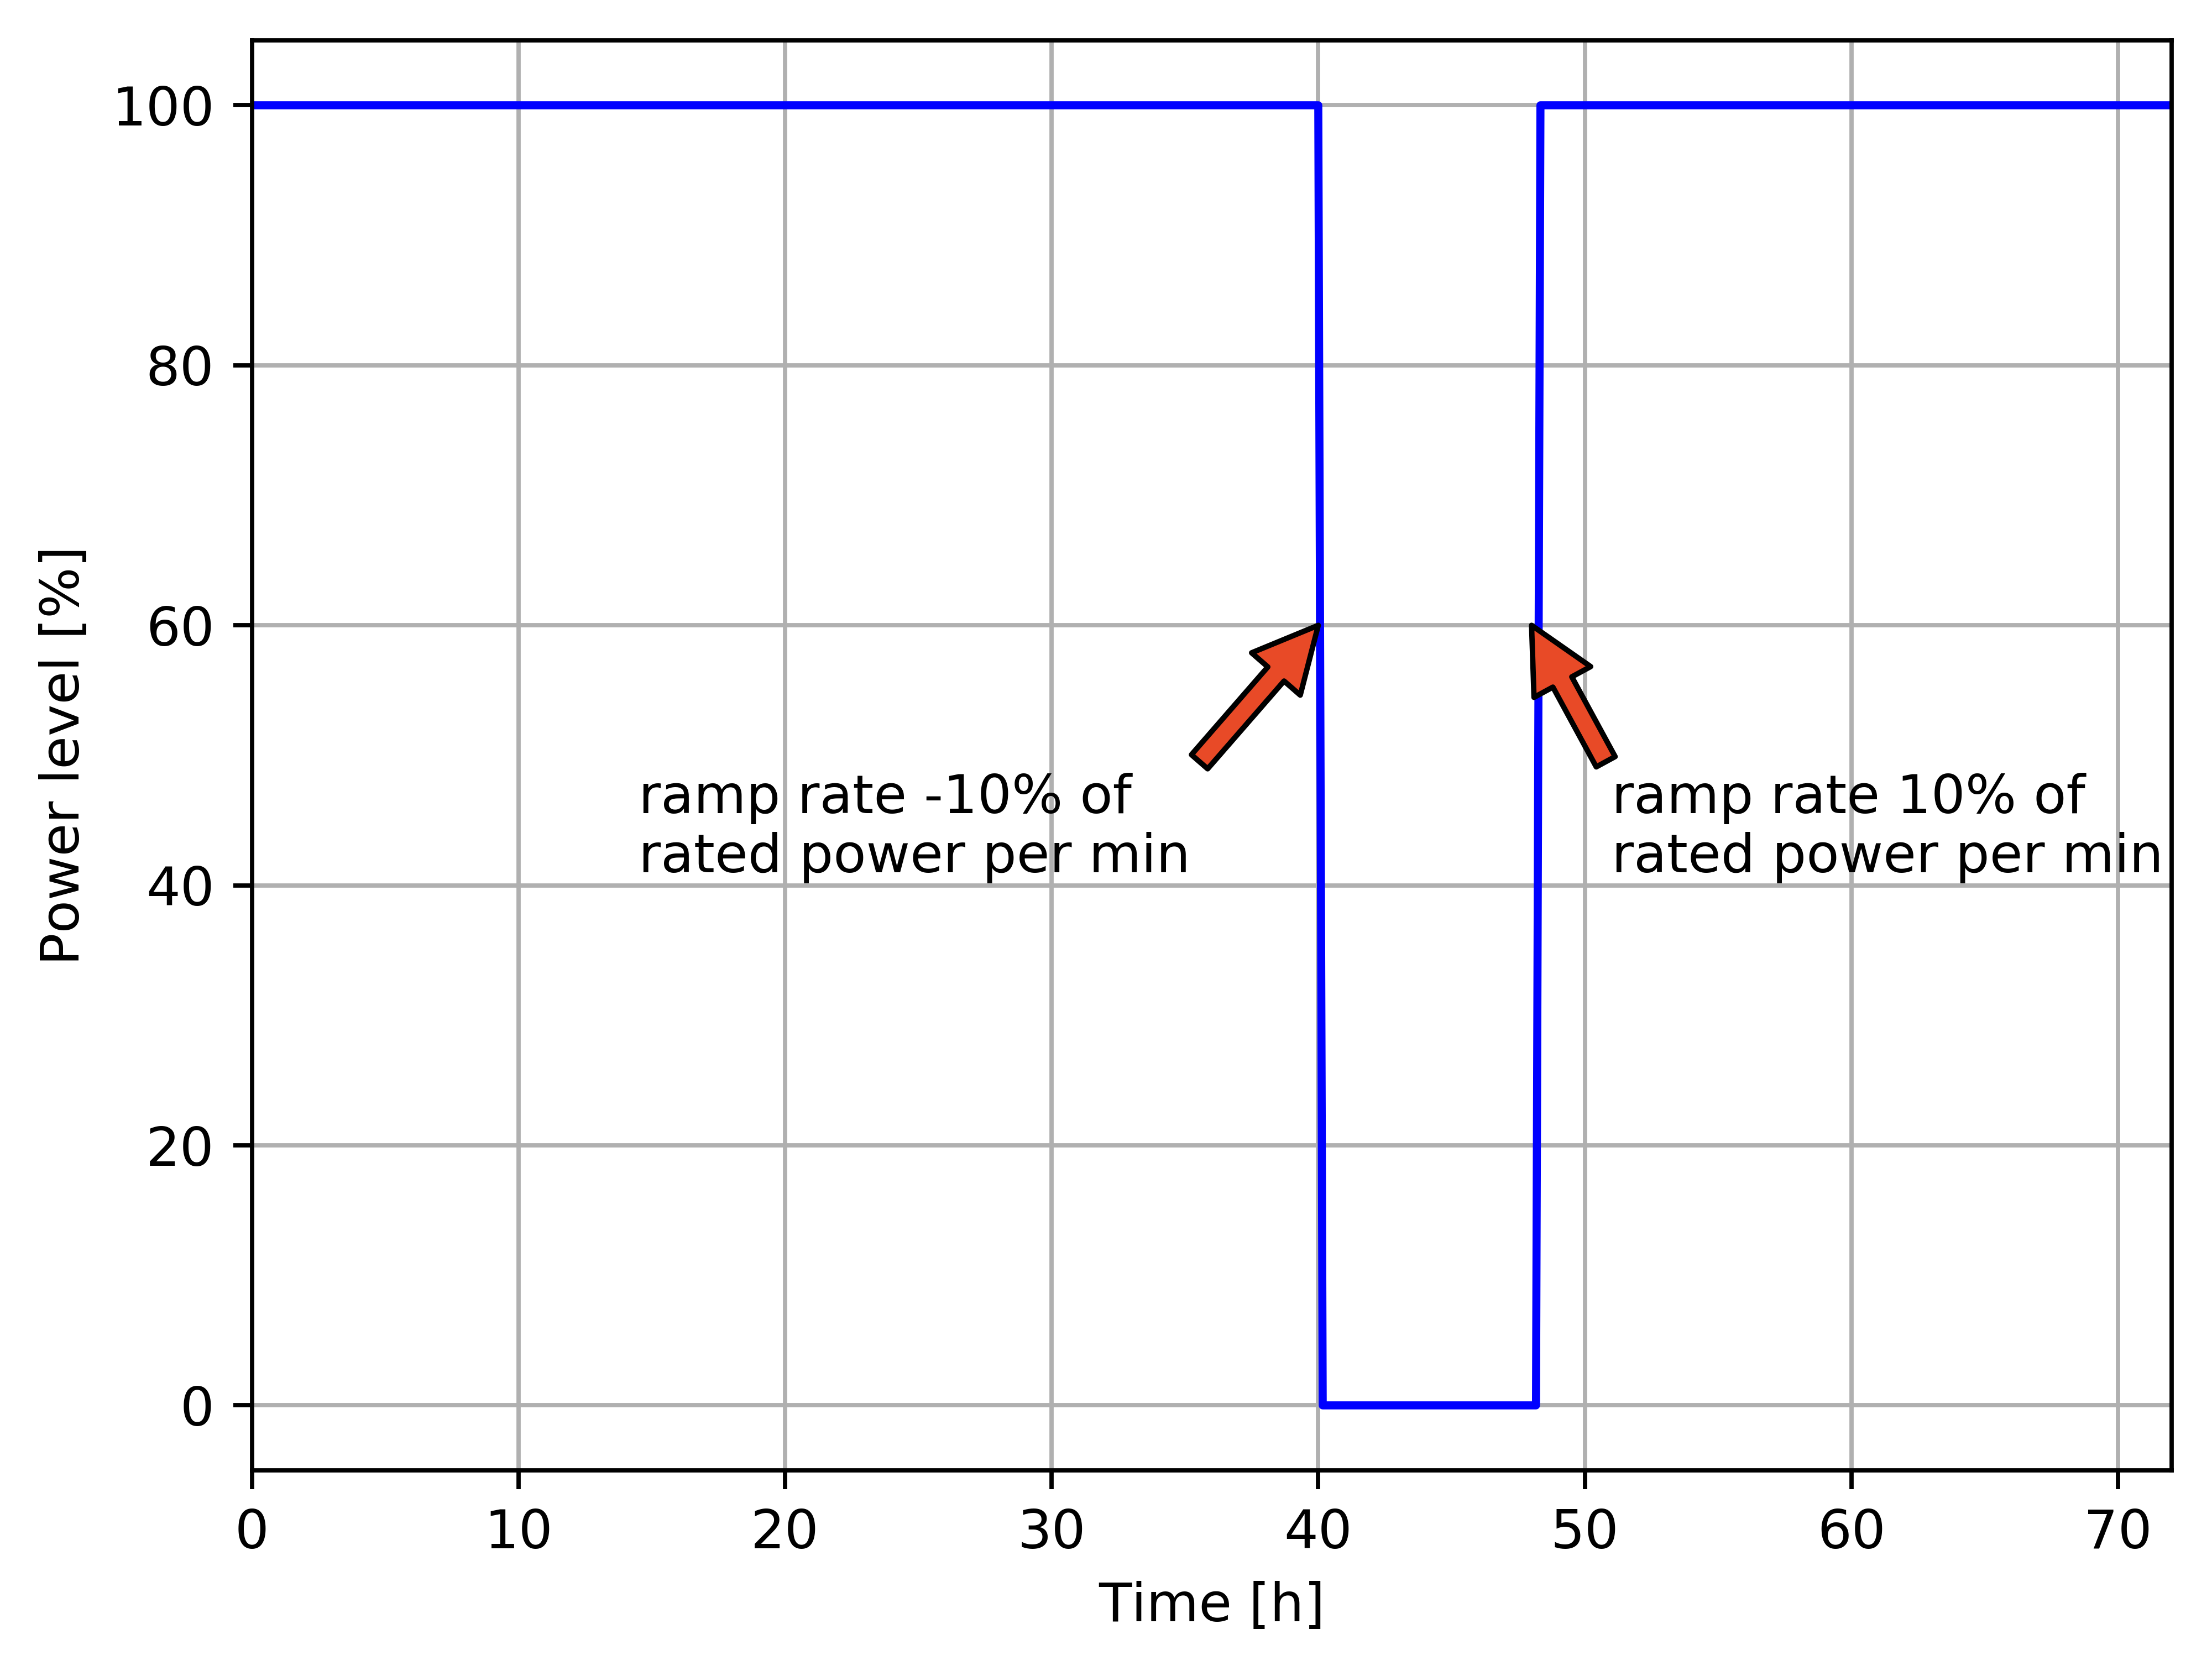
\includegraphics[width=0.8\textwidth]{load_curve.png}
	\caption{Tentative load curve for short-term load-following depletion 
	simulation for the \gls{TAP} reactor using SaltProc v1.0.}
	\label{fig:load}
\end{figure}

The depletion step time for short-term simulation will be varied in a range 
from 1 to 60 min to find a compromise between accuracy and computational cost. 
It is expected that load-following performance will be better at the \gls{BOL} 
because the neutron energy spectrum thermalizes during the reactor operation. 
Thus, the short-term load-following simulation will be repeated for the 
\gls{BOL}, the middle of life, and the \gls{EOL} to assess the \gls{TAP} 
concept performance in a load-following regime during the whole reactor 
lifetime.

Additionally, sensitivity analysis of input parameters in the xenon extraction 
correlation will be conducted to determine the range of key parameters (e.g., 
mass transfer coefficient, helium sparging rate, gas-liquid interfacial area, 
temperature) when load-following is possible for the \gls{TAP} reactor in a 
worst-case power demand scenario. These multiple system configurations  
incorporating user-parametrized components in the fuel salt processing system 
will be collected and published in a \textit{.json}-compatible database for 
use with the SaltProc v1.0 to encourage further research in this area.

\section{Stage 4: Prototype design for the Xe removal system}
As the model becomes capable of incorporating user-parametrized components 
with correlation-based extraction efficiency for the helium sparging 
component, constraints bounding a suitable sparger design will be determined 
and described. These design ranges (i.e., helium sparging rate) obtained from 
the previous Stage. The ultimate objective of the design is to ensure 
load-following operation during most of the operation period when 
minimizing the fuel salt inventory. That is, constrained optimization problem 
must be solved to minimize total fuel salt volume outside of the core. The 
target design parameters for the sparger include: the volume of sparger, 
helium flow rate, salt flow rate, and geometry.

Additionally, nuclear criticality safety analysis will be performed using 
MCNP6 \cite{werner_mcnp6._2018} to confirm that the selected sparger design 
has a subcritical configuration. If the sparger geometry obtained during the 
optimization process is supercritical, the fission gas removal system would 
contain multiple spargers of smaller size connected in parallel. Total fuel 
salt volume and sparger size are expected to be smaller at the \gls{BOL} and 
increase steadily as the neutron energy spectrum becomes softer.

\section{Stage 5: \gls{TAP} Safety Analysis}
The objective of this Stage is to characterize neutronics limits related to 
load following. High-fidelity simulations will achieve this goal with the 
Serpent 2 Monte Carlo code. Specifically, changes in safety parameters 
(Section~\ref{sec:safety-param}) will be evaluated for two time frames:
\begin{enumerate}
	\item Long-time-scale changes in safety parameters should not compromise 
	\gls{TAP} \gls{MSR} safety.
	\item Load-following operation at key moments in the reactor lifetime 
	(e.g., at startup, at the middle of life, at the end of life) must not 
	result in significant changes in safety parameters.
\end{enumerate}
Section~\ref{sec:safety-param-res} showed preliminary calculations of  
temperature coefficients and reactivity control system worth for the \gls{TAP} 
at startup. The next step will develop a axially discretized core geometry in 
Serpent with non-uniform axial density distribution to estimate the axial 
power offset. Afterward, safety parameters will be calculated at the 
\gls{BOL}, the middle of life, and the \gls{EOL} to capture safety parameter  
variation over long time scales. Validation against previous work in a 
collaboration between Transatomic Power and ORNL 
\cite{betzler_assessment_2017, betzler_fuel_2018} will also be 
performed for confidence building. Additionally, analysis for different xenon 
removal efficiencies (i.e., in the range from 0 to 100\%) will be performed to 
capture the effect of $^{135}$Xe concentration on safety.

To analyze the impact of the load-following operation on \gls{TAP} concept 
safety, safety parameter calculations will be repeated for the load-following 
transient. The combination of fuel and moderator temperature coefficients must 
remain strongly negative, and the reactivity worth of control rods must be 
sufficient to shut down the reactor for all times during load-following 
operation. 

\section{Conclusions}
Details of gas removal and fuel salt processing systems in liquid-fueled 
\glspl{MSR} have historically been conceptual rather than concrete. Usually, 
researchers assume ideal rather than realistically constrained poison 
extraction efficiency for reactor performance calculations. This work will 
more realistically model an online molten salt processing system with a focus 
on the gas removal system of the prospective \gls{TAP} \gls{MSR}. SaltProc, a 
Python toolkit was developed as a part of this work. SaltProc couple directly 
with the Serpent 2 Monte Carlo burnup software to capture the evolution of 
fuel salt composition during reactor operation in the context of an online 
fuel processing system.

Modeling and simulation of the online reprocessing system in the \gls{MSR} 
has shown promise in past research. Our work on simulating online fuel  
reprocessing for the thorium-fueled \gls{MSBR} yielded interesting results: 
notable neutron energy spectrum shift and corresponding changes in safety 
parameters during operation. Additional preliminary work also showed promise 
results in modeling a simplified fuel processing system for the \gls{TAP} 
\gls{MSR}. These simulations motivate future work in modeling advanced 
liquid-fueled \gls{MSR} plant designs.

To establish a feasible system design for molten salt fuel reprocessing, a 
more advanced model of the \gls{TAP} \gls{MSR} system with adjustable core 
geometry and realistically achievable extraction efficiencies will be 
developed. Extended SaltProc v1.0 will realistically capture the dynamics of 
fuels salt composition changes with higher accuracy. SaltProc v1.0 will also 
be employed to simulate the \gls{TAP} \gls{MSR} behavior in short-term 
transients to determine the feasibility of load following. Additionally, input 
parameters such as flow rates, bubble size, and the void fraction will be 
varied to determine the range of these parameters when the load following is 
possible for the \gls{TAP} concept.

In addition to these simulations, several extensions are suggested to 
advance our preliminary work. First, the feasible design parameters of the 
sparger, critical component of the \gls{TAP} gas removal system, will be 
optimized through sensitivity analysis of geometry and system conditions. To 
guarantee criticality safety,an MCNP6 simulation will be performed to define 
an appropriate sparger geometry. Further effort will focus on safety  
parameter evolution in the \gls{TAP} reactor during lifetime (60 years),  
when the moderator rod configuration discretely changes. Finally, dynamics of 
the safety parameters will be investigated for a short-term case: load 
following for three days with fixed moderator configuration and worst-case 
scenario of the power level change. 



%%%%%%%%%%%%%%%%%%%%%%%%%%%%%%%%%%%%%%%%%%%%%%%%%%%%%%%%%%%%%%%%%%%%%%%%%%%%%%%
% APPENDIX
%
%\appendix
%\include{apx}

\backmatter

%%%%%%%%%%%%%%%%%%%%%%%%%%%%%%%%%%%%%%%%%%%%%%%%%%%%%%%%%%%%%%%%%%%%%%%%%%%%%%%
% BIBLIOGRAPHY
%
%\bibliographystyle{IEEE_ECE}
\bibliographystyle{unsrt}
% Put references in BibTeX format in thesisrefs.bib.
\bibliography{thesisrefs}

\end{document}
\endinput
